\documentclass[11pt]{article}
\usepackage[italian]{babel}
\usepackage[utf8]{inputenc}
\usepackage{graphicx}
\usepackage{float}
\usepackage{amsmath}
\usepackage{amsfonts}
\usepackage{hyperref}
\usepackage{glossaries}
\makeglossaries
\newglossaryentry{domain}{
    name=domain,
    description={Si intendono, qui, le conoscenze relative ad un determinato ambito. Ad esempio, sviluppando un sistema per Trenitalia(\textit{qualcuno lo fa veramente? Non sono scritti da scimmiette?}), il dominio sarebbe quello della gestione dei treni. Il problema sta nel fatto che il programmatore non ha conoscenze al riguardo dei treni, e deve utilizzare quindi un linguaggio, implicazioni e conoscenze che non gli appartengono}
}
\newglossaryentry{volatility}{
    name=volatility,
    description={Con RV intendiamo modifiche ai requirements che avvengono durante lo sviluppo del progetto. \textit{(Il classico "Ah ma già che ci sei, mi aggiungi un ecommerce, una macchina del caffè, e la possibilità di accarezzare i clienti attraverso il computer? Maledetti)}}
}
\newglossaryentry{case}{
    name={CASE tool},
    description={Il CASE tool è un software che supporta la progettazione di sistemi software, ad esempio con UML}
}
\newglossaryentry{constraint}{
    name={constraint},
    description={un constraint è un limite che viene posto; restriction, limitation.}
}
\usepackage[normalem]{ulem}
\newcommand{\code}[1]{\texttt{#1}}
\newcommand{\numpy}{{\tt numpy}}    % tt font for numpy
\topmargin -.5in
\textheight 9in
\oddsidemargin -.25in
\evensidemargin -.25in
\textwidth 7in
\begin{document}

% ========== Edit your name here
\author{Simone Montali\\monta.li}
\title{Riassunti di Ingegneria del Software}

\maketitle

\medskip
\section*{Prefazione}
Questo progetto nasce dalla necessità di trovare un metodo di studio per questa materia che, ai più sembra banale. Il problema di fondo è proprio in questa apparente banalità: si finisce per studiarla di fretta pensando di conoscerla, e ci si rende conto troppo tardi di non essere pronti. Mi scuso, anzitutto, per il vocabolario misto italiano-inglese che utilizzerò in queste pagine. Tanti di voi sanno quanto sia complicato esprimere certi concetti in italiano. Ho inserito un piccolo glossario a fine documento. Questo documento ha lo scopo di essere il giusto mezzo tra completezza e sinteticità. Mi scuso, in secundis, per i toni a volte scurrili. Un vero informatico è arrabbiato \textit{/per il codice che non compila/\LaTeX  che fa ciò che vuole/il computer che si impalla/quel piccolo bugfix di Linux che diventa un bagno di sangue/}, e non c'è modo migliore di sfogare le incazzature informatiche che imprecare in riassunti che leggeranno le generazioni a venire. 
Non so come tu ti sia procurato questo documento, ma se hai 5 minuti da buttare, dai una letta alle cose che ho scritto \href{https://monta.li/appunti}{qui.} Ci troverai anche un'altra valangata di appunti. Buona studiata ed in bocca al lupo per tutto.
\section{T1 - Software Development Process}
Anche la signora seduta all'angolo di via Cavour, sa che oggi più che mai i software sono parte di tutti i processi che fanno girare il mondo. L'Ingegneria del software è però molto di più che scrivere codice. Infatti, è piuttosto un concetto di risoluzione dei problemi del mondo reale, sfruttando software. I requirements sono sempre più stringenti: tempi brevi, sistemi complessi, molte funzionalità richieste. Un buon software deve avere ottime \textbf{maintainability, dependability, efficiency, acceptability}. Problemi e soluzioni sono complessi, ma il software offre estrema flessibilità. Esso è un sistema discreto. Alcuni problemi tipici possono essere le scadenze, i budget, le performance, la manutenzione. Le sfide principali sono rappresentate da \textbf{eterogeneità, delivery, trust.} L'attività di problem solving è composta da due fasi: l'analisi e la sintesi. 
\subsection{Quindi? Cos'è l'ingegneria del software?}
Siamo giunti al nocciolo della questione: \textbf{di cosa stiamo parlando?} L'ingegneria del software è un insieme di \textbf{tecniche, metodologie, strumenti} che aiutano nella produzione di software di alta qualità dati un budget, una scadenza, e delle modifiche continue. La sfida principale è quindi quella di avere a che fare con complessità elevate. 
Siamo di fronte anche a un aumento delle responsabilità: un ingegnere del software non deve solo scrivere codice, ma piuttosto lavorare con competenze e confidenzialità, applicando un'etica.
\subsubsection{Processo del software}
In seguito ad una rappresentazione astratta, si procede con un set di attività strutturato: specifica dei \textbf{requirements}, \textbf{design}, \textbf{implementazione}, \textbf{validazione}, \textbf{evoluzione}. 
\subsection{Modelli di sviluppo del software}
Distinguiamo tra \textbf{plan-driven} e \textbf{agile} development. Nel primo, prima si pianificano i requirement, e solo in seguito si sviluppa il software. Nel secondo si sviluppa il software un pezzo alla volta, a stretto contatto col cliente. 
\subsubsection{Modello a cascata}
In questo modello, \textbf{plan-driven}, le specifiche e lo sviluppo sono separati. I pro sono, ad esempio, un'ottima documentazione e manutenzione semplice. D'altro canto, però, le specifiche vengono \textit{"congelate"} dopo la prima fase, il cliente viene poco coinvolto, ed i tempi sono più lunghi. 
\begin{figure}[H]
    \centering
    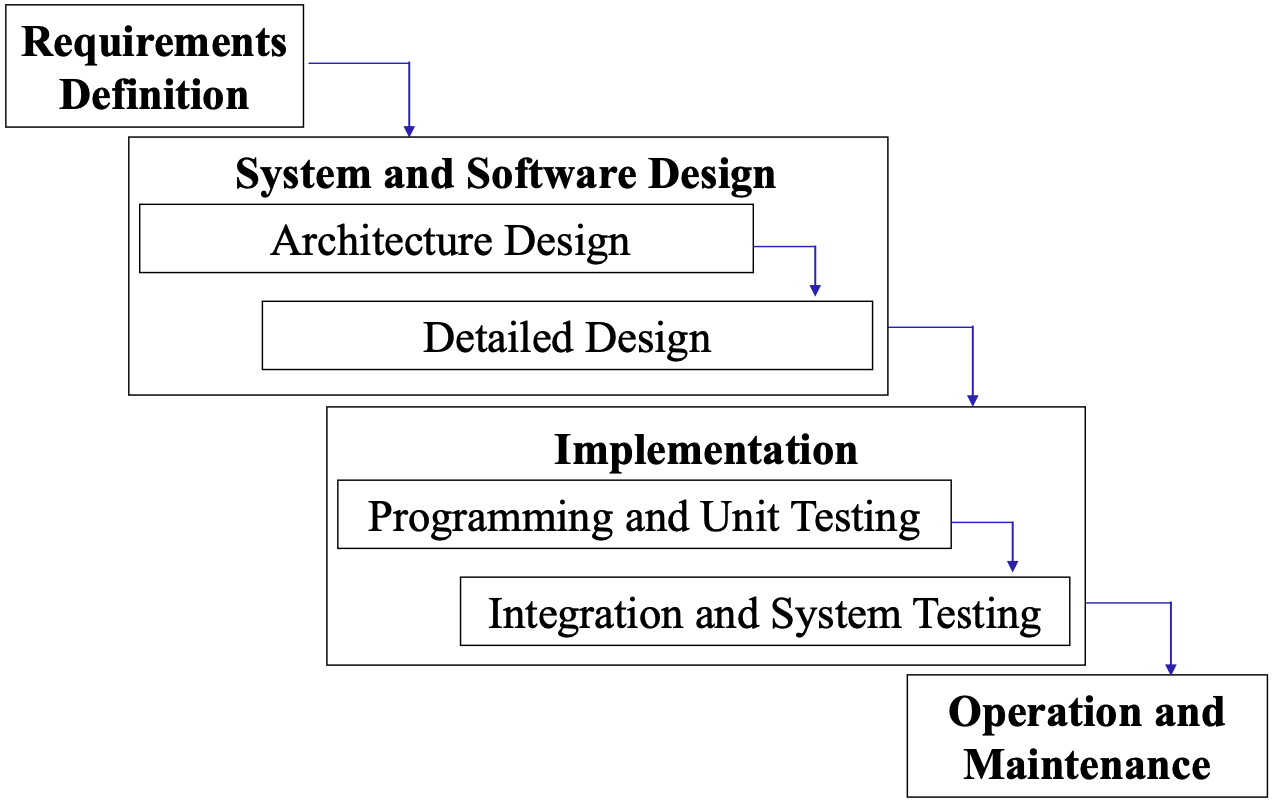
\includegraphics[width=\linewidth]{res/teoria/WaterfallModel.png}
    \caption{Waterfall Model}
\end{figure}
\subsubsection{Modello a spirale}
Nel modello a spirale, abbiamo diverse fasi che si susseguono a spirale; il \textit{risk handling} viene gestito tramite prototipazione, che permette di testare i prodotti contro i requirements. Alcuni pro possono essere l'elevata prevenzione dei rischi, la completezza della documentazione, la flessibilità. È, però, un modello costoso, riservato ad esperti ed a progetti costosi e richiedenti molta sicurezza. La spirale può allargarsi all'infinito. Il \textbf{prototipo} è un'implementazione limitata del sistema, rappresentando solo alcuni aspetti. È utilizzato in varie fasi dello sviluppo. Porta però vari vantaggi, come un'elevata usabilità, un buon design, una grande facilità di manutenzione, ed un ridotto costo di sviluppo. 
\begin{figure}[H]
    \centering
    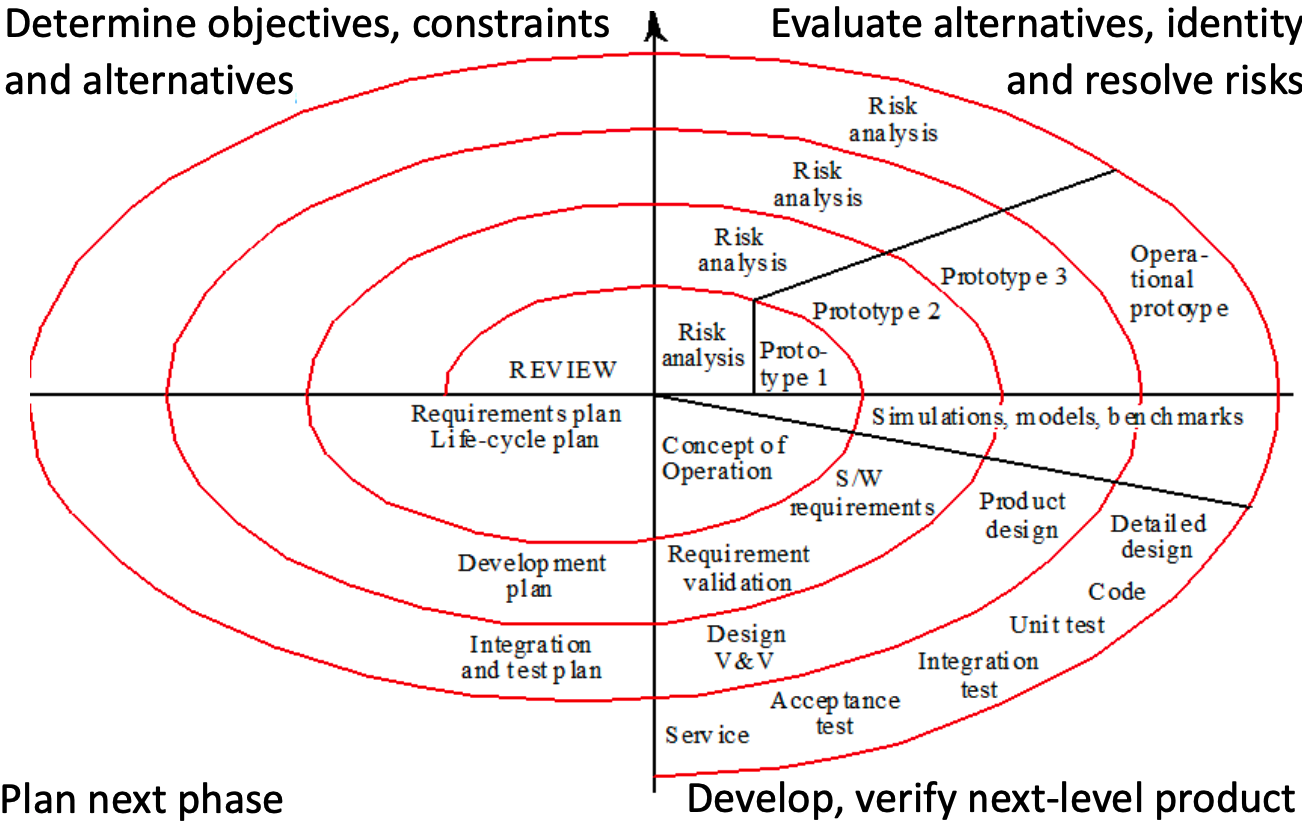
\includegraphics[width=\linewidth]{res/teoria/SpiralModel.png}
    \caption{Spiral Model}
\end{figure}
\subsubsection{Incremental development}
L'incremental development consiste in una prima fase di raccolta dei requirement, da cui nasce la versione iniziale, una fase di design, ed una fase di implementazione, che produce la versione finale. Alcuni pro possono essere la naturale presenza di prototipi ad ogni aggiunta di feature, un basso rischio di fallimento progettuale, una quantità di testing variabile in base alla priorità. Alcuni contro: bassa \textit{process visibility}, sistemi mal strutturati, skill speciali necessarie. Esso è adatto per progetti piccoli, o parti di progetti grandi. 
\begin{figure}[H]
    \centering
    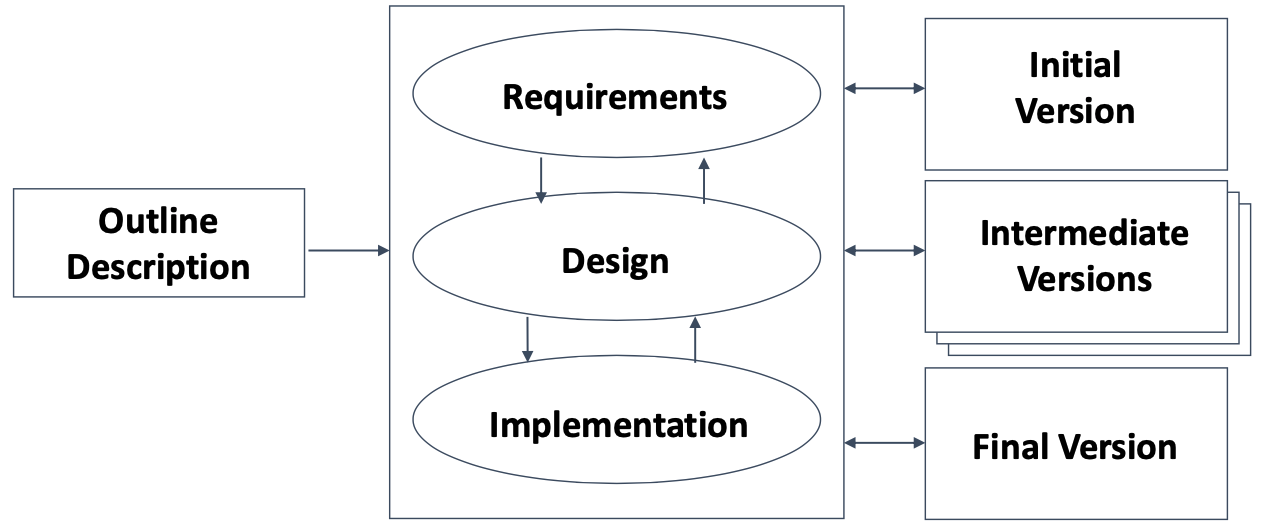
\includegraphics[width=\linewidth]{res/teoria/IncrementalDevelopment.png}
    \caption{Incremental Development}
\end{figure}
\subsubsection{Test driven development}
Qui, i test vengono scritti prima dell'implementazione, rendendo note le difficoltà da subito. Rende il debug più semplice. Si aggiunge un test, si prova il codice vecchio con il test nuovo, si aggiunge la feature e si verifica che il test sia ancora positivo. 
\subsubsection{Agile development}
\textit{"Tutti fanno Agile, nessuno fa Agile."} L'agile è basato sulla \textbf{continuous delivery}, con dei requirements in continuo cambiamento. Il cliente è direttamente coinvolto, aggiungendo requirements man mano che il progetto va avanti. È una metodologia semplice nella quale il team si auto organizza, ma ha svariati rischi, come la mancanza di planning, la necessità di team esperti, la documentazione scarna o spesso errata. 
\subsubsection{Extreme Programming}
\textit{Suona più badass di quanto sia realmente/s} L'XP è utilizzato in situazioni in cui i requirements variano velocemente, i team sono ridotti e "affiatati"(spesso si ricorre al \textbf{pair programming}). È un tipo di programmazione agile, basato su design semplice, release minori, refactoring continuo, alta semplicità. 
\begin{figure}[H]
    \centering
    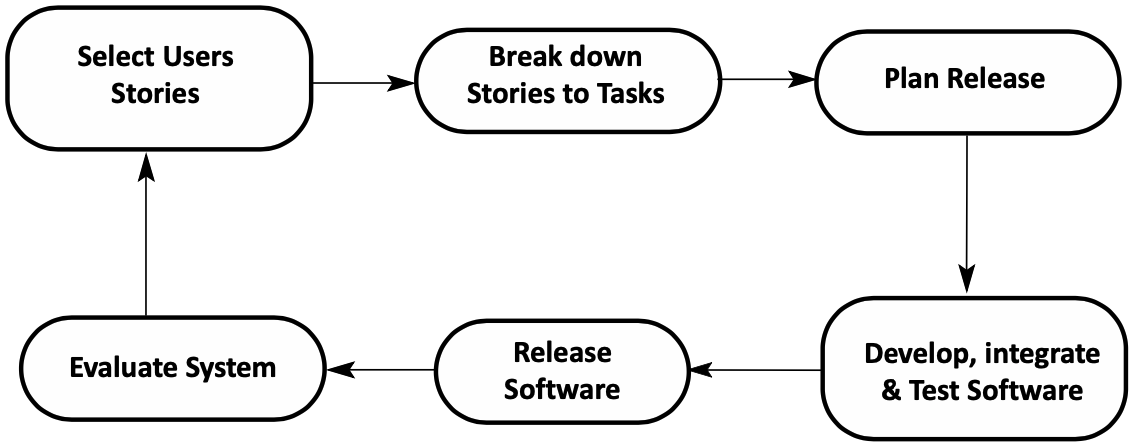
\includegraphics[width=\linewidth]{res/teoria/ExtremeProgramming.png}
    \caption{Extreme Programming}
\end{figure}
\subsection{Reusable software}
È spesso comodo lavorare per \textbf{microservizi} atomici, in modo da poterli riutilizzare. Parliamo, ad esempio, di API. Questo riduce i costi e i tempi di sviluppo, al costo di leggeri sacrifici sul lato dei requirements, e un mancato controllo sull'evoluzione del software $\rightarrow$ funzionalità che variano il loro comportamento. \textit{Parlo a lei, signor React (ah, già, Mark), che cambia tutto ad ogni versione.} 

\section{T2 - Coding, Debugging, Testing} 
Un buono stile di coding è fondamentale perché i programmi vengono scritti una volta, ma letti molte. Alcuni aspetti importanti sono il layout, i nomi, i commenti. 
\subsection{Legge di Ambler per gli standard}
Più uno standard è utilizzato, più è facile comunicare tra membri del team. Si possono inventare standard quando necessario, ma attenzione a non perdere tempo in qualcosa che non verrà riutilizzato. 
Tutti i linguaggi hanno standard reperibili. \textit{Consiglio per la vita: quando vi servono, esistono \href{https://google.github.io/styleguide/}{gli standard di Google}, gente più affidabile di me.} È consigliabile avere standard aziendali. Uno standard consiste di nomenclature, formattazione, formato e contenuto dei commenti. È necessario documentare tutte le volte in cui si infrangono gli standard. \textit{(È davvero necessario infrangerlo?)}
\subsection{Coding practices}
Alcune pratiche sono rappresentate da:
\begin{itemize}
    \item \textbf{indentazione}, che oltre ad essere importante per la leggibilità, a volte fa parte delle regole di compilazione. \textit{e.g. Python.}
    \item \textbf{whitespaces}, migliorano la leggibilità. \textit{Però, non fate le bestie di satana mettendo uno spazio dopo l'apertura della parentesi. Non fatelo. }
    \item \textbf{Naming, commenting}, rendono la comprensione del codice molto più facile.
\end{itemize}
I commenti sono uno strumento fondamentale da tenere sempre vicino al codice. Non pensiate però di essere autorizzati a scrivere \textit{spaghetti code}, se commentato. Refactorate. Fondamentale è spiegare i compiti di classi, funzioni, variabili o blocchi di codice complessi. \textit{In generale, se avreste bisogno di spiegarlo a Guido Soncini, commentatelo}. Utilizzare uno standard permette ai vostri colleghi di non dover riscrivere il vostro codice perché non gli piace. Rendete più semplice aggiungere funzioni, o creare la documentazione. È, insomma, tempo ben speso. 
\subsection{Dealing with errors}
Distinguiamo tra prima, durante e dopo: \textbf{prevention, detection, recovery}. Alcune fonti di errori possono essere un design errato, una mancanza di isolazione, o typos. Per esempio, errori di "confini" negli array, errori di \textit{off-by-one}, errori di input errati. Per debuggare, bisogna riconoscere l'esistenza di un bug, isolarne la fonte, identificarne la causa, trovare un fix, applicarlo, e \textbf{testarlo}. \textit{Lo scrivo in grassetto perché mi capita spesso di rompere più di quello che metto a posto.} 
Riconoscere un bug spesso è complicato, soprattutto quando accade solo in determinate situazioni, o se il software è difficile da testare. Per trovare i bug, potete usare dei print statement, molto veloci da usare ma spesso incompleti e poco pratici. Per questo, esistono gli strumenti di debug, che permettono di bloccare il codice in determinati punti, analizzare le variabili, \textit{e bestemmiare con calma.} Spesso gli errori sono dovuti al design piuttosto che all'implementazione. 
\subsection{Testing}
Il testing permette di scovare errori e bug, ma non la loro assenza. È purtroppo impossibile testare ogni caso. Il tester deve conoscere il sistema e le tecniche di testing. \textbf{Il tester non dovrebbe essere il programmatore.} Spesso il programmatore ha in mente il modo corretto di far funzionare il programma, e quindi difficilmente trova casi in cui il suddetto si rompe. 
\subsubsection{Unit testing}
Lo unit testing permette di testare singole unità di codice, trovando falle negli algoritmi, i dati, la sintassi. Un set di test cases viene creato e poi utilizzato. 
\subsubsection{Integration testing}
L'integration testing prova un gruppo di sottosistemi, o anche l'intero software. Viene eseguito dai programmatori, il goal è testare le interfacce oltre ai sottosistemi. 
L'intero sistema è visto come un insieme di sottosistemi, l'obiettivo è quello di testare tutte le interfacce e l'interazione tra sottosistemi. La strategia determina il modo in cui i sottosistemi vengono testati. Molte falle sono date da problemi nell'interazione tra sottosistemi. Le falle non intercettate in questa fase diventeranno molto più costose. 
\subsubsection{System Testing}
Il system testing testa l'intero sistema, per verificare che rispetti i requirements funzionali e non, oltre alle prestazioni. 
\subsubsection{Functional Testing}
Questo tipo di testing viene svolto per verificare la funzionalità del sistema. I test cases vengono ideati a partire dai requirement del progetto, ed il sistema è trattato come una black box. 
\subsubsection{Performance Testing}
Questo tipo di testing tenta di provare il sistema in situazioni estreme, come alti carichi, input errati, grandi volumi di dati. Alcuni esempi sono stress testing, security testing, volume testing, recovery testing.
\subsubsection{Acceptance Testing}
Questo tipo di testing prova che il sistema sia effettivamente pronto per la fase di production. I test vengono scelti ed effettuati dal cliente. Questi sono i famosi \textbf{alpha e beta tests.} Nel primo, il software è ancora nell'environment di sviluppo. Nella beta, l'environment è quello del cliente e l'utilizzo effettuato è realistico. 
\section{T3 - System Modeling and UML}
Il system modeling fornisce rappresentazioni astratte a problemi reali, tramite notazione grafica. Un modello funzionale dovrebbe introdurre i componenti essenziali, utilizzare una notazione \textit{consistente}, ed utilizzare tool al supporto della creazione. Il modello esprime quindi la realtà, adattata a dei modelli standard. Il system modeling deve essere \textbf{predictive}, in quanto deve essere svolto prima del development. Dev'essere \textbf{extracted} da un sistema esistente, tramite analisi delle proprietà del software. Deve essere \textbf{prescriptive}, ossia definire un set di regole e limiti per l'evoluzione del software. 
\subsection{UML}
Unified Modeling Language nasce per unire diversi standard/linguaggi di modellazione, con diagrammi multipli e interoperabilità. UML è \textbf{semplice, espressivo, utile, consistent, estensibile}. Alcuni esempi di views sono:
\begin{itemize}
    \item Use Case view
    \item Structural view
    \item Behavioral view
    \item Implementation view
    \item Environment view
\end{itemize}
\begin{figure}[H]
    \centering
    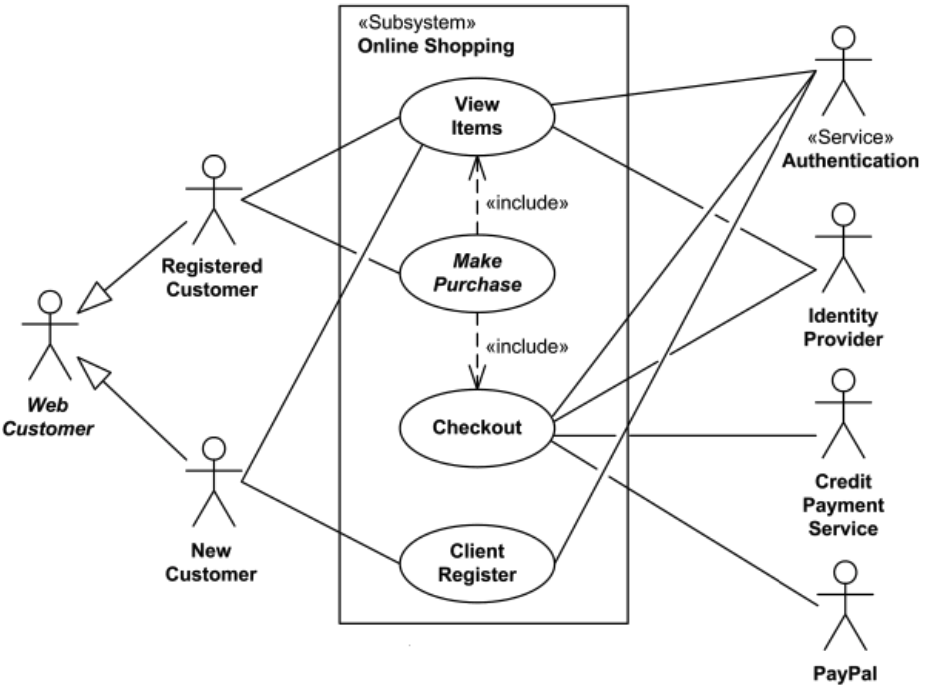
\includegraphics[width=0.6\linewidth]{res/teoria/UseCase.png}
    \caption{Use case diagram}
\end{figure}
\begin{figure}[H]
    \centering
    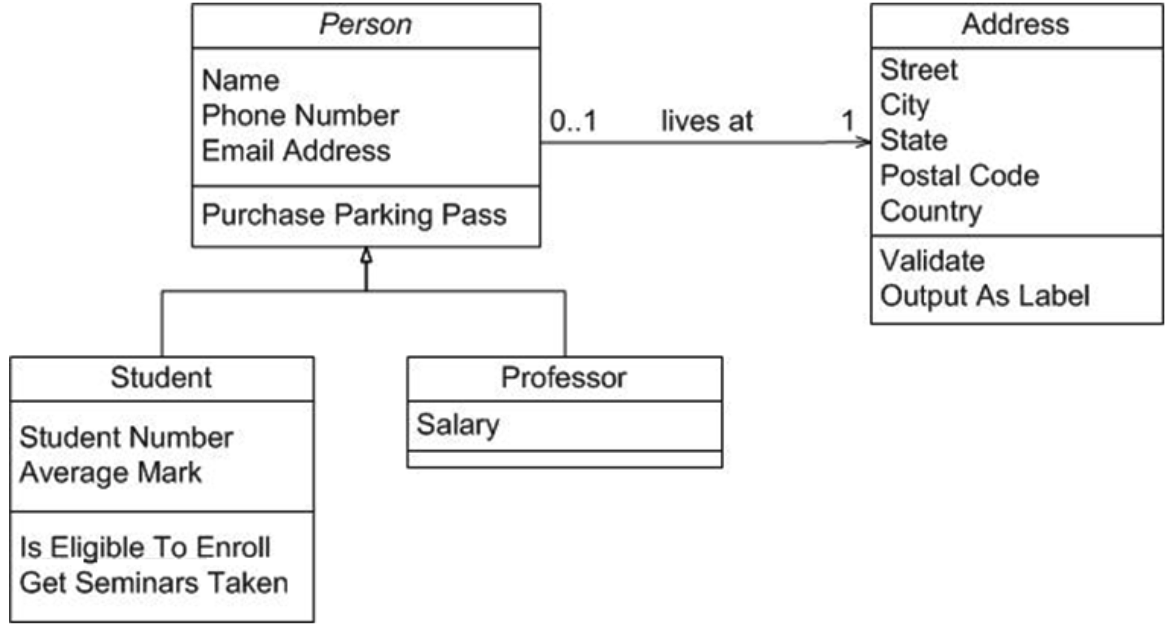
\includegraphics[width=0.6\linewidth]{res/teoria/ClassDiagram.png}
    \caption{Class diagram}
\end{figure}
\section{T4 - Requirements Engineering}
Gli scopi del requirements engineering sono \textbf{identificare} i servizi necessari ed i constraint, \textbf{definire} offerta e contratto, \textbf{ottenere} tutte le informazioni necessarie al design. I desiderata sono:
\begin{itemize}
    \item \textbf{Validi}, esprimendo le reali necessità
    \item \textbf{Non ambigui}, leggibili in un solo modo 
    \item \textbf{Completi}
    \item \textbf{Comprensibili} da tutte le persone coinvolte 
    \item \textbf{Consistent}, non possono contraddirsi 
    \item \textbf{Prioritizzati}, a volte bisogna scegliere
    \item \textbf{Verificabili}, con test 
    \item \textbf{Modificabili} senza difficoltà
    \item \textbf{Traceable}, la loro origine è chiara
\end{itemize}
\subsection{Some requirements classifications}
\subsubsection{Functional requirements (System Feature)}
Descrivono funzionalità di sistema o di servizi, come l'input di dati, operazioni svolte, workflow, dati in output, autorizzazioni. Ad esempio, in una biblioteca, un functional requirement può essere la ricerca di libri da parte di un socio.
\subsubsection{Non-functional requirements (System Feature)}
Descrivono \glspl{constraint} di parti del sistema e del suo sviluppo. Specificano criteri per giudicare l'operato del sistema. Con l'esempio di prima, i libri devono avere un codice che rispetti lo standard ISBN, e il sistema non deve rilasciare informazioni sensibili sui soci a determinati autorizzati. 
Alcune metriche per questi requirements possono essere velocità, dimensione, facilità d'uso, affidabilità, robustezza, portabilità.
\subsubsection{Domain requirements (System Feature)}
I \gls{domain} requirements derivano dal dominio dell'applicazione, ossia l'ambito in cui si lavora. 
\subsubsection{Volatile Requirements (Static/Dynamic Nature)}
I \textbf{mutable requirements} sono requirements destinati a cambiare, come normative o tasse. Gli \textbf{emergent requirements} cambiano quando il cliente capisce di più sul sistema. I \textbf{consequential requirements} emergono con l'informatizzazione di un sistema che non lo era. I \textbf{compatibility requirements} emergono dal doversi interfacciare con altri sistemi appartenenti all'organizzazione. 
\subsection{Rischi}
Alcuni rischi nella scrittura dei requirements possono essere:
\begin{itemize}
    \item Imprecisioni
    \item Conflitti tra più requirements
\end{itemize}
\subsection{Documento di specifica dei requirements}
Il \textbf{documento di specifica dei requirements} specifica i requirement di sistema, includendone una definizione e una specifica. È detto \textbf{System Specification} se include direttive su hardware e software, \textbf{Software Requirements Specification} (SRS) se include il solo software. Dovrebbe seguire lo standard IEEE 830. Un SRS deve avere un'\textbf{introduzione}, una \textbf{descrizione generale} ed infine \textbf{le feature e i requirement.} Dovrebbe avere un formato stratificato, notazioni grafiche e termini consistenti, acronimi chiari, indice, glossario, ed uno stile non ambiguo. A tal proposito, il linguaggio naturale spesso nasconde delle insidie: mancanza di chiarezza, ambiguità, troppa flessibilità... Bisogna quindi inventare uno standard di utilizzo del linguaggio naturale, con sintassi fissa, termini chiari. Alcune keyword sono: \textbf{shall, should, can, must, may, will, might, expected to, could.} Alcune alternative al linguaggio naturale possono essere un linguaggio naturale strutturato, linguaggi di descrizione del design, notazioni grafiche, notazioni formali. I rischi del processo di specifica sono una mancanza di comprensione, requirements che cambiano rapidamente, imprecisione nella stesura del documento, difficoltà nel conciliare conflitti. 

\section{T5 - Requirement engineering and UML}
\subsection{Use case diagram}
Nello use case diagram includiamo tutti i casi d'uso del sistema, da parte di diversi \textbf{attori}, rappresentanti utenti, ma anche servizi o sistemi. Il \textbf{system boundary} divide l'esterno e l'interno del sistema, gli use case dagli attori. Un attore può generalizzare un altro attore. Idem per gli use case. Uno use case può contenere la funzionalità di un altro use case. Uno use case può essere usato per estendere il comportamento di un altro use case, anche con condizioni. Opzionalmente, possiamo includere le molteplicità delle relazioni. 
\subsection{Class diagram}
Una classe è rappresentata da un rettangolo che mostra il nome della classe, e opzionalmente il nome degli attributi e delle operazioni. Il nome della classe, gli attributi e le operazioni sono separati in compartimenti. Il simbolo che precede attributi e operazioni ne indica la visibilità: $+$ se pubblico, $-$ se privato, $\#$ se protetto, \textasciitilde se package. Un'\textbf{interfaccia} è una specifica di comportamento che deve essere implementato o, più semplicemente, un \textbf{contract.} Un \textbf{template} definisce un pattern i cui parametri rappresentano tipi, e può essere applicato a classi, packages, operazioni. 
\subsubsection{Associazione}
Un'associazione è una relazione tra elementi, che implica che uno dei due sia una variabile dell'altro. Essa è rappresentata da un connettore che può includere ruoli, cardinalità, direzione e \glspl{constraint}. Per più elementi, si può usare un \textbf{diamond}. 
\begin{figure}[H]
    \centering
    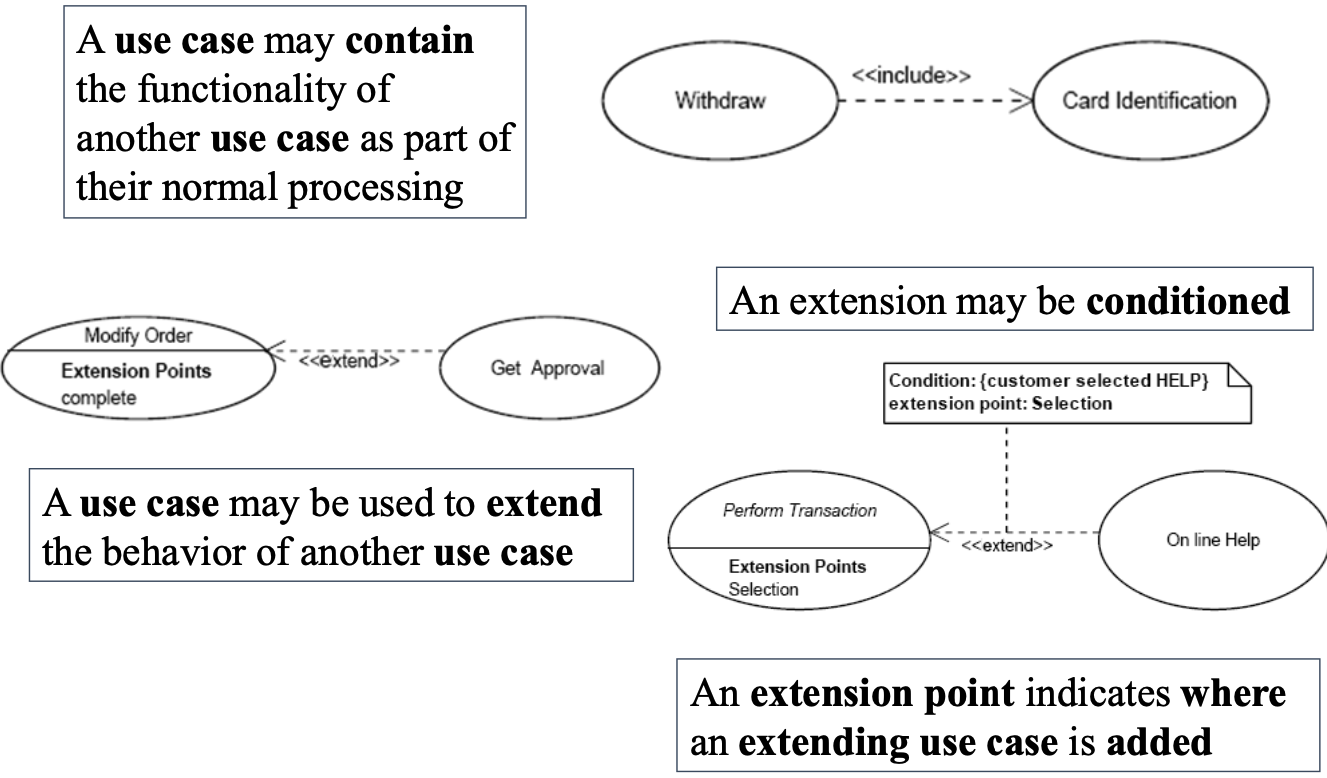
\includegraphics[width=0.6\linewidth]{res/teoria/Extension.png}
    \caption{Extension}
\end{figure}
\subsubsection{Generalization e nesting}
La generalizzazione indica \textbf{ereditarietà}, disegnata come una freccia che parte dal figlio e arriva al padre. Il connettore di nesting indica che una classe è nested nella classe dove arriva l'operatore. Con ciò, intendiamo che essa è definita all'interno del target. 
\begin{figure}[H]
    \centering
    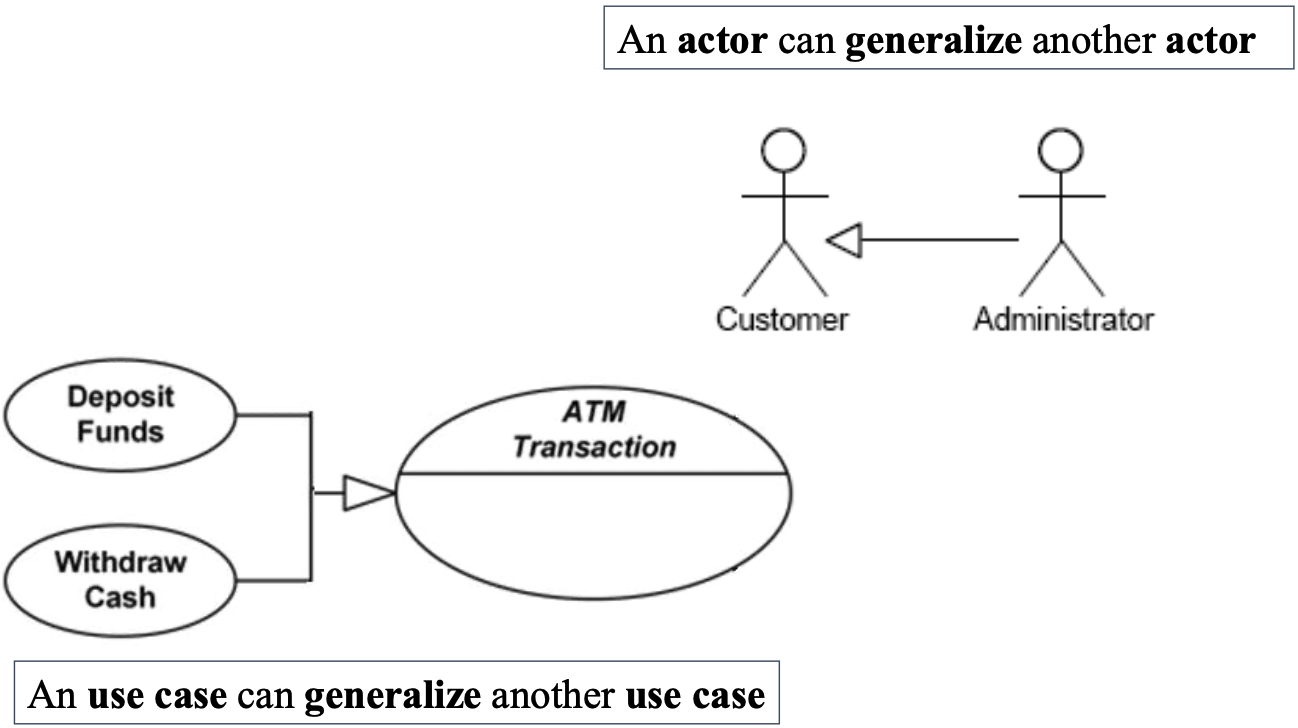
\includegraphics[width=0.6\linewidth]{res/teoria/Generalization.png}
    \caption{Generalization}
\end{figure}
\subsubsection{Dipendenza e realizzazione}
La \textbf{dipendenza} è una forma debole di relazione, e mostra un'interazione tra un client ed un supplier. La \textbf{realizzazione} è una relazione tra una specifica e la sua implementazione. 
\subsubsection{Aggregazione e composizione}
L'aggregazione rappresenta elementi composti da elementi minori. È indicata da un diamante bianco che punta verso il contenitore. I componenti possono essere condivisi da più contenitori. La composizione è rappresentata da un diamante nero. Una classe di associazione rappresenta invece un'associazione più complessa, che ha operazioni e attributi.
\begin{figure}[H]
    \centering
    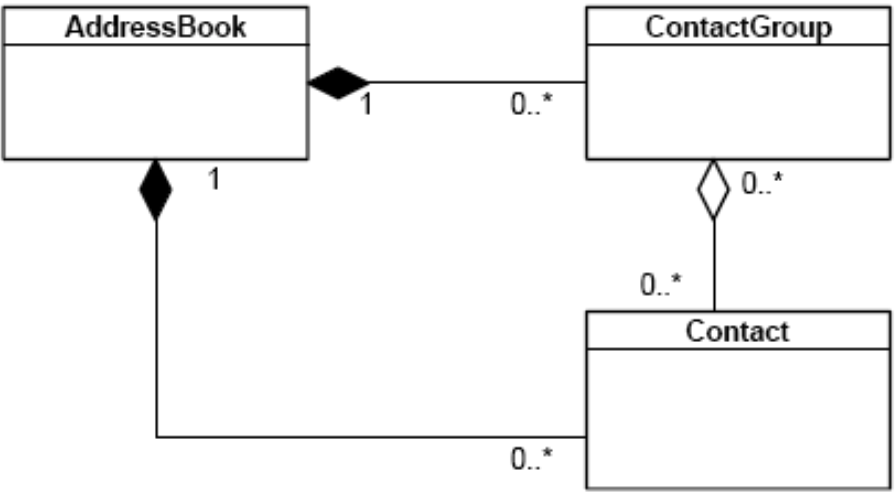
\includegraphics[width=0.6\linewidth]{res/teoria/AggrComposition.png}
    \caption{Aggregazione e composizione}
\end{figure}
\subsection{Sequence diagram} 
Il sequence diagram indica, su una \textit{lifeline (aka timeline)} verticale, l'interazione tra le classi. Se il nome della lifeline è \textit{self}, la suddetta rappresenta il classifier a cui appartiene il diagramma. Una \textbf{lifeline} rappresenta un \textit{partecipante} del sequence diagram. Possiamo avere diversi tipi di messaggi tra lifeline: sincroni, asincroni, risposte, persi, trovati, self (ricorsività). Per rappresentare logica procedurale come if, cicli, thread, usiamo i \textbf{fragment}. 
\begin{figure}[H]
    \centering
    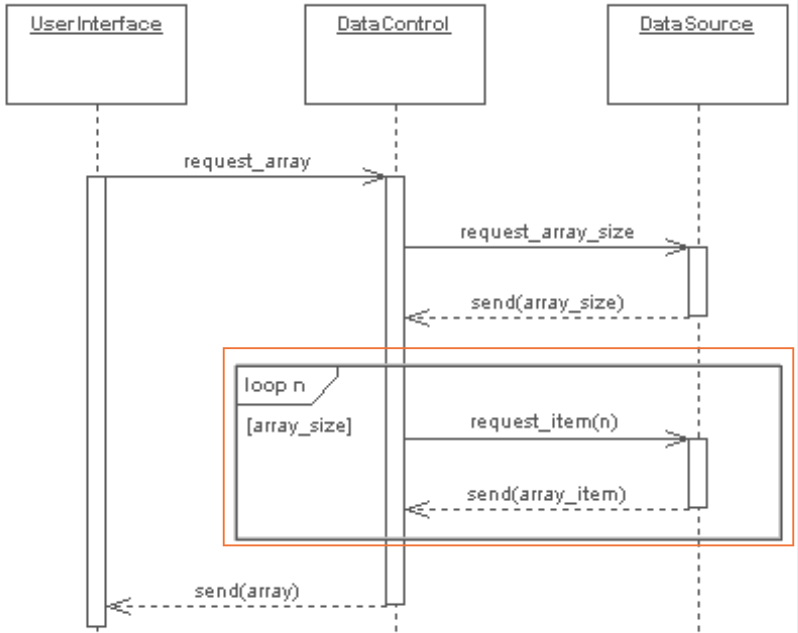
\includegraphics[width=0.6\linewidth]{res/teoria/SequenceDiagram.png}
    \caption{Sequence Diagram con fragment}
\end{figure}
\subsection{Activity diagram}
Un \textbf{activity diagram} è un diagramma di flusso che rappresenta un'operazione eseguita sul sistema, con decisioni, I/O, fork/join, timeout/segnali, concorrenza. Possiamo raggruppare alcune attività \textit{related}. 
Alcuni esempi di activity diagrams strani:
\begin{itemize}
    \item \textbf{State machine diagram}, che dà indicazioni a livello hardware
    \item \textbf{Choice and Junction pseudo state}
    \item \textbf{Compound state} tramite il quale possiamo separare alcune parti del diagramma e "includerle"
    \item \textbf{History state and concurrent regions}, con il primo indichiamo un salvataggio dello stato, col secondo due frazioni di diagramma che si svolgono contemporaneamente
\end{itemize}
\begin{figure}[H]
    \centering
    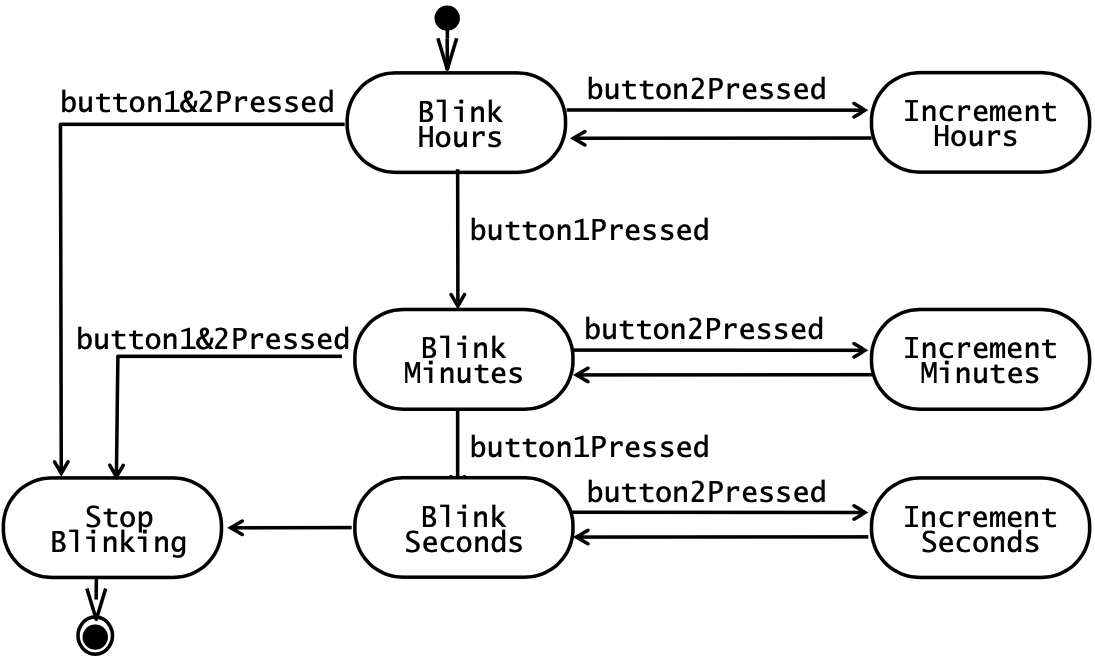
\includegraphics[width=0.6\linewidth]{res/teoria/StateMachine.png}
    \caption{State machine diagram}
\end{figure}
\subsection{Robustness diagram}
Il \textbf{robustness diagram} è un UML semplificato che ha lo scopo di raffinare gli use case, verificandone correttezza, completezza e requisiti.
Presenta tre \textbf{object nodes:}
\begin{itemize}
    \item \textbf{Boundary}, che permette la comunicazione tra attori e sistema
    \item \textbf{Control}, intermediario tra boundary ed entity, implementa la logica che gestisce i vari elementi e le loro interazioni
    \item \textbf{Entity}, rappresenta un'unità informativa del sistema
\end{itemize}
\begin{figure}[H]
    \centering
    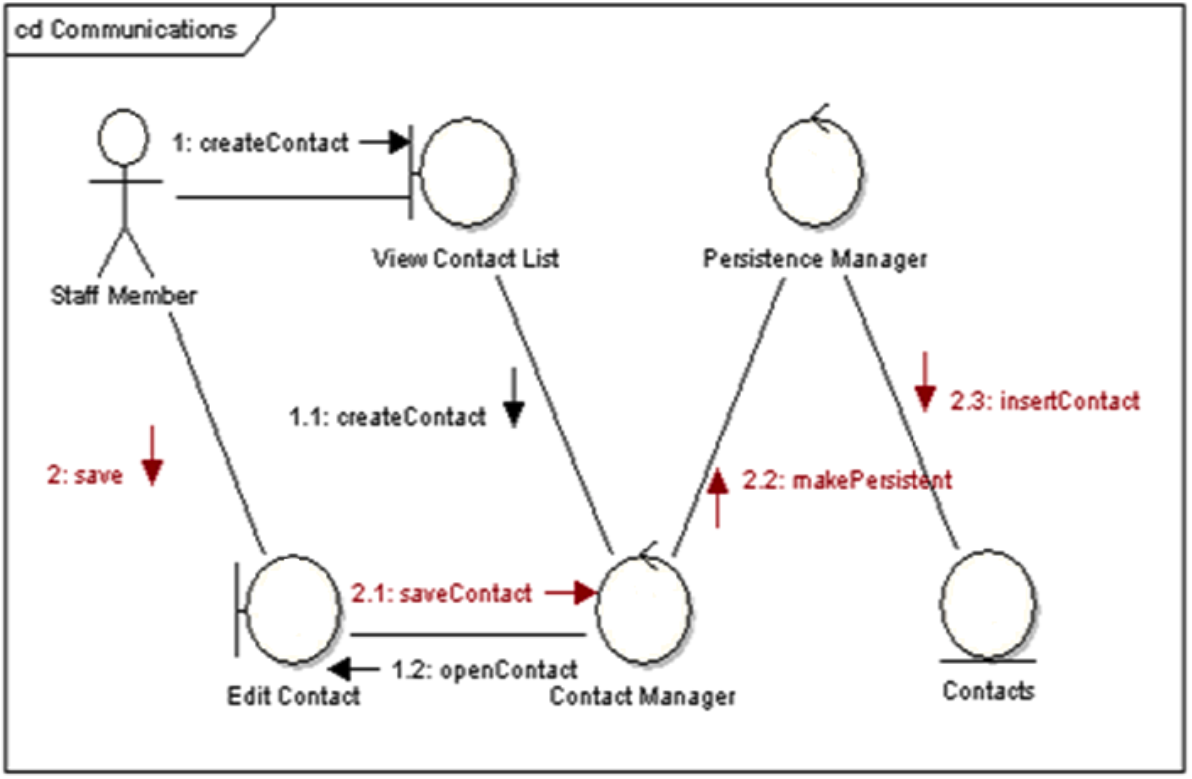
\includegraphics[width=0.4\linewidth]{res/teoria/Robustness.png}
    \caption{Robustness communication diagram}
\end{figure}
\section{T6 - Feasability and requirements elicitation}
Per ottenere le informazioni necessarie, dobbiamo identificare le fonti, acquisire le informazioni, analizzarle e verificarle. Infine, vanno sintetizzate. I vari stakeholder \textit{aka le persone interessate} possono essere così categorizzati con i loro interessi;
\begin{itemize}
    \item \textbf{Stakeholder}, interessato nel progetto
    \item \textbf{Developer}, alta produttività, mancanza di errori, minore sforzo possibile
    \item \textbf{Marketing sales}, soddisfazione del cliente e vendite
    \item \textbf{Project management}, budget, scadenze
    \item \textbf{Investor}, velocizzazione del processo
    \item \textbf{Customer and user}, usabilità e workflow
\end{itemize}
\subsection{Tecniche di elicitation}
\textit{(elicitation = tirare fuori le informazioni)}
\subsubsection{Document analysis}
Bisogna preparare i documenti che possono essere adatti e rilevanti, studiarli, annotare informazioni ed elencare le domande al riguardo. Infine, assieme agli stakeholder, verificare le note, organizzare i requirement e rispondere alle suddette domande. Questa tecnica può essere sfruttata quando non c'è presenza degli stakeholder, o per il cross-checking.
\subsubsection{Observation of the work environment}
L'obiettivo è determinare \textbf{chi, cosa, dove, quando, perché e come.} Bisogna ottenere il permesso dai supervisori, informare gli osservati, prendere appunti, evitare di disturbare ma al tempo stesso non dare nulla per scontato. I dati ottenuti sono molto affidabili.
\subsubsection{Questionario}
Serve determinare i fatti e le opinioni necessarie, in secundis, da chi reperirli. Determinare quindi le domande, aperte o chiuse, da fare. Può essere conveniente "testare" il questionario su un gruppo piccolo, per poi metterlo a posto e presentarlo a tutti. Questa tecnica restituisce molti dati, è facile da attuare ed affidabile. Non c'è però interazione, e si rischiano risposte incomplete. 
\subsubsection{Interviste}
Bisogna, prima di tutto, decidere chi intervistare. In seguito, preparare le domande e porle all'intervistato, con un linguaggio chiaro. Conviene prendere appunti e memo. Questo è un metodo ottimo perché permette di verificare i fatti, coinvolgendo gli end user. Non è però adatto a comprendere i domain requirements.
\subsubsection{Scenarios and use cases}
Essi sono esempi IRL di come il sistema verrà usato, basati su situazioni reali su cui gli stakeholder hanno senz'altro qualcosa da dire. Gli \textbf{scenari} sono semplicemente forme strutturare di user stories. Per gli use cases usiamo UML. Queste tecniche sono semplici ed utili, anche per sistemi complessi. È però difficile capire quando fermarsi, e soprattutto non sono utili a capire i \textbf{non-functional requirements.}
\subsection{Attività di supporto all'elicitation}
\subsubsection{Brainstorming}
Composto di due fasi, la prima di \textbf{storm} in cui si generano le idee, la seconda \textbf{calm} in cui vengono filtrate. Necessari due ruoli chiave: uno \textbf{scribe} ed un \textbf{moderatore}.
Nel filtraggio delle idee è fondamentale: unire idee simili, applicare i criteri di accettabilità, votare con una soglia o votare con dei \textit{campaign speeches.}
\subsubsection{Focus group}
Concetto simile al brainstorming ma più strutturato, esplora pro e contro di determinate opzioni. Fondamentale un moderatore.
\subsubsection{Prototypes}
Si mostra l'esecuzione di una task, si identificano le alternative, si cerca di estrapolare i possibili problemi. 
\section{T7 - Use Cases}
Gli \textbf{use case} sono scenari che sfruttano diagrammi UML, descrivono le task del sistema e l'interazione con gli attori. Non sono mappati one-to-one coi requirements, ma ogni requirement deve essere coperto da almeno uno use case. Gli use case sono quindi composti da use case diagrams, descrizioni testuali, ed interaction diagrams (opzionali).
Per identificare gli actor bisogna definire prima i boundary, poi gli utenti, l'hardware, i ruoli. Per identificare gli use case bisogna prima identificare il dominio. Vanno poi annotati come verbi rappresentanti le azioni. Per l'identificazione degli scenari, bisogna comprendere la situazione iniziale e il flusso di eventi. È utile capire cosa può andare male, e tutti i flussi alternativi. Infine, consideriamo la situazione finale. Uno use case deve avere un singolo attore iniziante, pochi step, non deve includere scelte implementative, può includere UML. Bisogna poi dare una priorità ai vari use case, in base all'impatto, la difficoltà, la necessità. 
\subsection{Componenti principali}
Uno use case deve definire lo stato iniziale e le precondizioni. Deve definire l'ordine degli eventi, le alternative, le situazioni eccezionali, e i risultati. Deve inoltre menzionare gli attori coinvolti, i diagrammi related, i problemi di design. Alcune guidelines:
\begin{itemize}
    \item Non pensare al lato implementativo
    \item Essere narrativi
    \item Elencare gli scenari funzionanti
    \item Elencare tutti i possibili use case
    \item Utilizzare un formato standard
    \item Utilizzare i verbi appropriati
    \item Documentare le situazioni eccezionali
    \item Non rappresentare singoli step come use cases
\end{itemize}
\begin{figure}[H]
    \centering
    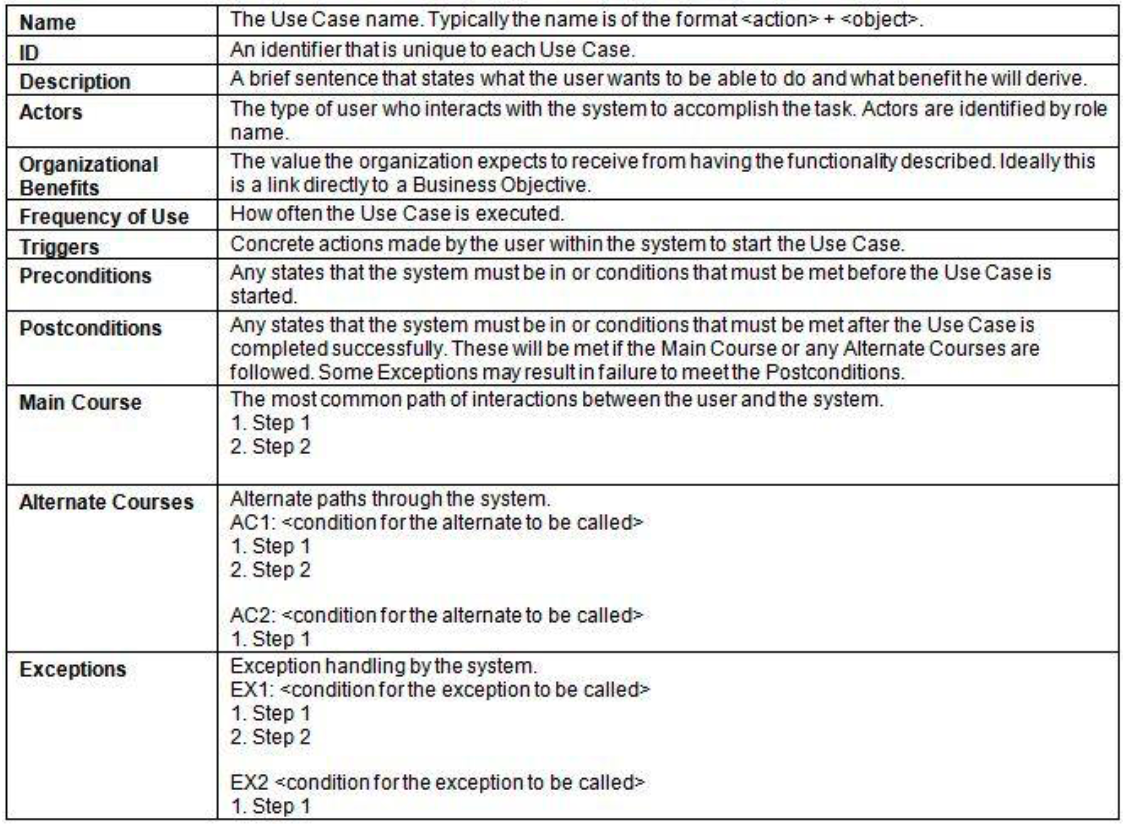
\includegraphics[width=0.8\linewidth]{res/teoria/UseCaseTemplate.png}
    \caption{Use case template}
\end{figure}

\section{T8 - Requirements Analysis}
L'analisi dei requirements raffina e struttura i requisiti in modo da renderli più chiari, precisi e formali. Esso definisce l'\textit{analysis model}, che raffina la descrizione informale dei requirement e la converte in diagrammi di flusso. Il suddetto non è un modello di design, ed è indipendente dalla piattaforma. Descrive le funzionalità che il sistema deve realizzare. 
\subsection{Analysis Classes}
Il concetto è quello di astrarre le entità del problema. Bisogna gestire i functional requirements (i non-functional sono gestiti nel \textbf{design architetturale}). Incorpora un set minimale di \textbf{responsabilità}. Questa analisi è rappresentata con digrammi di classe.
\subsection{Classes discovering techniques}
Esistono diverse tecniche atte a scovare le classi coinvolte. Procediamo ad elencarne le più importanti.
\subsubsection{Noun verb analysis}
Questa analisi sfrutta i documenti contenenti le specifiche di progetto, cercandovi nomi e verbi. Pare ovvio che la completezza dei documenti è fondamentale. La qualità dipende anche dallo stile di scrittura dei requisiti. 
\subsubsection{Use case driven approach}
Questo approccio sfrutta gli scenari di use case, e dipende quindi dalla correttezza dei suddetti. 
\subsubsection{Common Class Patterns}
Quest'analisi si basa sulla teoria della \textbf{classificazione generica degli oggetti}. Essa fornisce delle linee guida, ma non un processo sistematico atto ad ottenere le classi. Porta diversi rischi, tra cui quello di possibili interpretazioni errate dei nomi. 
\begin{figure}[H]
    \centering
    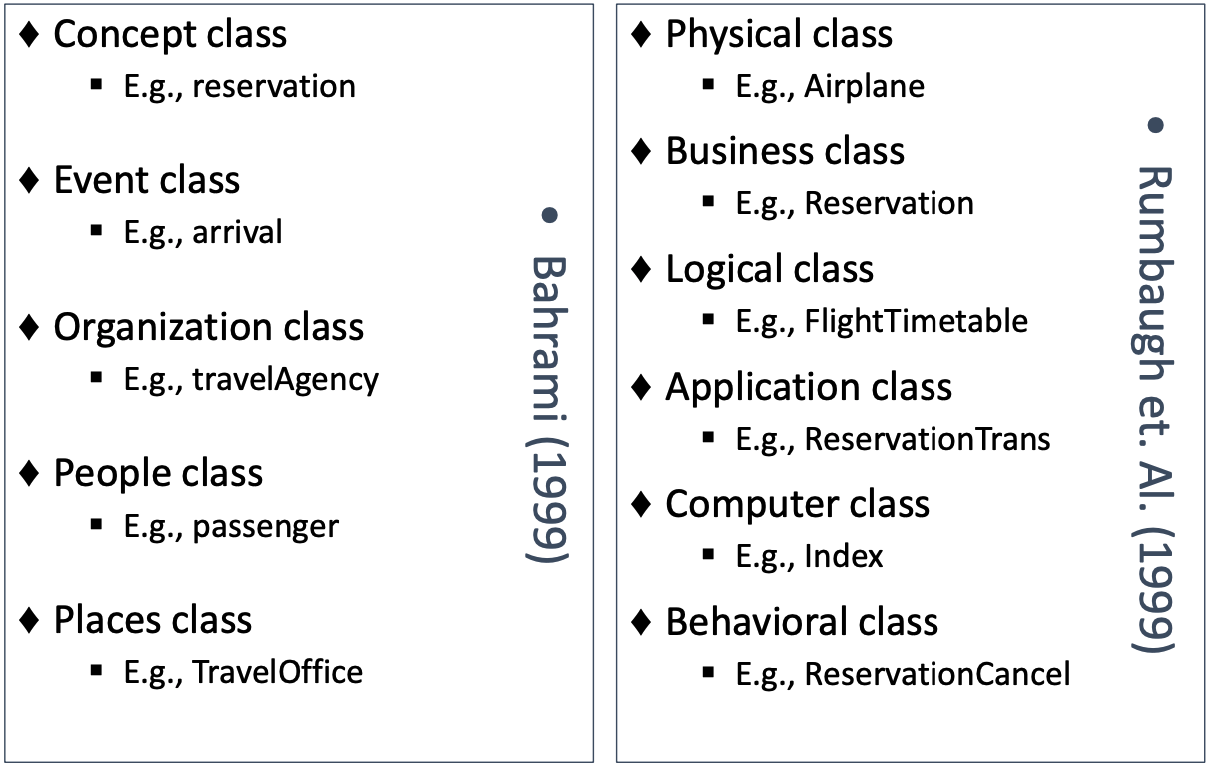
\includegraphics[width=\linewidth]{res/teoria/CommonClassPatterns.png}
    \caption{Common Class Patterns}
\end{figure}
\subsubsection{CRC Cards}
Le \textbf{CRC Cards} sono utilizzate in specifiche sessioni di brainstorming. Generalmente si parte dagli use cases, e si creano delle card con:
\begin{itemize}
    \item Class name
    \item Responsibilities
    \item Collaborators
\end{itemize}
Non viene fornito un metodo sistematico, e per questo le CRC cards sono piuttosto un mezzo di validazione dei requirements. 
\begin{figure}[H]
    \centering
    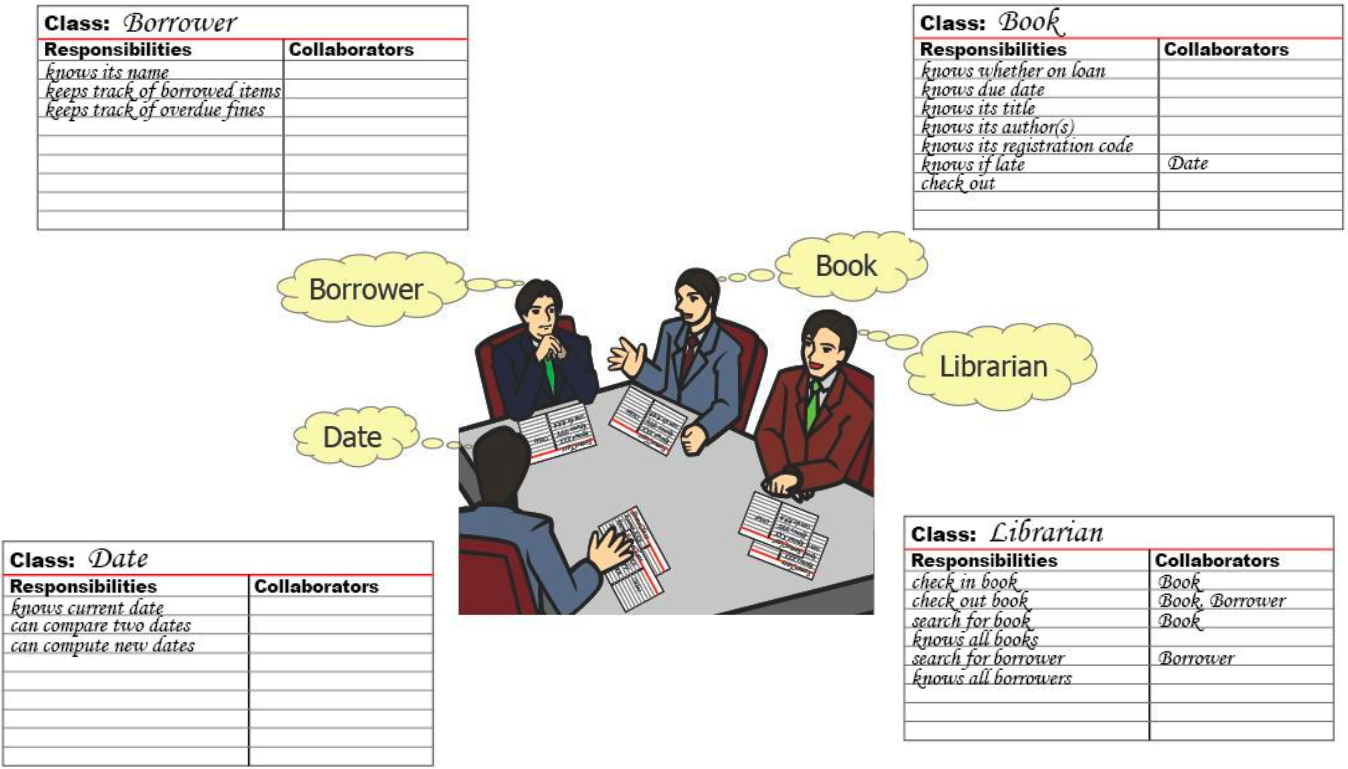
\includegraphics[width=\linewidth]{res/teoria/CRCCards.png}
    \caption{CRC Cards}
\end{figure}
Gli achievement di questo metodo sono:
\begin{itemize}
    \item Verificare la correttezza dello use case
    \item Verificare la correttezza delle associazioni
    \item Verificare la correttezza delle generalizzazioni
    \item Trovare le classi omesse
    \item Scovare opportunità di refactor
\end{itemize}
\subsection{Mixed approach}
Come sempre, la via di mezzo è quella vincente:
\begin{enumerate}
    \item Le classi iniziali provengono dalla conoscenza del dominio
    \item Si sfrutta, come guida, il common class pattern
    \item Per aggiungere altre classi, noun verb analysis
    \item Per verificare il lavoro, Use Case approach
    \item Per il brainstorming, CRC
\end{enumerate}
\section{T9 - Requirements Validation and Management}
\subsection{Validation}
La validazione consiste nel verificare la correttezza dei requirement, con due obiettivi principali: \textbf{completezza} e \textbf{costi}. Inoltre:
\begin{itemize}
    \item \textbf{Consistency}: assenza di conflitti
    \item \textbf{Realism}: possono essere effettivamente implementati?
    \item \textbf{Verifiability}: possono essere verificati?
\end{itemize}
La review dei requirement dovrebbe essere svolta continuamente durante la loro stesura. Essa deve essere svolta sia dal progettista che dal cliente. Alcuni issue da verificare sono:
\begin{itemize}
    \item Verifiability: il requirement è testabile?
    \item Comprehensibility: il requirement è stato compreso correttamente?
    \item Traceability: l'origine del requirement è chiara?
    \item Adaptability: i requirement possono essere cambiati senza impatti sul resto?
\end{itemize}
\begin{figure}[H]
    \centering
    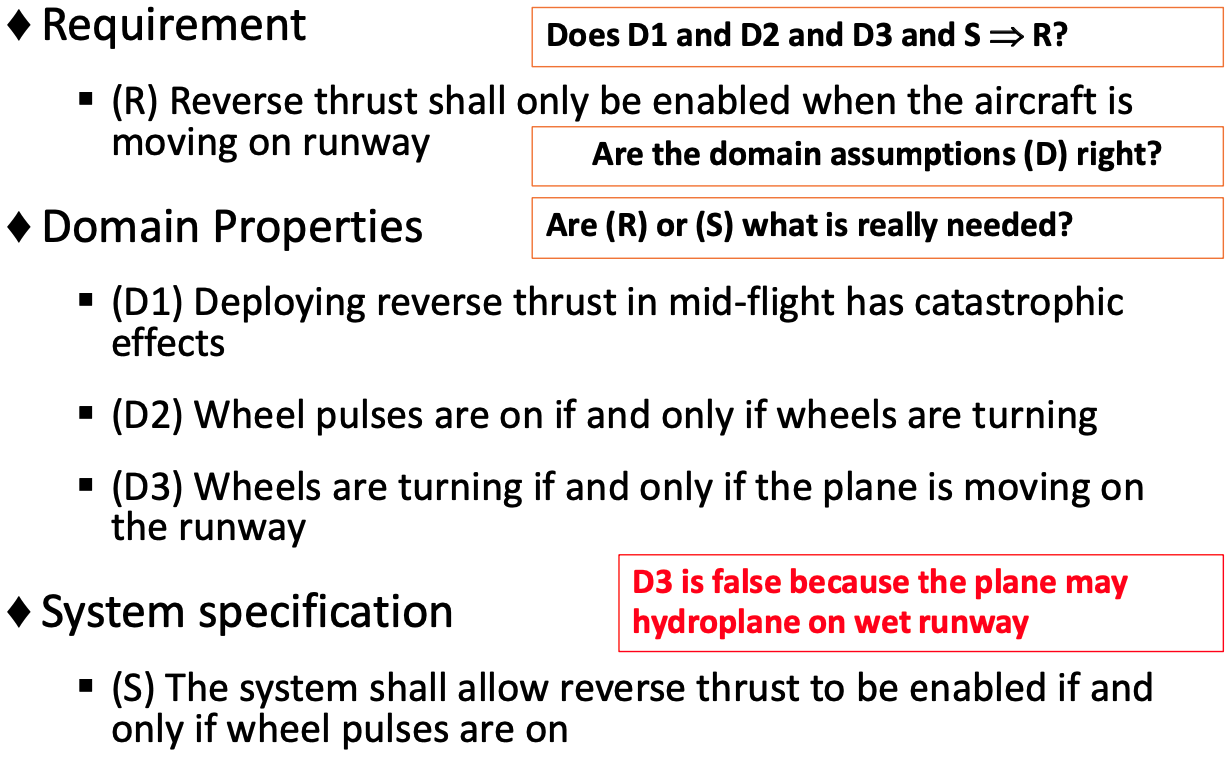
\includegraphics[width=\linewidth]{res/teoria/RequirementReview.png}
    \caption{Esempio di requirement review}
\end{figure}
\subsection{Requirements management}
Si verificano errori, conflitti ed inconsistenze. Vanno tenuti in conto i lati tecnici, la schedule, i costi, seguendo le priorità del cliente. 
Va quindi stimato il costo del progetto, controllata la requirements \gls{volatility}, negoziati i cambiamenti, ri-stimati i costi. L'interesse è soddisfare il cliente, rimanendo nel budget. 
Le necessità del requirement management sono:
\begin{itemize}
    \item Identificazione dei requirement
    \item Un processo di modifica
    \item Policy di tracciabilità
    \item Supporto del \gls{case}
\end{itemize}
\subsubsection{CASE tool support}
I requirement devono essere salvati in una zona sicura. Il change management deve essere un processo di workflow con passaggi definiti, e, se possibile, automatizzati. \textit{Immaginatelo come un Github Actions, ma nel '95.} Deve inoltre esserci un'automatizzazione dei link tra requirement, rinforzando la tracciabilità.
\subsubsection{Identificazione dei requirement}
I requirement devono essere identificati univocamente. Potremmo quindi numerare capitoli/sezioni, ma \textit{fa un po' schifo come approccio.} Per questo, sfruttiamo una numerazione dinamica, identificante i record nel DB. Potremmo sfruttare un'identificazione simbolica, con, ad esempio, sigle. \textit{Se usi degli issue tracker, è lo stesso concetto dei codici tra quadre.}
\subsubsection{Stati dei requirement}
I requirement possono avere degli stati (\textit{Anche qui, aver usato issue tracker può chiarire il concetto}):
\begin{itemize}
    \item Proposed
    \item Approved
    \item Rejected
    \item Implemented
    \item Verified 
    \item Deleted
\end{itemize}
\subsubsection{Change management}
È una buona idea implementare un version control dei requirement, per poter tracciare i cambiamenti. Prima di modificare un requirement, è importante analizzare il problema, i costi, e le specifiche. 
\begin{figure}[H]
    \centering
    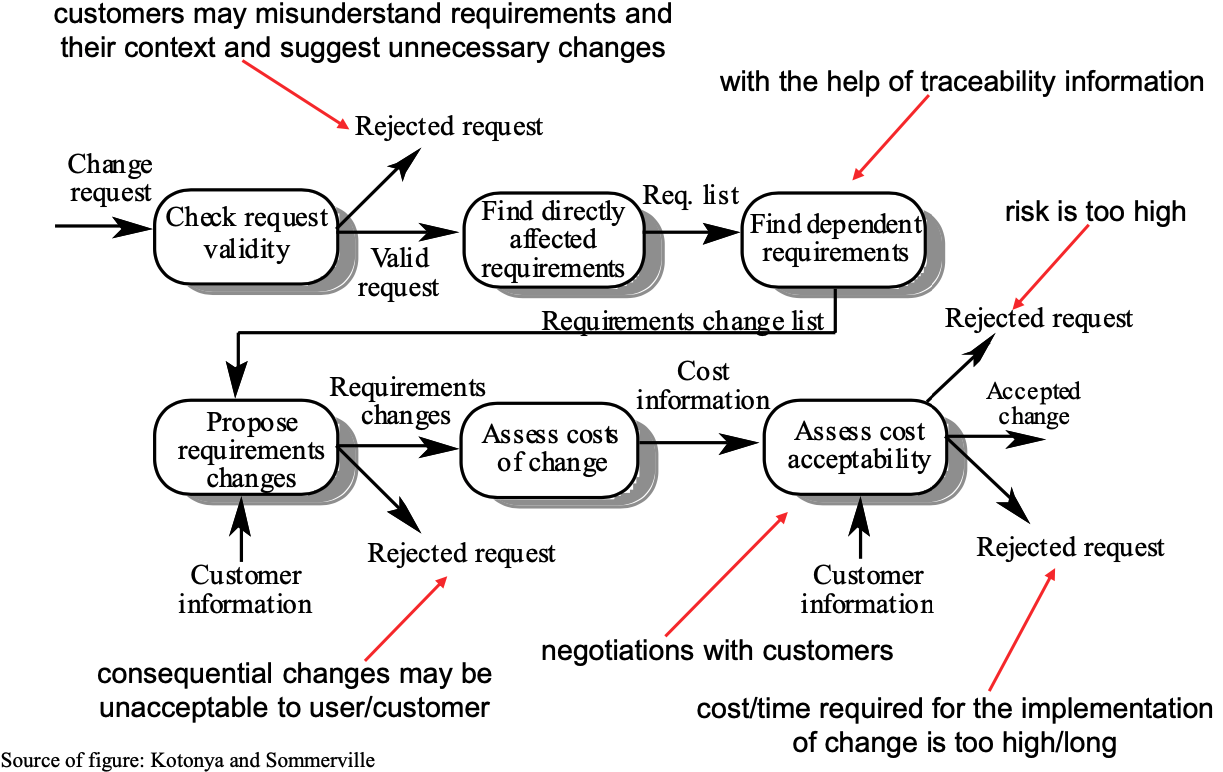
\includegraphics[width=\linewidth]{res/teoria/ChangeManagement.png}
    \caption{Change management diagram}
\end{figure}
\subsection{Traceability}
Lo sviluppo produce relazioni: predecessore-successore, master-subordinate. È fondamentale identificare queste relazioni ed il loro grado, allo scopo di tenere traccia dei \textit{path} nelle gerarchie. Alcuni esempi di traceability:
\begin{itemize}
    \item User needs $\rightarrow$ Product features
    \item Requirements $\rightarrow$ Implementation
    \item Use case $\rightarrow$ Test case
\end{itemize}
Distinguiamo tra vari tipi di traceability:
\begin{itemize}
    \item \textbf{Source}: la persona o il documento che hanno richiesto il requirement
    \item \textbf{Rationale}: fonte delle informazioni che descrivono le motivazioni del requirement
    \item \textbf{Requirements}: alcuni requirement sono collegati ad altri, da cui dipendono
    \item \textbf{Architecture}: collega i requirement ai sottosistemi in cui sono implementati
    \item \textbf{Design}: collega i requirement con specifici software/hardware necessari all'implementazione
    \item \textbf{Interface}: collega l'interfaccia di sistemi esterni che hanno reso necessario il requirement
    \item \textbf{Feature}: collega il requirement ai suoi componenti
    \item \textbf{Tests}: collega il requirement ai test cases che lo verificano
    \item \textbf{Code}: generalmente non stabilito direttamente, ma può essere implicato
\end{itemize}
Nella tracciabilità, si può incappare in diversi issue:
\begin{itemize}
    \item Gli stakeholder richiedono informazioni diverse
    \item Elevata quantità di informazioni richieste
    \item Problemi nel management manuale
    \item Necessità di tool specializzati
    \item Problemi di integrazione
\end{itemize}
\subsubsection{Traceability Planning}
Elementi fondamentali al planning sono:
\begin{itemize}
    \item Tipi di stakeholder
    \item Informazioni richieste
    \item Dove e da chi raccogliere informazioni
    \item Dove e come mantenere le informazioni 
    \item Dove e come cercare le informazioni
\end{itemize}
Abbiamo inoltre dei \glspl{constraint} al planning: 
\begin{itemize}
    \item \textbf{Numero di requirements}: maggiore è il numero di requirement, più sono necessarie delle policy formali di tracciabilità
    \item \textbf{Expected system lifetime}: in caso di lunghi tempi di vita, sono necessarie policy di tracciabilità più comprensive
    \item \textbf{Livello di maturità dell'organizzazione}: in organizzazioni con un'elevata maturità di processo vengono usate policy più dettagliate
    \item \textbf{Dimensioni di progetto e team}: maggiori le dimensioni, maggiore la formalità richiesta
    \item \textbf{Tipo di sistema}: sistemi critici come quelli real-time, o richiedenti sicurezza, hanno bisogno di policy di tracciabilità migliori
    \item \textbf{\Gls{constraint} addizionali del cliente}: il cliente può necessitare \gls{constraint} vari, ad esempio standard militari
\end{itemize}
\textit{I più svegli di voi si chiederanno perché passo dalla lezione 9 alla 12. La risposta è semplice, la 10 e la 11 sono dei doppioni di 8 e 9.}
\setcounter{section}{11}

\section{T12 - Object Constraint Language}
I diagrammi UML spesso non sono abbastanza raffinati per descrivere tutti i constraint sulle relazioni tra entità. Per questo, spesso, essi sono espressi tramite il linguaggio naturale, coi soliti problemi di ambiguità, o con un linguaggio formale, non comprensibile ai più. 
L'\textbf{Object Constraint Language} fa parte delle specifiche UML, ed è un linguaggio formale con sintassi e semantiche definite. Permette di descrivere espressioni e constraint tramite modelli object-oriented. È semplice da leggere e fu sviluppato da niente meno che \textbf{IBM}. Può essere utilizzato in vari modi:
\begin{itemize}
    \item Come query language
    \item Per specificare constraint su classi e tipi
    \item Per specificare constraint su operazioni
    \item Per specificare target su messaggi e azioni
    \item Per definire espressioni utili alla navigazione tra modelli UML
    \item Per testare requirement e specifiche
\end{itemize}
Definiamo tra 3 data types: quelli basic, quelli user-defined e le collection. È possibile eseguire operazioni booleane, operazioni reali/intere. Sono disponibili vari tipi di collection, tra cui nominiamo i set, gli ordered set, le bag \textit{(no, non quelle bag)}, in cui gli elementi possono essere ripetuti, e le sequenze, che sono bag ordinate.
Le collection hanno delle operazioni (le classiche operazioni da collection), come \code{size}, \code{isEmpty}, \code{notEmpty}, \code{sum}, \code{count}, \code{includes}, \code{includesAll}.
\subsection{Model types}
I \textbf{model types} sono classi, subclasses, classi di associazione, interfacce, enumerazioni. Hanno proprietà, come attributi, metodi, navigazioni (derivate dalle associazioni), enumerazioni. Possono essere inoltre \textit{referenziate} in espressioni OCL.
\subsection{Operazioni, espressioni, constraints}
Abbiamo alcune operazioni di base, come \code{oclIsTypeOf(type: OclType)}, o \code{oclIsKindOf}. Ogni espressione, contenente operazioni query, restituisce un risultato. Il tipo dell'espressione è il tipo del risultato. Un constraint è semplicemente un'espressione booleana. 
I constraint sono quindi restrizioni su uno o più valori di un modello/sistema object-oriented. Sono dichiarativi, non hanno \textit{side effects}, ed hanno sintesi formale e semantiche. Perché si usano?
\begin{itemize}
    \item Migliore documentazione
    \item Più precisione
    \item Comunicazione senza ambiguità
\end{itemize}
Abbiamo svariati tipi di constraint:
\begin{itemize}
    \item \textbf{Invariant}: deve essere vero quando l'istanza è a riposo
    \item \textbf{Pre-condition}: deve essere vero quando un'operazione è invocata
    \item \textbf{Post-condition}: deve essere vero dopo il completamento di un'operazione
    \item \textbf{Guard}: deve essere vero prima che una transazione possa accadere, quindi è una specie di pre-condition
\end{itemize}
La sintassi è semplice: \code{[termine del constraint][nome del constraint]:[espressione booleana]}. I termini per i constraint suddetti sono \code{inv}, \code{pre}, \code{post}, \code{pre/post…implies oclInState}.
\section{T13 - Design Process}
Il \textbf{design process} è il processo che permette di trovare come implementare il sistema, partendo dai requirements e tenendo conto dei \textbf{design general principles}. L'obiettivo è un \textbf{modello} ragionevole e realizzabile. 
\subsection{Linee guida}
\begin{itemize}
    \item Esibire un'organizzazione modulare che fa un uso intelligente di controllo tra i componenti
    \item Partizionare logicamente in componenti che realizzano compiti
    \item Descrivere sia dati, che procedure 
    \item Arrivare ad interfacce che riducono la complessità
    \item Derivare utilizzando un metodo ripetibile che fa uso delle informazioni dei requirements 
\end{itemize}
Un buon design deve implementare tutti i requirement espliciti del modello di analisi, e tutti quelli impliciti desiderati dal cliente. Dev'essere leggibile e comprensibile, sia per chi scrive codice, sia per chi lo testa e supporta. In generale, dovrebbe dare un'immagine generale del software, indicandone i dati, i domini funzionali e \textit{behavioral} dal punto di vista dell'implementazione. 
\subsection{Stadi del design process}
Il primo passo è la \textbf{comprensione del problema}, che richiede di osservare il problema da punti di vista differenti, per riconoscere i design requirements. Il secondo è \textbf{identificare una o più soluzioni}, valutando quelle possibili e scegliendo la più appropriata, in base all'esperienza del designer ed alle risorse disponibili. Il design process è un \textbf{processo iterativo ed incrementale}. 
\subsection{Design as series of decisions}
Il design può essere visto come una serie di decisioni, scomponendolo in più sottoproblemi, ognuno dei quali presentante diverse soluzioni, tra cui bisogna decidere. 
Alcuni tradeoff possono essere:
\begin{itemize}
    \item Funzionalità vs. Usabilità
    \item Costo vs. Robustezza 
    \item Efficienza vs. Portabilità 
    \item Velocità di sviluppo vs. Funzionalità 
    \item Costo vs. Riutilizzabilità 
    \item Compatibilità col vecchio vs. Leggibilità 
\end{itemize}

Gli step per le priority based decision sono:
\begin{enumerate}
    \item Elencare le alternative possibili
    \item Elencare i pro e i contro di ogni alternativa, rispetto agli obiettivi e alle priorità 
    \item Determinare se alcune alternative impediscono il raggiungimento degli obiettivi 
    \item Scegliere l'alternativa che permette di coprire più obiettivi 
    \item Aggiustare le priorità per le decisioni future
\end{enumerate}
Alcuni strumenti utilizzabili durante questo processo sono la \textit{concept table}, la \textit{concept fan}, la \textit{decision matrix}.
\subsubsection{Approcci}
Abbiamo tre possibili tipi di approccio:
\begin{itemize}
    \item Approccio \textbf{top-down}: prima, si \textit{designa} la struttura di alto livello del sistema, poi si prendono le decisioni man mano più specifiche 
    \item Approccio \textbf{bottom-up}: qui, prima si decidono le utilities di basso livello riutilizzabili, poi il modo di integrarle insieme 
    \item Approccio \textbf{mixed}: si utilizza il \textit{top-down} per decidere la struttura, ed il \textit{bottom-up} per i componenti riutilizzabili 
\end{itemize}
\subsubsection{Attività, rischi e obiettivi}
Distinguiamo tre attività nel design:
\begin{itemize}
    \item Design dell'architettura, dove si decidono i sottosistemi ed i componenti e la loro interazione 
    \item User interface design 
    \item Component/class design, dove si decidono le strutture dati ed i meccanismi computazionali
\end{itemize}
Il design è però un'attività che richiede notevole esperienza, e pertanto un solo ingegnere non dovrebbe mai tentare il design di sistemi grandi, ma piuttosto studiare quelli di altri sistemi. Infatti, un cattivo design potrebbe portare a manutenzione costosa, mentre un buon design dovrebbe essere tenuto in conto per tutta la vita del software, in modo flessibile, documentato, e con una buona gestione delle modifiche. 
In conclusione, un buon design è \textbf{flessibile}, \textbf{dettagliato al punto giusto}, \textbf{ben documentato}, e con \textbf{un buon change management}.
\section{T14 - Design concepts}
Un sistema software ha diversi, possibili, problemi: 
\begin{itemize}
    \item \textbf{Rigidità}: quando il codice è difficile da cambiare, il management è riluttante al cambiamento 
    \item \textbf{Fragilità}: quando anche cambiamenti minimali creano effetti a cascata, rompendo il codice in punti inaspettati 
    \item \textbf{Immobilità}: il codice è così intricato da rendere impossibile il riutilizzo di componenti, che sarebbe più costoso della realizzazione da zero
    \item \textbf{Viscosità}: molto più semplice l'hack del mantenimento del design originale
\end{itemize}
\subsection{Software design concepts}
\subsubsection{Abstraction}
L'\textbf{astrazione} permette di focalizzarsi su aspetti importanti di un problema ad un livello particolare, senza l'offuscamento dovuto a dettagli non importanti. Permette la descrizione di un sistema come struttura a livelli 
\subsubsection{Refinement} 
Il raffinamento \textit{(?)} è un processo top-down dove, in ogni passo, una o più istruzioni sono decomposte in istruzioni più dettagliate, partendo da una specifica di alto livello e dividendola in sottoproblemi ricorsivamente, finché i sottoproblemi non hanno soluzioni immediate. Questo non è appropriato per sistemi di larga scala o distribuiti, ma piuttosto per il design di metodi. 
\subsubsection{Information hiding}
Il design richiede una serie di decisioni, e per ognuna di queste, dobbiamo chiederci chi deve sapere e chi no. L'information hiding è strettamente legato a:
\begin{itemize}
    \item \textbf{Abstraction}: se qualcosa è nascosto, l'utente può astrarre da quell'informazione \textit{Scusate.}
    \item \textbf{Coupling}: un segreto diminuisce il coupling tra un modulo ed il suo environment 
    \item \textbf{Cohesion}: il segreto è ciò che unisce le parti del modulo 
\end{itemize}
\subsubsection{Modularity}
La modularità è basata sull'integrazione di componenti separati in moduli, per risolvere requirements di problemi. 
È basata sull'uso di unità linguistiche modulari, poche interfacce semplici ed esplicite, offuscamento delle informazioni. Un metodo di design può essere detto modulare solo se supporta:
\begin{itemize}
    \item \textbf{Decomposability}: un problema software può essere diviso in un piccolo numero di piccoli sottoproblemi connessi da una struttura semplice, ed abbastanza indipendenti da permettere lavoro separato su ogni componente. 
    \item \textbf{Composability}: alcuni elementi software possono essere combinati tra loro per produrre nuovi sistemi, possibilmente in ambienti diversi da quello di sviluppo 
    \item \textbf{Understandability}: un lettore umano può comprendere ogni modulo senza dover conoscere gli altri, o conoscerne una minima parte 
    \item \textbf{Continuity}: una piccola modifica nella specifica modificherà un solo modulo, o una minima parte 
    \item \textbf{Protection}: l'effetto di una condizione anormale durante l'esecuzione coinvolgerà un solo modulo, o verrà propagata ad una minima parte 
\end{itemize}
I principi per il design modulare sono: \textbf{linguistic modular units} (i moduli devono corrispondere alle unità del linguaggio, come pacchetti o moduli), \textbf{poche interfacce}, \textbf{poco scambio di informazioni tra moduli}, \textbf{interfacce esplicite} (se due moduli comunicano, dev'essere ovvio), \textbf{information hiding}(tutte le informazioni di un modulo dovrebbero essere private, se non specificatamente dichiarato il contrario, e per l'accesso bisogna utilizzare interfacce). 
\subsubsection{Cohesion}
La coesione misura la \textit{chiusura} di una relazione tra elementi di un componente/classe. Una coesione forte è desiderabile perché semplifica le correzioni, le modifiche, le estensioni, riduce il testing e promuove il riutilizzo. 
Abbiamo più livelli di coesione (dal più basso al più alto):
\begin{itemize}
    \item \textbf{Coincidental}: gli elementi non hanno relazioni ma sono uniti per convenienza
    \item \textbf{Logical}: elementi che svolgono funzioni simili (input simile, error handling)
    \item \textbf{Temporal}: elementi che sono attivati allo stesso tempo e hanno avvio e fine comuni 
    \item \textbf{Procedural}: elementi che compongono una singola sequenza di controllo 
    \item \textbf{Communicational}: elementi che operano sullo stesso input o producono lo stesso output
    \item \textbf{Sequential}: elementi che condividono o operano sugli stessi dati (l'output di uno è l'input dell'altro)
    \item \textbf{Functional}: elementi che sopperiscono a un singolo functional requirement
    \item \textbf{Object}: solo operazioni tra oggetti permettono modifiche o ispezioni agli oggetti 
\end{itemize}
\subsubsection{Coupling}
Misura l'interconnessione tra moduli. Quando è debole, i moduli sono fortemente indipendenti. Livelli di coupling dal più debole al più forte:
\begin{itemize}
    \item \textbf{No direct}: nessuna dipendenza
    \item \textbf{Data}: solo i dati necessari sono passati come argomenti
    \item \textbf{Stamp}: le strutture dati sono passate per lista di argomenti e solo una parte è utilizzata 
    \item \textbf{Control}: si interfaccia passando flags e altri parametri 
    \item \textbf{External}: è legato a device o device drivers
    \item \textbf{Premature}: utilizza numeri o altri valori attraverso il programma 
    \item \textbf{Content}: modifica gli statement/dati dell'altro modulo o si ramifica nel mezzo di un modulo
\end{itemize}
Il tradeoff qui è:
\begin{itemize}
    \item \textbf{Coupling elevato}: i componenti sono difficili da comprendere autonomamente, le modifiche causano problemi negli altri moduli, il riutilizzo è scoraggiato. In compenso, migliori performance 
    \item \textbf{Coupling ridotto}: aumenta i costi in performance, ma è più veloce da sviluppare e mantenere.
\end{itemize}
\section{T15 - Object oriented design principles}
Illustriamo in questa lezione i principi \textbf{SOLID}.
\subsection{Principi dell'Object-Oriented Design}
\subsubsection{SRP - Single Responsibility Principle}
Il principio di singola responsabilità afferma che una classe deve avere una sola ragione di cambiare. Le modifiche ai requirements solitamente si mappano sulle responsabilità. Più responsabilità equivalgono a più probabilità di cambiare. Le responsabilità nella stessa classe sono coupled.
Tante classi con responsabilità distinte equivalgono a un design più flessibile. 
\begin{center}
    \textit{In programming, the Single Responsibility Principle states that every module or class should have responsibility over a single part of the functionality provided by the software.}
\end{center}
\subsubsection{OCP - Open Closed Principle}
Un modulo o componente dev'essere \textbf{aperto verso l'estensione}, ma \textbf{chiuso verso la modifica}. In questo modo, si possono aggiungere nuovi comportamenti, ma le modifiche non sono richieste. Ogni modifica può introdurre bug e richiede lavoro addizionale. Al contrario, scrivere nuove classi più difficilmente genera problemi. 
\begin{center}
    \textit{In programming, the open/closed principle states that software entities (classes, modules, functions, etc.) should be open for extensions, but closed for modification.
    If you have a general understanding of OOP, you probably already know about polymorphism. We can make sure that our code is compliant with the open/closed principle by utilizing inheritance and/or implementing interfaces that enable classes to polymorphically substitute for each other.}
\end{center}
\subsubsection{Liskov Substitution Principle}
Le subclasses dovrebbero essere sostituibili dalle loro base classes: le classi derivate devono onorare i contratti delle loro classi base, estendendone le funzionalità senza modificarle. Altrimenti, le classi derivate producono effetti indesiderati quando usate con moduli esistenti. 
\begin{center}
    \textit{More generally it states that objects in a program should be replaceable with instances of their subtypes without altering the correctness of that program.}
\end{center}
\subsubsection{ISP - Interface Segregation Principle}
Avere multiple interfacce client-specific è molto meglio di averne una generica. In questo modo, le interfacce sono semplici e focalizzate. Per questo è consigliabile un refactor delle interfacce grandi in più sottointerfacce, in modo da non forzare il client a dipendere da cose di cui non ha bisogno. 
\begin{center}
    \textit{In programming, the interface segregation principle states that no client should be forced to depend on methods it does not use.
    Put more simply: Do not add additional functionality to an existing interface by adding new methods.
    Instead, create a new interface and let your class implement multiple interfaces if needed.}
\end{center}
\subsubsection{DIP - Dependency Inversion Principle}
I moduli di alto livello non dovrebbero dipendere da moduli di basso livello. Entrambi dovrebbero dipendere da astrazioni. Le astrazioni non devono dipendere da dettagli, ma i dettagli dovrebbero dipendere da astrazioni. Bisognerebbe inoltre evitare di derivare, associare o dipendere da classi concrete o componenti. 
\subsection{Principi di package cohesion}
\subsubsection{REP - Release/Reuse Equivalency Principle}
L'unità di riuso è l'unità di release: il codice non dovrebbe essere riutilizzato ricopiandolo e incollandolo. In questo modo, una modifica alla libreria originale verrebbe persa. Invece, il codice dovrebbe essere inserito tramite una release della libreria, in modo da poterla mantenere aggiornata. Un pacchetto costituito da classi riutilizzabili è più utile e riutilizzabile a sua volta. Pacchetti che non c'entrano nulla non dovrebbero essere inclusi. 
\subsubsection{CCP - Common Closure Principle}
Le classi che cambiano insieme, devono stare insieme: questo minimizza l'impatto delle modifiche. Le classi dovrebbero essere \textit{packaged} con coesione, indirizzando la stessa area funzionale o comportamentale, ed essendo inseparabili ed interdipendenti. 
\subsubsection{CRP - Common Reuse Principle}
Le classi che non sono riutilizzabili insieme non dovrebbero essere raggruppate, quelle raggruppate dovrebbero cambiare per gli stessi motivi. 
\subsection{Package Coupling Principles}
\subsubsection{ADP - Acyclic Dependencies Principle}
Non bisogna permettere cicli nel grafico delle dipendenze. Non bisogna interferire con i programmatori. \textit{Sono gente cattiva.}
\subsubsection{SDP - Stable Dependencies Principle}
Le dipendenze tra componenti dovrebbero essere nella direzione della stabilità: un componente deve dipendere solo da componenti più stabili. Ogni volta che un pacchetto cambia, tutti i pacchetti che ne dipendono devono essere validati per assicurare che lavorino correttamente dopo la modifica. Più pacchetti dipendono da un pacchetto instabile, più grande è il danno quando cambia.
\subsubsection{SAP - Stable Abstractions Principle}
Un pacchetto dev'essere tanto più astratto quanto è stabile. I pacchetti astratti dovrebbero essere responsabili e indipendenti, quelli concreti irresponsabili e dipendenti. Un'architettura ideale ha la seguente struttura: pacchetti instabili in cima, pacchetti stabili alla base. 
\subsection{Attività per un buon design}
\begin{itemize}
    \item \textbf{Dividi e conquista}: avere a che fare con qualcosa di grande tutto in una volta è molto più difficile di avere a che fare coi sottoproblemi. 
    \item \textbf{Aumentare la coesione} quando possibile: un sistema con alta coesione tiene insieme cose che devono stare insieme e tiene fuori il resto
    \item \textbf{Ridurre il coupling}, ossia le interdipendenze tra moduli
    \item \textbf{Aumentare l'astrazione} il più possibile, allo scopo di nascondere i dettagli e ridurre la complessità
    \item \textbf{Aumentare la riutilizzabilità} quando possibile
    \item \textbf{Riutilizzare design e codice esistenti}
    \item Pensare alla \textbf{flessibilità}: anticipare le modifiche future è un buon investimento a lungo termine
    \item \textbf{Anticipare l'obsolescenza}: pianificare modifiche nella tecnologia o nell'environment del futuro 
    \item Pensare alla \textbf{portabilità}
    \item Pensare alla \textbf{testabilità}
    \item Rimanere sempre sulla \textbf{difensiva}: non sappiamo mai se l'utente farà davvero ciò che deve.
\end{itemize}
\section{T16 - Design Patterns}
\textit{Si, hai letto bene. Sei fottuto. \textbf{Cominciamo.}}
La modellazione richiede di superare i nostri limiti mentali; un buon modello lo fa: è facile da ricordare, poco complesso, astratto, strutturato. Per comunicare un modello utilizziamo la navigazione e la riduzione di complessità, partendo da un modello molto semplice decorato di mano in mano. Per ridurre la complessità, cerchiamo ereditarietà e patterns. Nel OOP abbiamo strutture ricorrenti che promuovono astrazione, flessibilità, modularità, eleganza. Queste strutture sono un'importante conoscenza per lo sviluppo di ogni tipo di sistema, il problema è trovare il modo giusto di esprimerle. 
Un \textbf{design pattern} è una soluzione ricorrente ad un problema comune, che può essere usata in modi diversi. È dipendente da linguaggio ed implementazione. I design patterns hanno vari obiettivi:
\begin{itemize}
    \item Codificare un buon design
    \item Dare nomi espliciti alle strutture
    \item Catturare e preservare le informazioni sul design 
    \item Facilitare la ristrutturazione/refactoring 
\end{itemize}
Abbiamo due forme possibili: \textbf{Alexandrian} e \textbf{GoF}.
\subsection{Creational Patterns}
I creational patterns permettono la creazione flessibile di oggetti per rendere il sistema indipendente dagli oggetti creati. Ogni famiglia e le classi istanziate possono essere conosciute solo a runtime. 
\subsubsection{Factory Method}
\paragraph{Scopo}
Il metodo Factory fornisce un'interfaccia per creare oggetti in una subclass, permettendole di modificare il tipo di oggetti creati.
\paragraph{Problema}
Immaginiamo di dover creare un'applicazione che gestisca un servizio di logistica. La prima versione utilizza solo trasporto su ruota, quindi la maggior parte del codice sta nella classe \code{Truck}. Dopo un po', l'app diventa popolare. Decidi di implementare anche il trasporto via mare. Aggiungere la classe \code{Ship} richiederebbe modifiche in tutto il codice. Aggiungerne altre, pure.
\paragraph{Soluzione}
Il metodo Factory permette di sostituire la creazione di nuovi oggetti (con \code{new}) con chiamate a un metodo factory. Gli oggetti generati da questo metodo sono detti \textbf{prodotti.} C'è un vincolo da rispettare: i prodotti devono implementare un'interfaccia comune.
\begin{figure}[H]
    \centering
    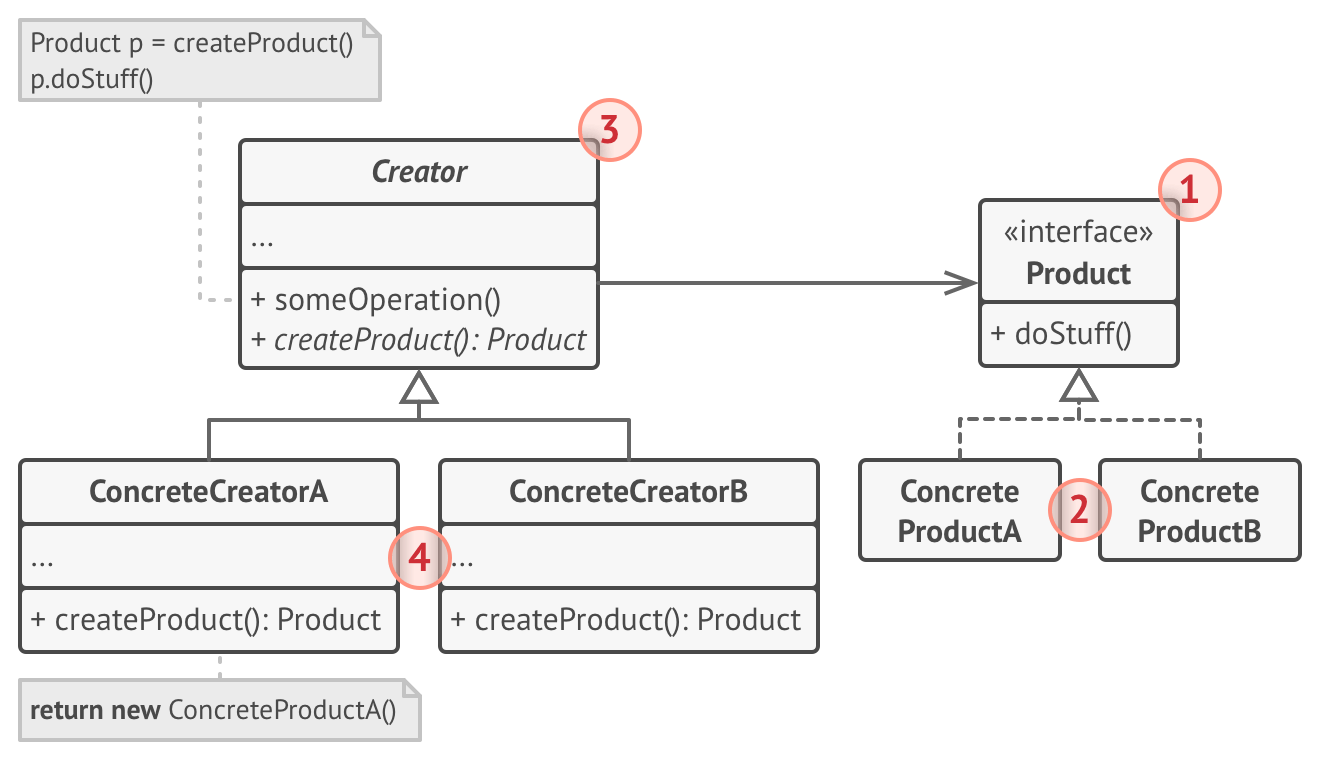
\includegraphics[width=\linewidth]{res/teoria/Factory.png}
    \caption{Esempio generico}
\end{figure}
\paragraph{Applicabilità}
\begin{itemize}
    \item Una classe non può anticipare la classe degli oggetti da creare
    \item Una classe delega responsabilità a delle helper subclasses
\end{itemize}
\subsubsection{Abstract Factory}
\paragraph{Scopo}
L'\textbf{abstract factory} permette di creare famiglie di oggetti related senza specificarne le classi concrete.
\paragraph{Problema}
Immaginiamo di voler creare un simulatore di negozio di arredamenti. Il codice consiste di classi rappresentanti 1) una famiglia di prodotti (sedia, divano, tavolo) 2) varianti di questa famiglia. 
Serve un modo di creare oggetti in modo da matcharli con altri arredamenti della stessa famiglia. Non vogliamo inoltre modificare il codice esistente quando aggiungiamo nuovi prodotti o famiglie. 
\paragraph{Soluzione}
Prima di tutto, dichiariamo le interfacce di ogni distinto prodotto, avendo come sottoclassi le varianti del suddetto. In secundis, dichiariamo l'abstract factory, un'interfaccia con una lista di metodi di creazione facenti parte di una famiglia di prodotti. Questi metodi ritornano prodotti astratti. A questo punto, estendiamo l'abstract factory con le factory concrete per ogni variante. 
\begin{figure}[H]
    \centering
    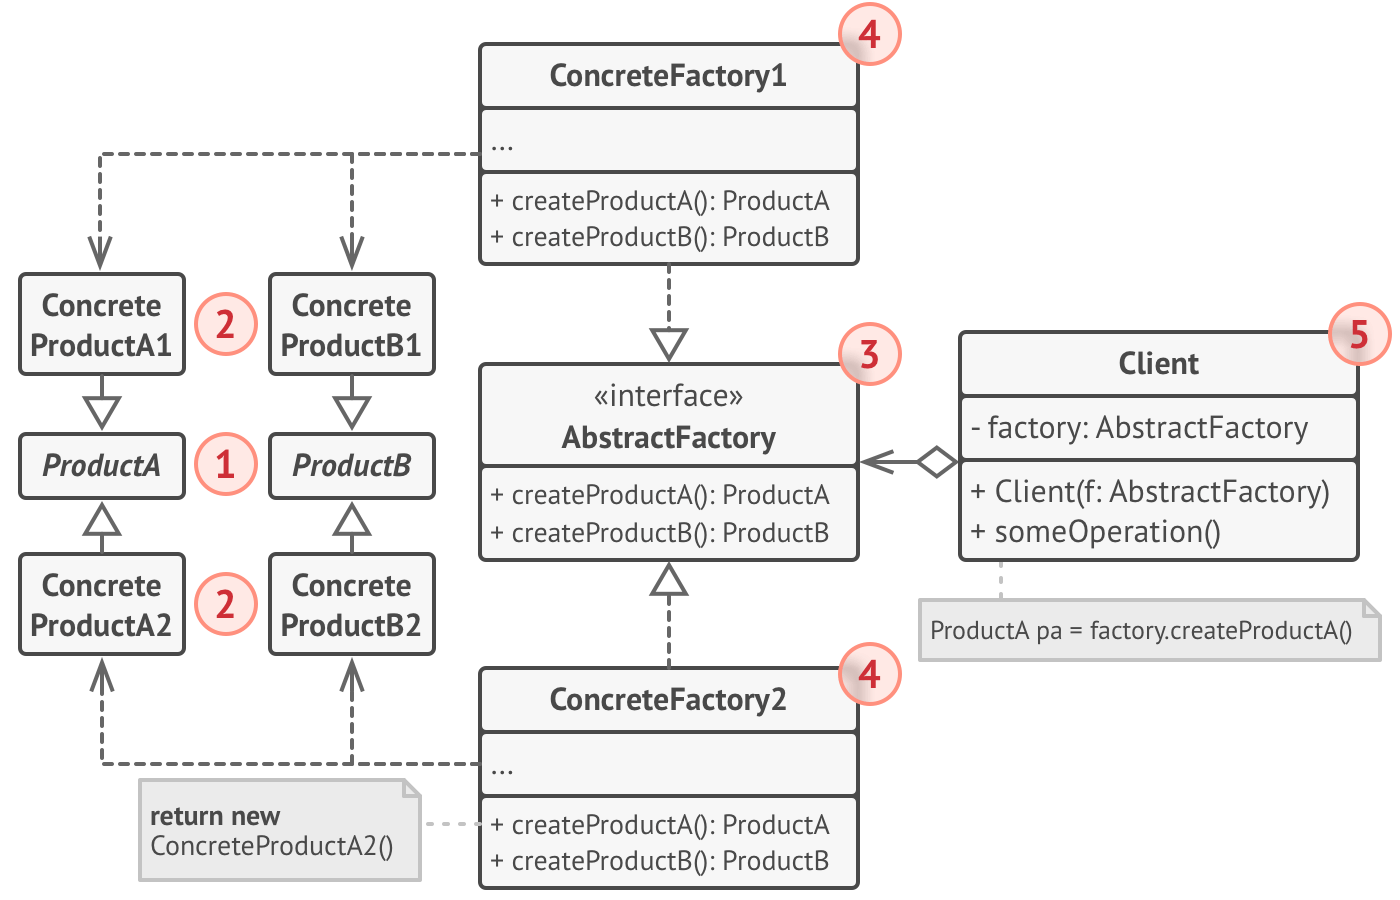
\includegraphics[width=\linewidth]{res/teoria/AbstractFactory.png}
    \caption{Struttura}
\end{figure}
\paragraph{Applicabilità}
Quando i client non possono anticipare gruppi di classi da istanziare.
\subsubsection{Builder}
\paragraph{Scopo}
Il \textbf{builder} permette di costruire oggetti un pezzo alla volta. Il pattern permette di produrre tipologie e rappresentazioni diverse di un oggetto, utilizzando lo stesso codice di costruzione.
\paragraph{Problema}
Immaginiamo un oggetto complesso che richiede inizializzazioni step-by-step di molti campi e oggetti annidati. Questo porterebbe ad un gigante costruttore con molti parametri. \textit{Bella merda.} Per esempio, se avessimo un oggetto \code{House}, dovremmo costruire 4 muri, installare una porta, le finestre, un tetto. Se volessimo però qualche caratteristica in più, come un garage, dovremmo inserire un boolean tipo \code{hasGarage} nel costruttore.
\paragraph{Soluzione}
Il builder pattern suggerisce di estrarre il codice di costruzione dell'oggetto fuori dalla sua classe, ad oggetti detti \textbf{builders.} Possiamo andare oltre e creare una classe che chiama gli step dei builder, detta \textbf{director}, che definisce l'ordine delle chiamate, mentre i builder si occupano dell'implementazione. 
Il director non è strettamente necessario.
\begin{figure}[H]
    \centering
    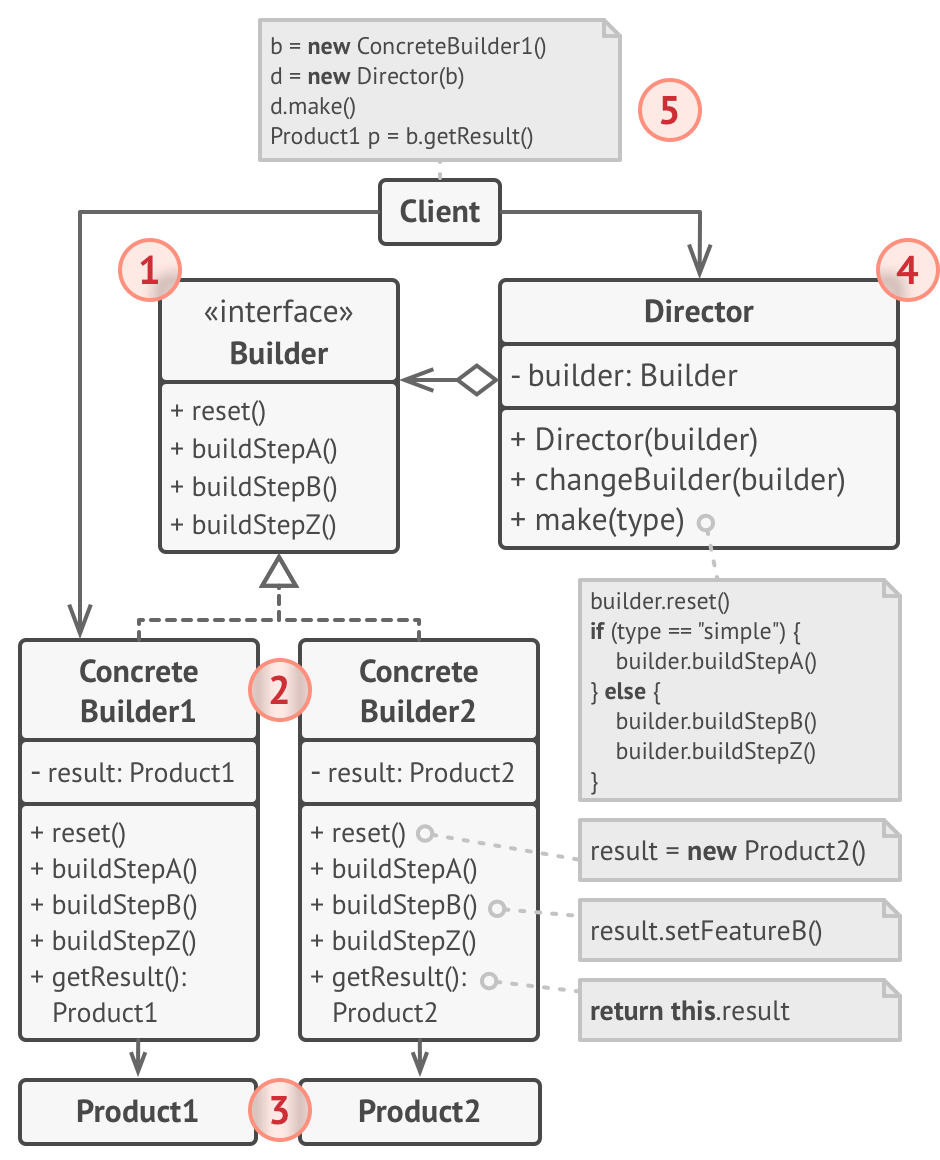
\includegraphics[width=\linewidth]{res/teoria/Builder.png}
    \caption{Struttura}
\end{figure}
\paragraph{Applicabilità}
Si applica quando l'algoritmo di creazione dell'oggetto deve essere indipendente dalle parti che lo compongono e come vengono assemblate. Insomma, quando il processo di costruzione deve permettere prodotti diversi.
\subsubsection{Prototype}
\paragraph{Scopo}
Il \textbf{prototype} permette di copiare oggetti esistenti senza dover rendere il codice dipendente dalla classe effettiva.
\paragraph{Problema}
Immaginiamo di avere un oggetto, e volerne creare una copia esatta. Come fare? Farlo dall'esterno non è ideale: ci perderemmo tutti i dati privati! Inoltre, per fare il duplicato dobbiamo conoscere la classe concreta dell'oggetto. \textit{Not stonks.}
\paragraph{Soluzione}
Il prototype pattern delega il processo di clonazione all'oggetto effettivo che stiamo copiando. Dichiariamo un'interfaccia comune, tipo \code{Clonable}, che contenga il metodo \code{clone()}. In questo modo, implementando il metodo \code{clone()} in tutte le classi (saranno metodi simili) abbiamo la possibilità di clonare oggetti. Un oggetto che supporta la clonazione è detto \textit{prototype.}
\begin{figure}[H]
    \centering
    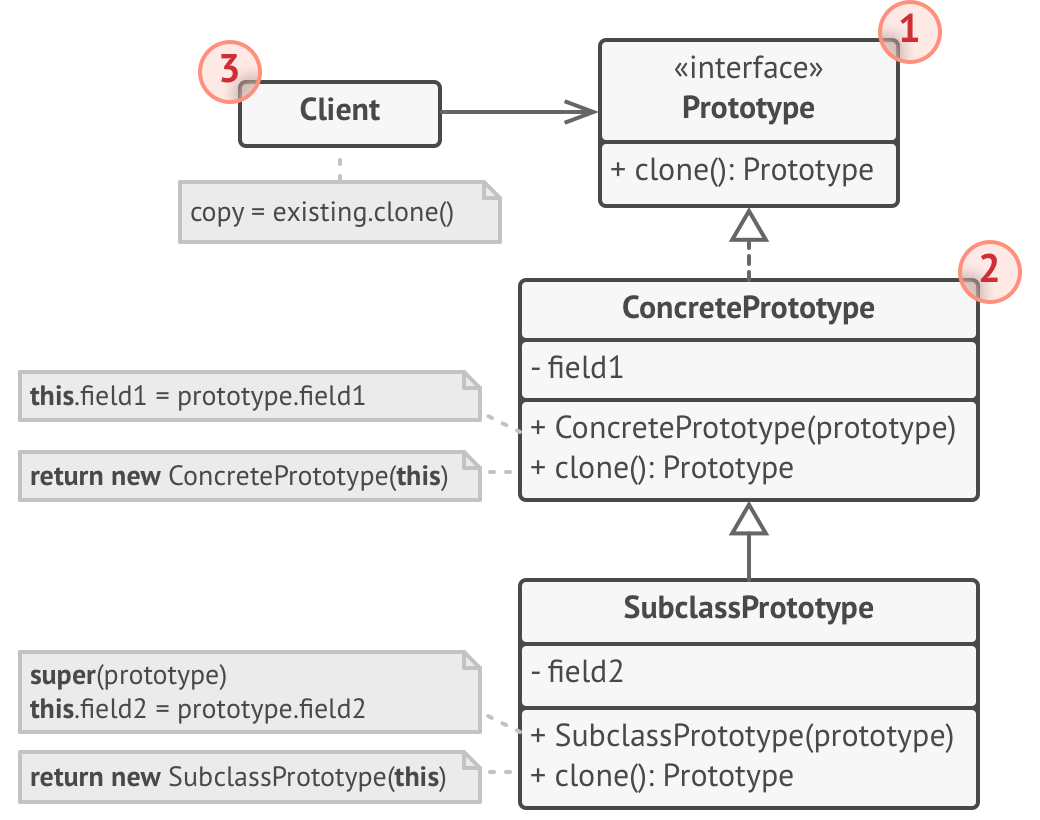
\includegraphics[width=0.7\linewidth]{res/teoria/Prototype.png}
    \caption{Struttura}
\end{figure}
\paragraph{Applicabilità}
Il pattern è applicabile quando le classi sono specificate a runtime, per evitare di costruire gerarchie di factories parallele alle gerarchie dei prodotti. Si può utilizzare quando le istanze di oggetti possono avere un numero finito di stati.

\subsubsection{Singleton}
\paragraph{Scopo}
Un \textbf{singleton} permette di assicurarsi che una classe abbia una sola istanza, fornendone un punto di accesso globale.
\paragraph{Problema}
Il singleton pattern risolve due problemi allo stesso tempo, ma \textbf{violando il Single Responsibility Principle}:
\begin{enumerate}
    \item Si assicura che una classe abbia una sola istanza: questo torna utile quando, ad esempio, lavoriamo su dati di una risorsa condivisa, sia essa un DB, un file...
    \item Fornisce un punto di accesso globale alla risorsa
\end{enumerate}
\paragraph{Soluzione}
Tutte le implementazioni del singleton hanno questi due step in comune:
\begin{itemize}
    \item Rendere il costruttore di default privato, in modo da non poter istanziare oggetti da fuori il singleton 
    \item Creare un metodo di \code{getInstance} che faccia da costruttore. Se esiste già un'istanza la restituisce, altrimenti la crea e restituisce.
\end{itemize}
\begin{figure}[H]
    \centering
    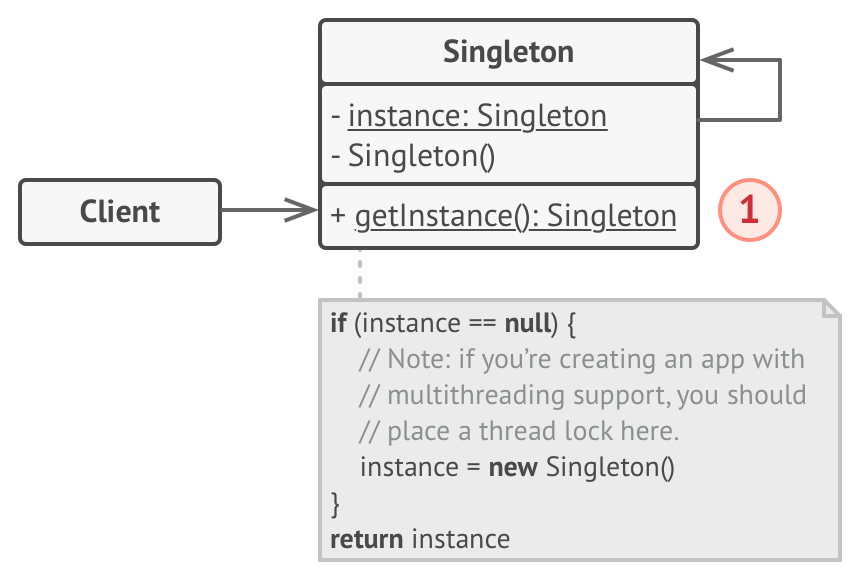
\includegraphics[width=\linewidth]{res/teoria/Singleton.png}
    \caption{Struttura}
\end{figure}
\paragraph{Applicabilità}
Lo utilizziamo quando è necessaria una sola istanza di una classe, che deve essere globalmente accessibile. 

\subsection{Structural Patterns}
\subsubsection{Adapter}
\paragraph{Scopo}
L'\textbf{adapter} permette ad oggetti con interfacce incompatibili di collaborare.

\paragraph{Problema}
Immaginiamo di star creando un'app di monitoraggio del mercato in borsa. L'app scarica i dati in XML da un'API. Ad un certo punto, vogliamo integrare un'altra API, che però restituisce dati in JSON. Potremmo cambiare questa libreria, ma sarebbe un casino. 
\paragraph{Soluzione}
Creiamo un adattatore, che converta l'interfaccia di un oggetto in un'altra, in modo da farla comprendere all'oggetto. Un adapter wrappa l'oggetto in modo da nasconderne la complessità: chi lo utilizza non è neanche al corrente del fatto che sia un adapter. 
\begin{figure}[H]
    \centering
    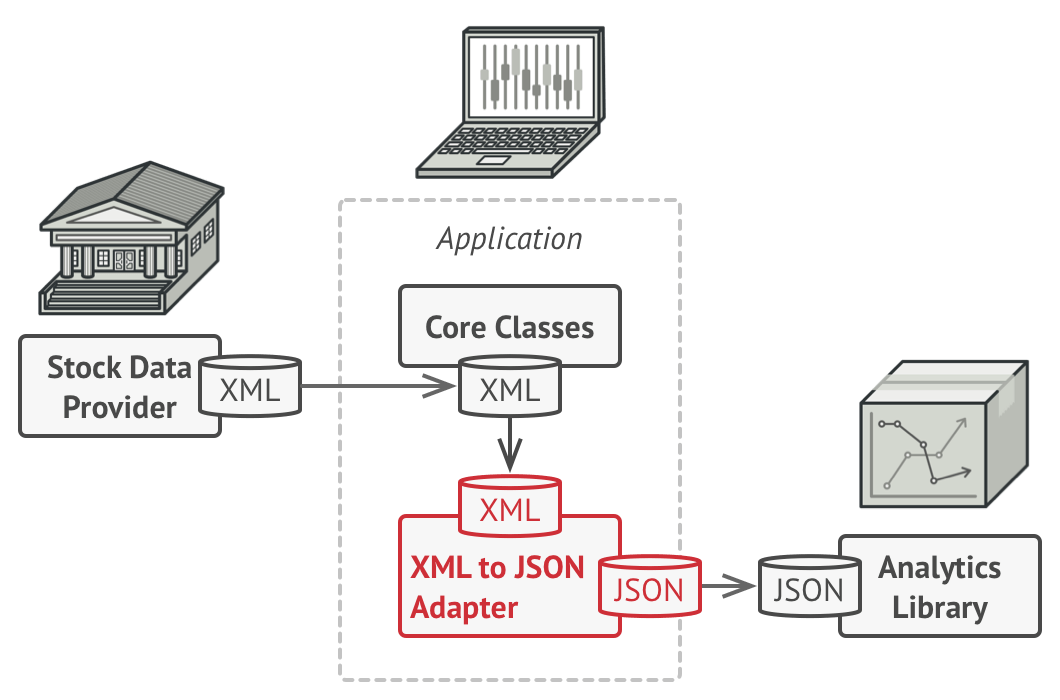
\includegraphics[width=\linewidth]{res/teoria/Adapter.png}
    \caption{Struttura}
\end{figure}
\paragraph{Applicabilità}
Lo utilizziamo quando una classe esistente fornisce la funzionalità richiesta in parte, ma non implementa l'interfaccia necessaria.

\subsubsection{Bridge}
\paragraph{Scopo}
Il \textbf{bridge} permette di splittare un grande numero di classi in due gerarchie separate, astrazione e implementazione, sviluppabili indipendentemente. 

\paragraph{Problema}
Ipotizziamo di avere una classe \code{Shape} con due subclasses: \code{Circle} e \code{Square}. Vogliamo estendere questa gerarchia per incorporare i colori, quindi inizialmente proponiamo di creare sottoclassi \code{RedCircle}, \code{BlueCircle}, \code{RedSquare}, \code{BlueSquare}. È palese che questo approccio non sia sostenibile per il futuro. 
\paragraph{Soluzione}
Semplicemente, facciamo diventare il colore una proprietà dell'oggetto \code{Shape}. In questo modo, switchamo da ereditarietà a composizione. 
\begin{figure}[H]
    \centering
    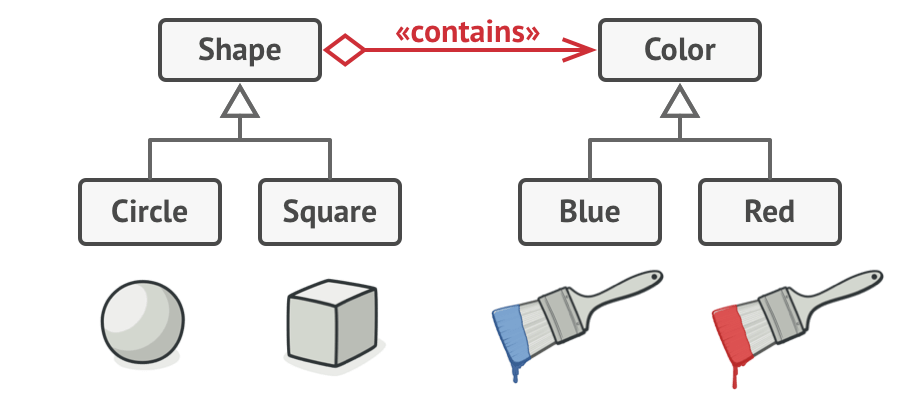
\includegraphics[width=\linewidth]{res/teoria/Bridge.png}
    \caption{Esempio}
\end{figure}
\begin{figure}[H]
    \centering
    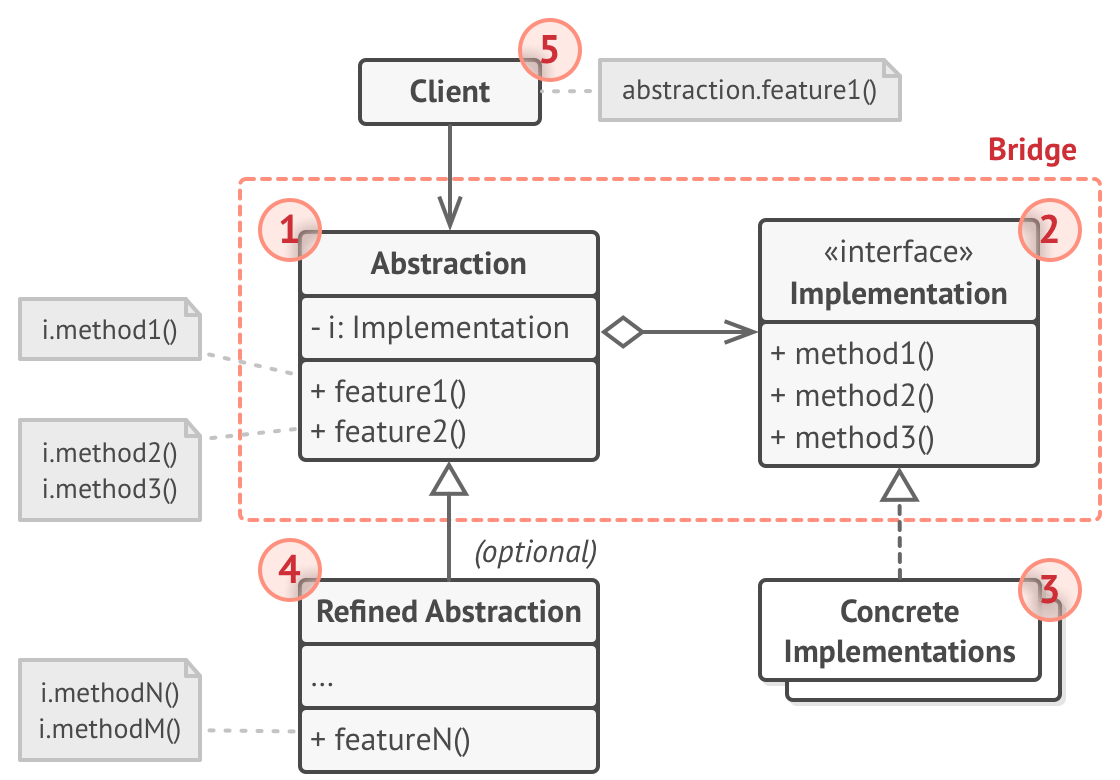
\includegraphics[width=\linewidth]{res/teoria/BridgeStructure.png}
    \caption{Struttura}
\end{figure}
\paragraph{Applicabilità}
Utilizziamo il bridge quando interfaccia ed implementazione devono variare indipendentemente. Richiede un'interfaccia comune tra gerarchie intercambiabili di classi. 
\subsubsection{Adapter vs. Bridge}
Entrambi sono utilizzati per nascondere dettagli implementativi. L'adapter fa lavorare insieme componenti incompatibili, mentre il bridge permette ad astrazioni ed implementazioni di variare indipendentemente.
\subsubsection{Composite}
\paragraph{Scopo}
Il \textbf{composite pattern} permette di comporre oggetti in strutture ad albero e lavorare su queste strutture come oggetti individuali. 

\paragraph{Problema}
Utilizzare il composite pattern ha senso solo quando il core del software è rappresentabile da un albero. Per esempio, immaginiamo di avere due tipi di oggetti: \code{Prodotto} e \code{Scatola}. Le scatole contengono, ovviamente, più oggetti, oppure altre scatole. Potremmo tentare un approccio diretto, ma sarebbe computazionalmente \textit{una merda.}
\paragraph{Soluzione}
Il composite pattern suggerisce di lavorare su prodotti e scatole attraverso un'unica interfaccia, che dichiara un metodo per calcolare il costo totale. In un prodotto, restituirebbe il costo del prodotto. In una scatola, restituisce la chiamata ricorsiva a tutti i contenuti. \textit{Avete già capito dove voglio arrivare.} In questo modo, basta chiamare il metodo di calcolo sulla scatola grande e verrà chiamato ricorsivamente su tutti i nodi. \textit{Spaventosamente elegante.}
\begin{figure}[H]
    \centering
    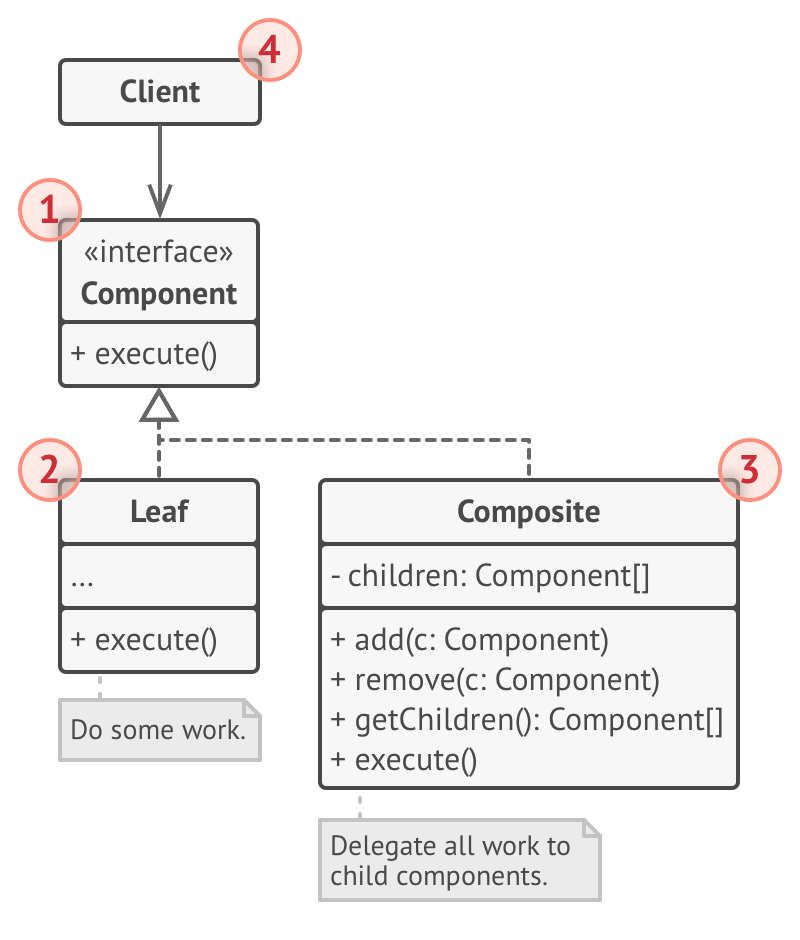
\includegraphics[width=0.6\linewidth]{res/teoria/Composite.png}
    \caption{Struttura}
\end{figure}
\paragraph{Applicabilità}
È utile quando vogliamo rimuovere responsabilità a singoli oggetti dinamicamente, ove l'estensione per subclasses non è pratica.
\subsubsection{Decorator}
\paragraph{Scopo}
Il decorator permette di \textit{agganciare} nuovi comportamenti ad oggetti, inserendoli in oggetti \textit{wrapper} che contengono questi nuovi behaviors.
\paragraph{Problema}
Immaginiamo di stare lavorando ad una libreria per notifiche, che permette ad altri software di notificare gli utenti. La versione iniziale è basata sulla classe \code{Notifier} che ha pochi field, un costruttore, ed un singolo metodo \code{send()}. Questo metodo accetta un messaggio e lo invia agli utenti specificati nel costruttore. Ad un certo punto, realizzi di voler implementare altri tipi di notifiche, come messaggi Telegram o sms. Estendi quindi la classe \code{Notifier} con delle subclasses, come \code{FacebookNotifier} o \code{SMSNotifier}. Ti chiedono, però, di poterne usare più di uno alla volta, e sarebbe da idioti cominciare a fare subclasses per ogni combinazione di notificatori.
\paragraph{Soluzione}
L'ereditarietà, in questo caso, non è la soluzione. Ci spostiamo sulla aggregazione/composizione. Il pattern Decorator è detto anche \textbf{Wrapper}. Questo esprime chiaramente l'idea di fondo: creiamo un oggetto wrapper che contiene i metodi del \textit{target} e li chiama, però svolge operazioni che alterano il risultato, prima o dopo la chiamata. Generiamo così una struttura in cui \code{Notifier} possiede un oggetto di interfaccia \code{BaseDecorator}, che ha come subclasses i vari decorator. Generiamo così uno stack, che passiamo alla generazione di un nuovo decorator. Esso, tramite \code{super}, chiama i vari decorator della stack \textit{in salita.} L'unico decorator che effettivamente viene chiamato è sempre l'ultimo. 
\begin{figure}[H]
    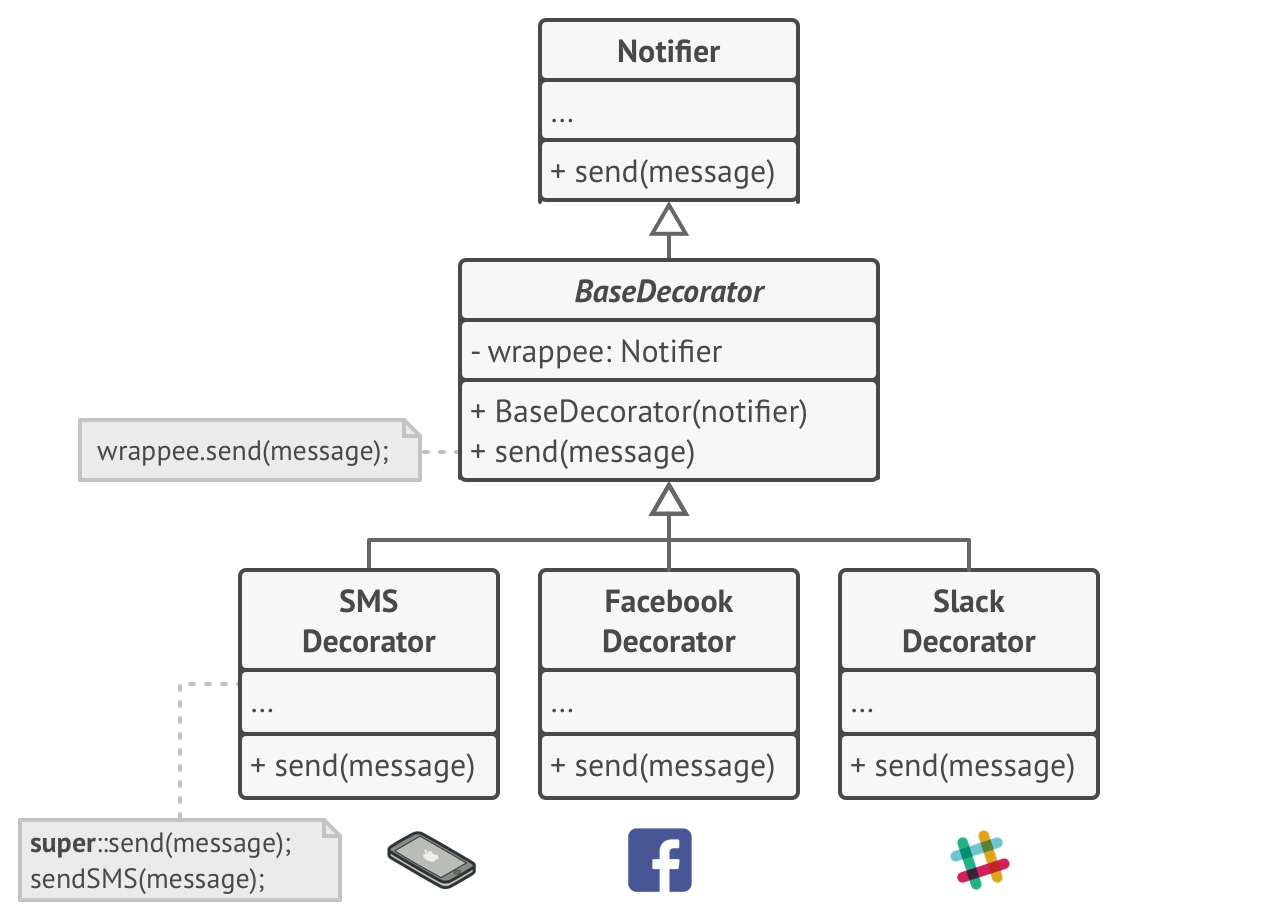
\includegraphics[width=0.5\linewidth]{res/teoria/Decorator1.png}
    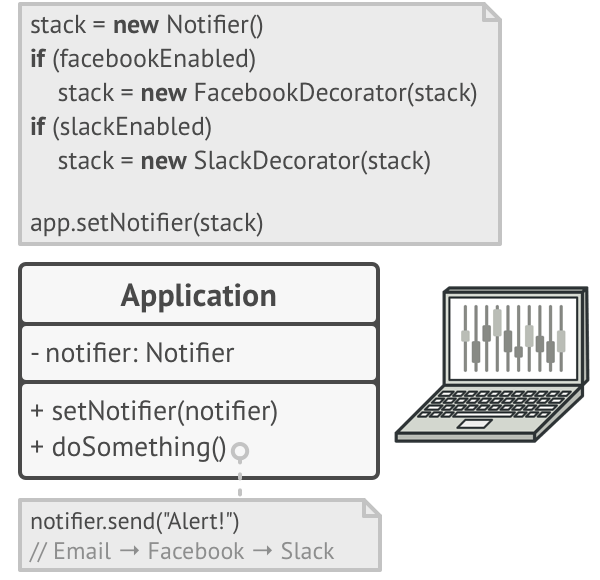
\includegraphics[width=0.5\linewidth]{res/teoria/Decorator2.png}
    \caption{Struttura}
\end{figure}
\paragraph{Applicabilità}
Lo utilizziamo quando è utile aggiungere/rimuovere comportamenti agli oggetti \textbf{dinamicamente}, e l'estensione per subclasses non è conveniente.

\subsubsection{Facade}
\paragraph{Scopo}
Una \textbf{facade} è un pattern che fornisce un'interfaccia semplificata ad una libreria, un framework, o qualsiasi altro set complesso di classi.
\paragraph{Problema}
Immaginiamo di dover far funzionare il nostro codice con un set molto grande di oggetti che appartengono ad un sofisticato framework. Dovremmo, prima di tutto, inizializzare tutti gli oggetti, tenere traccia delle dipendenze, eseguire metodi nell'ordine corretto, e via dicendo. Il funzionamento del software diventerebbe quindi molto dipendente da questo framework.
\paragraph{Soluzione}
Una facade è una classe che fornisce una semplice interfaccia a un sottosistema complesso che contiene molti componenti. Essa fornisce funzionalità limitate, ma sufficienti all'utilizzo specifico che serve. 
\paragraph{Applicabilità}
La utilizziamo per fornire un'interfaccia semplice a un sottosistema complesso, e \textit{decouplare} le classi del subsystem dal nostro software.
\paragraph{Struttura ideale di un subsystem}
Un buon subsystem è basato su:
\begin{itemize}
    \item Un'interfaccia
    \item Oggetti di controllo
    \item Oggetti di entità
\end{itemize}
E fa utilizzo di design pattern, come Adapter e Bridge.

\subsubsection{Flyweight}
\paragraph{Scopo}
Il \textbf{flyweight} permette di ridurre lo spazio di memoria necessario al salvataggio di oggetti, salvando le parti in comune.  
\paragraph{Problema}
Immaginiamo di dover creare un videogioco sparatutto. Decidiamo di implementare un sistema di particelle complesso, in modo che proiettili, missili, detriti siano gestiti da oggetti. Avremmo quindi una struttura in cui ogni particella occupa molto spazio in memoria:
\begin{figure}[H]
    \centering
    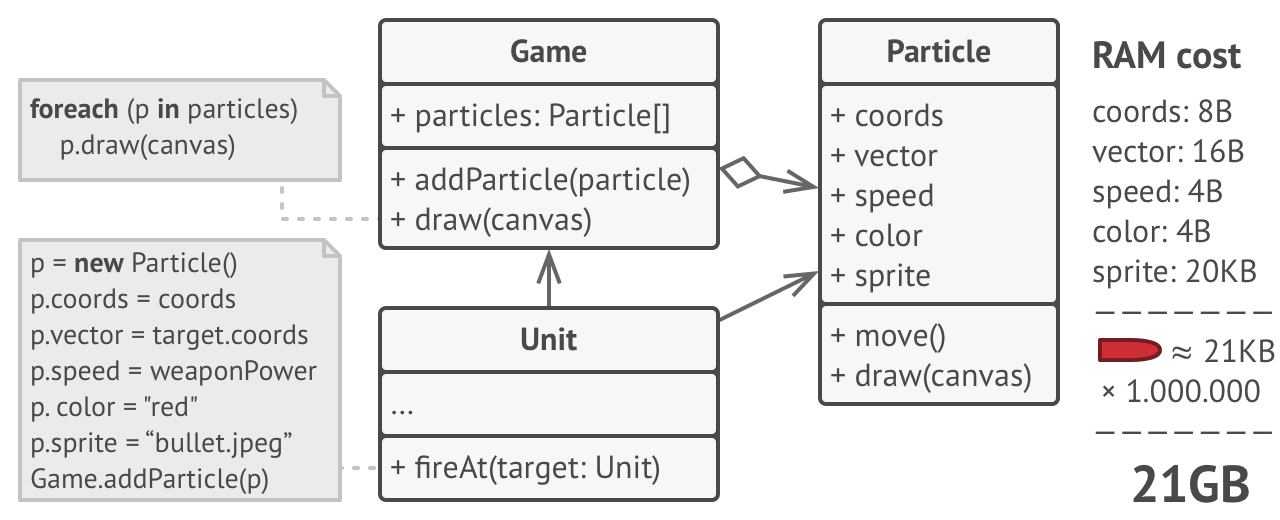
\includegraphics[width=\linewidth]{res/teoria/FlyweightProblem.png}
    \caption{Struttura iniziale}
\end{figure}
\paragraph{Soluzione}
Notiamo però che molte informazioni sono ripetute! Infatti, ad esempio, colore e sprite, che occupano moltissima memoria, contengono quasi sempre gli stessi dati. Decidiamo, allora, di salvare le informazioni comuni in una classe a parte, in modo da salvare solo il minimo indispensabile per le singole particelle. 
\begin{figure}[H]
    \centering
    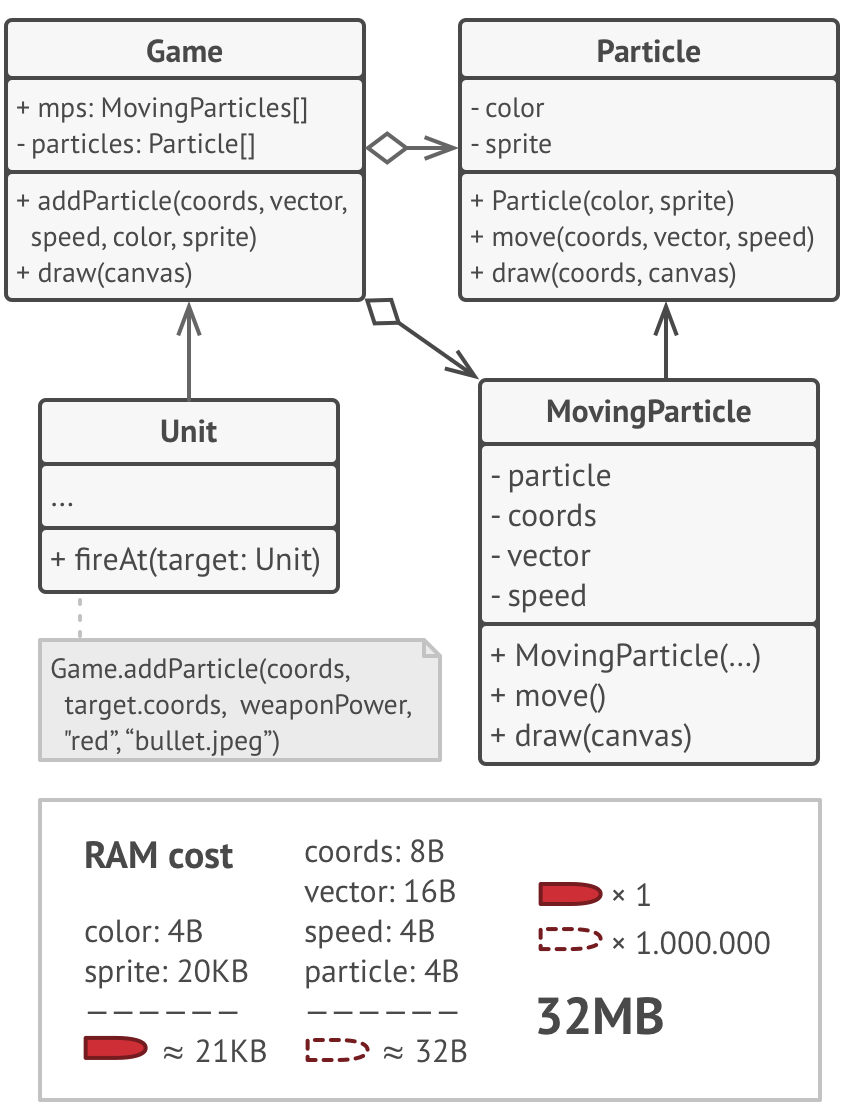
\includegraphics[width=0.6\linewidth]{res/teoria/FlyweightSolution.png}
    \caption{La soluzione usando il Flyweight pattern}
\end{figure}
\paragraph{Applicabilità}
Utilizziamo questo pattern quando abbiamo un \textbf{grande numero di oggetti}, con costi in memoria alti, stati che possono essere estratti dall'oggetto, ed un'applicazione che non dipende dall'identità degli oggetti. 
\subsubsection{Proxy}
\paragraph{Scopo}
Il \textbf{proxy} permette di avere un sostituto ad un oggetto, controllandone l'accesso da parte degli altri, e potendo eseguire operazioni prima e dopo. 
\paragraph{Problema}
Perché dovremmo controllare l'accesso? Per esempio, se avessimo un oggetto che usa molte risorse di sistema ma che non utilizziamo sempre, sarebbe utile avere un \textit{lazy loading}, ossia un'istanziazione solo quando necessario. 

\paragraph{Soluzione}
Creiamo quindi una classe proxy che abbia la stessa interfaccia dell'oggetto desiderato. In questo modo, agli oggetti che lo richiedono, lo passiamo al posto dell'oggetto vero e proprio. Il proxy crea quindi l'oggetto vero solo dopo la prima richiesta. Se, inoltre, volessimo filtrare i risultati ottenuti, potremmo farlo, un po' come accade in un Decorator.
\begin{figure}[H]
    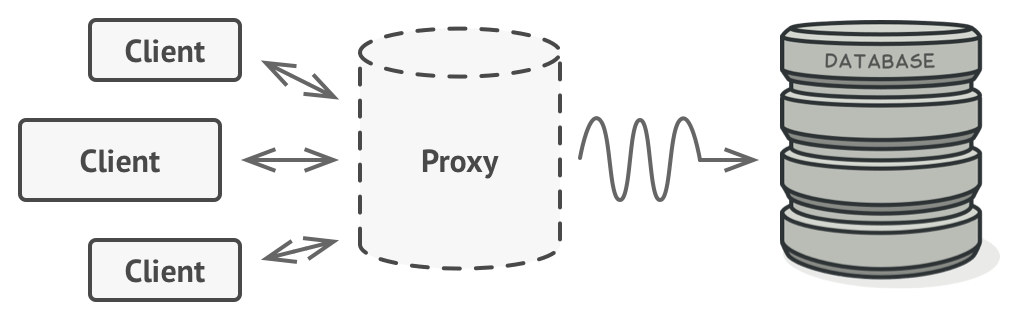
\includegraphics[width=\linewidth]{res/teoria/Proxy.png}
    \caption{La soluzione usando il Flyweight pattern}
\end{figure}
\paragraph{Applicabilità}
Lo utilizziamo quando abbiamo necessità di \textbf{controllare l'accesso} ad un oggetto, e necessitiamo di una reference sofisticata al suddetto.
\paragraph{Tipologie}
Abbiamo più tipologie di proxy:
\begin{itemize}
    \item Virtual proxy (expensive objects) 
    \item Cache proxy (temporary objects) 
    \item Remote proxy (remote objects)
    \item Protection proxy (shared objects)
    \item Smart reference (pointer extension)
\end{itemize}
\subsection{Behavioral patterns}
A volte è necessario eseguire richieste agli oggetti senza conoscenze sull'operazione richiesta o il destinatario della stessa. Un esempio possono essere le librerie grafiche per bottoni e menù, che non implementano l'azione ma passano la richiesta. I behavioral patterns si occupano di questo: gestiscono l'assegnamento di responsabilità tra oggetti.
\subsubsection{Chain of responsibility}
\paragraph{Scopo}
La \textbf{chain of responsibility} permette di passare richieste attraverso una catena di \textit{handlers}. Quando riceve una richiesta, ogni handler decide se processarla o passarla al prossimo handler della catena.
\paragraph{Problema}
Immaginiamo di lavorare a un sistema di ordini online. Vogliamo restringere l'accesso al sistema, in modo che solo gli utenti autenticati possano ordinare. Vogliamo inoltre degli amministratori, che possano vedere tutti gli ordini. Decidiamo che questi controlli devono essere fatti in sequenza: se l'autenticazione fallisce, non è necessario fare altre verifiche. Col tempo, si aggiungono altre verifiche: un sanitizing dei dati, una verifica degli IP, un motore di caching. Ad ogni verifica aggiunta, il codice diventa un porcilaio.
\paragraph{Soluzione}
Trasformiamo quindi queste verifiche in \textit{handlers}: ognuna avrà un metodo \code{check}, ed un campo per il prossimo handler della catena. Ad ogni richiesta, l'handler eseguirà le sue verifiche: se è tutto ok, passerà la richiesta al prossimo handler, altrimenti fermerà il tutto. È fondamentale che tutti gli handler implementino una stessa interfaccia. 
\begin{figure}[H]
    \centering
    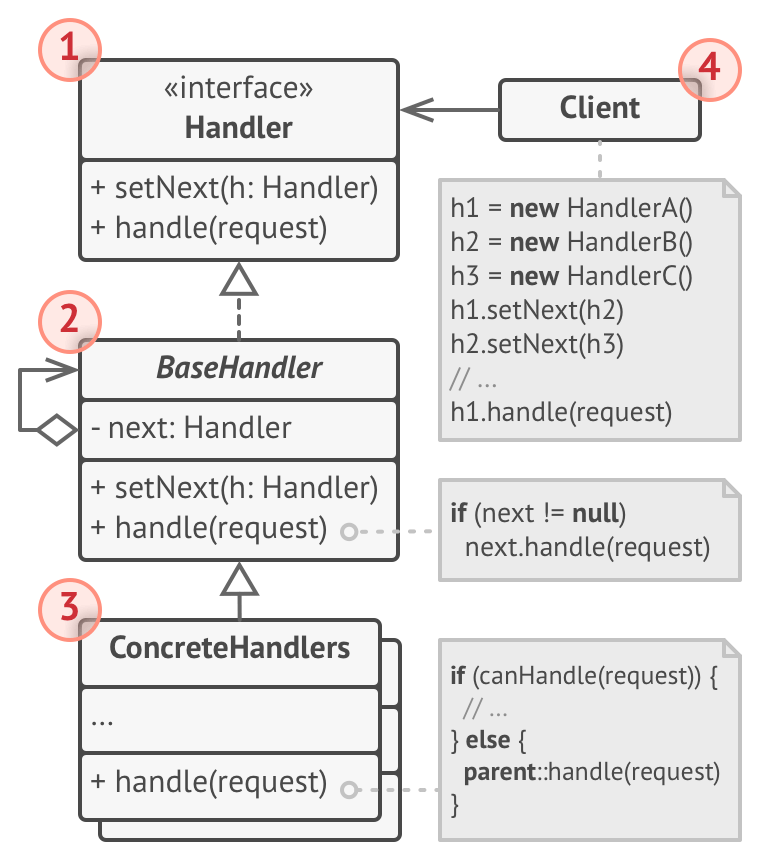
\includegraphics[width=0.6\linewidth]{res/teoria/Handler.png}
    \caption{La soluzione}
\end{figure}
\paragraph{Applicabilità}
Utilizziamo questo pattern quando più di un oggetto deve eseguire un comando, l'handler non è conosciuto in anticipo e non può ssere determinato automaticamente.
\subsubsection{Command}
\paragraph{Scopo}
Il \textbf{command} trasforma una richiesta in un oggetto \textit{stand-alone} che contiene tutte le informazioni che la riguardano. Questo pattern può essere utilizzato per \textit{decouplare} i boundary e control objects.
\paragraph{Problema}
Immaginiamo di lavorare ad un software di text editing. Vogliamo creare una toolbar che contenga tasti per le operazioni più importanti, con una classe \code{Button}. Cominciamo a creare subclasses per ogni bottone necessario: \code{OKButton}, \code{SaveButton}, \code{ApplyButton}, ed ogni tasto che si aggiunge, \textit{la nostra voglia di vivere cala.} Dev'esserci un modo più furbo.
\paragraph{Soluzione}
Estraiamo i dati della richiesta tramite un oggetto dall'interfaccia \code{Command}, che avrà come implementazioni i vari tipi di comando possibili, aventi un solo metodo \code{execute}. In questo modo, ogni bottone chiamerà l'\code{execute} del suo \code{Command}, ma non solo: i comandi potrebbero, ad esempio, anche essere chiamati da scorciatoie da tastiera!
\begin{figure}[H]
    \centering
    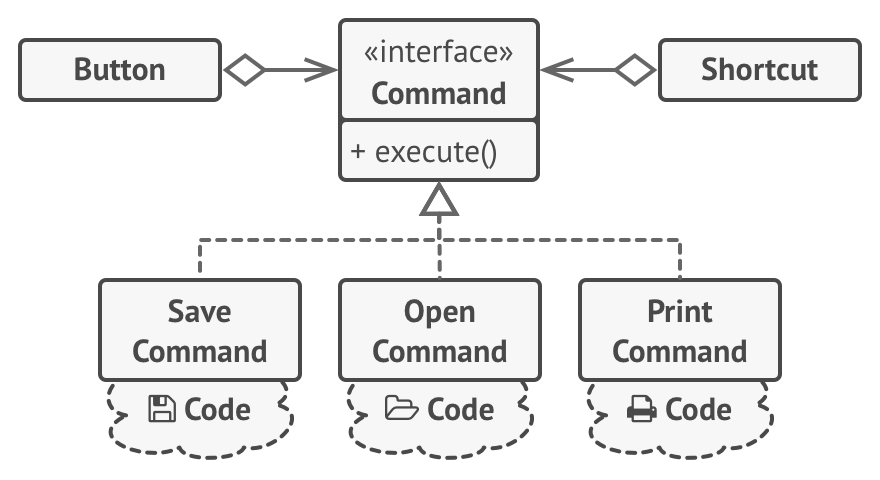
\includegraphics[width=0.6\linewidth]{res/teoria/Command.png}
    \caption{Soluzione usando un Command}
\end{figure}
\paragraph{Applicabilità}
Lo utilizziamo per parametrizzare oggetti con un'azione da eseguire, specificando le queue di azioni ed eseguire richieste in tempi diversi. Supportiamo così l'undo/redo.
\subsubsection{Interpreter}
\paragraph{Scopo}
L'\textbf{interpreter}, dato un linguaggio, definisce una rappresentazione per la sua grammatica ed un modo di interpretarne le frasi. Mappa un dominio ad un linguaggio, il linguaggio ad una grammatica, e la grammatica ad un design object-oriented gerarchico.
\paragraph{Problema}
Abbiamo una classe di problemi appartenenti ad un dominio ben definito. Se il dominio è caratterizzato da un linguaggio, il problema può essere risolto tramite un interprete. 
\paragraph{Soluzione}
Modelliamo il dominio con una grammatica ricorsiva ad albero, in cui ogni regola è un nodo o una foglia. 
\begin{figure}[H]
    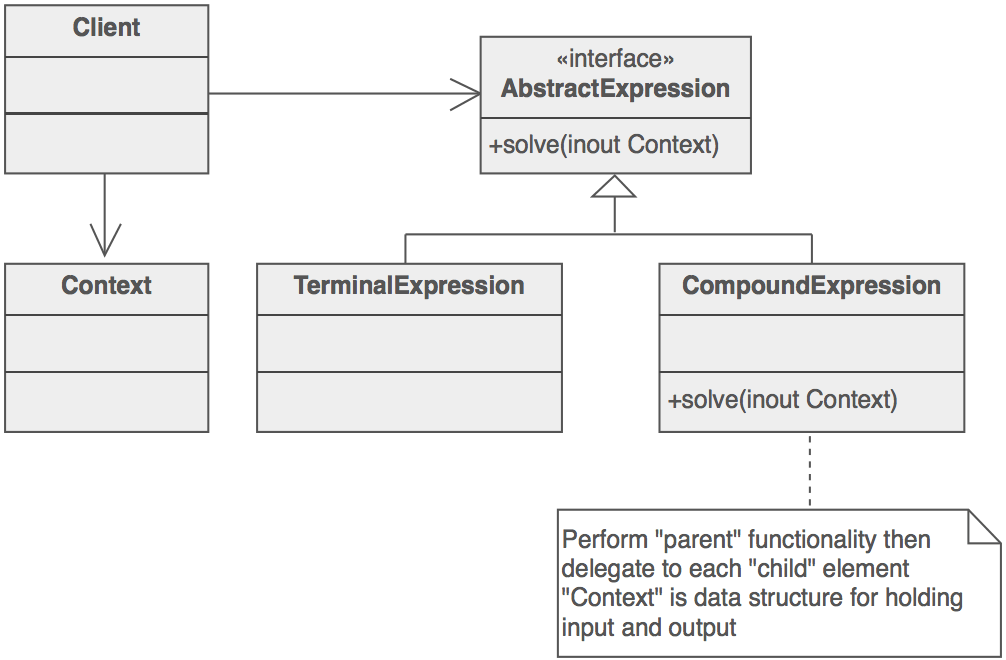
\includegraphics[width=\linewidth]{res/teoria/Interpreter.png}
    \caption{Struttura di un interpreter}
\end{figure}
\paragraph{Applicabilità}
Utilizzabile quando abbiamo un linguaggio facilmente mappabile con un albero, con grammatica semplice ed efficienza non importante.
\subsubsection{Iterator}
\paragraph{Scopo}
L'\textbf{iterator} permette di attraversare gli elementi di una collection senza esporne le logiche di rappresentazione.
\paragraph{Problema}
Creiamo un nostro oggetto di collection per salvare dati, con una struttura \textit{cazzutissima} ed ultra segreta, che ci permetterà di diventare milionari grazie all'intelligentissimo metodo di esplorazione dei dati che ho. Abbiamo ora un problema: non vogliamo esporre le logiche con cui esploriamo la collection. 
\paragraph{Soluzione}
Estraiamo l'esplorazione della collection tramite un oggetto \textit{iterator}. Potremmo addirittura avere più iterators, che implementino un'interfaccia costituita da: un metodo \code{getNext}, un metodo \code{hasNext}, ed un campo che salvi l'elemento corrente. 
\begin{figure}[H]
    \centering
    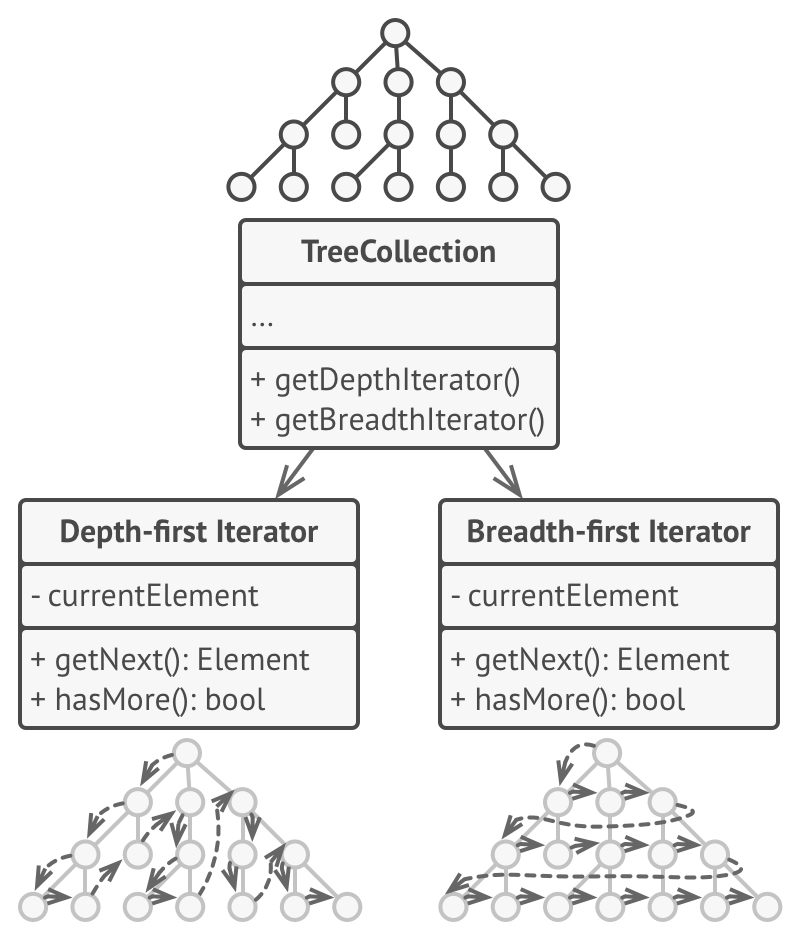
\includegraphics[width=0.6\linewidth]{res/teoria/Iterator.png}
    \caption{Struttura di un iterator multiplo}
\end{figure}
\paragraph{Applicabilità}
Lo utilizziamo per accedere ad una collection senza esporne l'implementazione, supportando esplorazioni simultanee, e fornendo un'unica interfaccia per l'esplorazione di collections diverse.
\subsubsection{Mediator}
\paragraph{Scopo}
Il \textbf{mediator} permette di ridurre le caotiche dipendenze tra oggetti. Esso restringe la comunciazione diretta tra gli oggetti e li forza a collaborare solo tramite un oggetto mediator. 

\paragraph{Problema}
Immaginiamo di avere un dialogo di creazione e modifica dei profili utente, composto da textfields, checkboxes, bottoni. Alcuni di questi elementi devono collaborare: ad esempio, selezionando la checkbox "Sono Guido Soncini", il titolo diventerà "Reggio Merda". Applicare questa logica all'interno degli elementi è un bagno di sangue.
\paragraph{Soluzione}
Creiamo quindi un oggetto \code{Mediator} che regoli la comunicazione tra questi oggetti, chiamato dai suddetti a necessità. Nel nostro esempio, la classe \code{Dialog} potrebbe fungere da mediator. A questo punto, cambiamo la logica degli elementi: essi non avranno più verifiche e implementazioni al loro interno, ma semplicemente notificheranno \code{Dialog} delle loro modifiche di stato. 
\begin{figure}[H]
    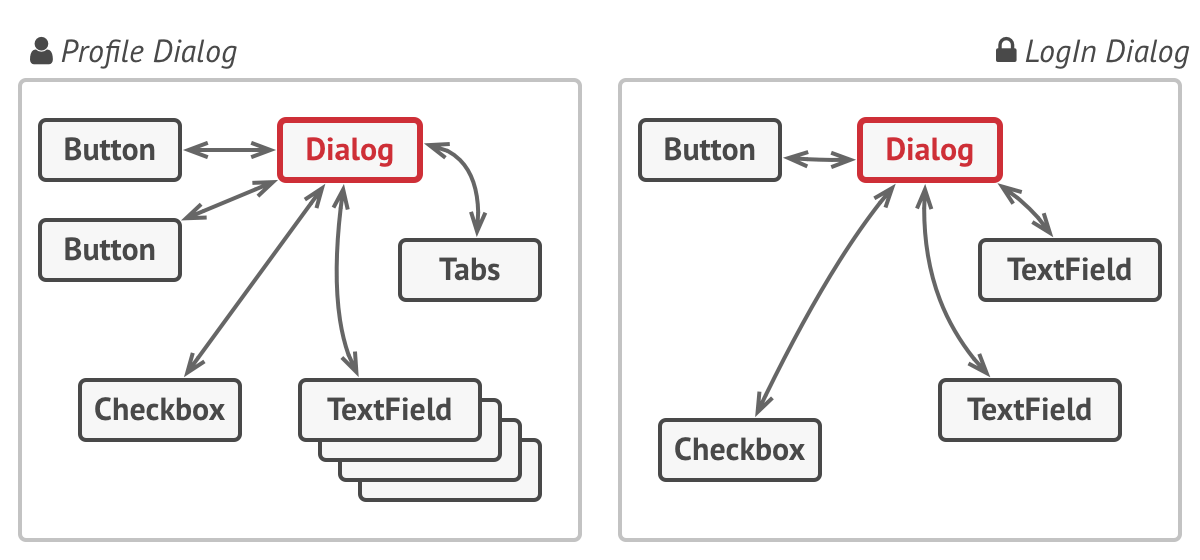
\includegraphics[width=\linewidth]{res/teoria/Mediator.png}
    \caption{Struttura del dialog}
\end{figure}
\paragraph{Applicabilità}
Lo utilizziamo quando un set di oggetti deve comunicare in modo definito ma complesso, ed il riutilizzo degli oggetti è complesso perché sono pieni di logica. Un behavior distribuito tra diverse classi dovrebbe essere customizzabile senza troppo subclassing. 

\subsubsection{Memento}
\paragraph{Scopo}
Il \textbf{Memento} permette di salvare e ripristinare lo stato di oggetti senza rivelarne i dettagli implementativi. 
\paragraph{Problema}
Immaginiamo di creare un software di text editing. Sarebbe molto comodo avere un tasto undo per annullare le operazioni. Per salvare però lo stato dell'editor, dovremmo salvare tutti i suoi fields. Il problema risulta ovvio: non possiamo accedere a field privati dall'esterno. 
\paragraph{Soluzione}
Creiamo allora una classe \code{Snapshot}, che contenga i dati necessari al salvataggio, ed abbia oggetti generati dal protagonista del salvataggio, che avrà un metodo \code{makeSnapshot} ed un metodo \code{restore}. In questo modo, potremmo decidere di lasciare pubbliche alcuni metadata dello snapshot, come la data o l'utente, senza pubblicarne il contenuto. Possiamo ora salvare gli snapshot all'interno di oggetti detti \textit{caretakers}. 
\paragraph{Applicabilità}
Utilizziamo il pattern quando vogliamo salvare lo stato di un oggetto per ripristinarlo, senza però rendere pubblici dati privati. 

\subsubsection{Observer}
\paragraph{Scopo}
L'\textbf{observer} è un pattern che permette di defininire un meccanisco di \textit{iscrizione} per notificare più oggetti di eventi che accadono.
\paragraph{Problema}
Immaginiamo due tipi di oggetto, \code{Customer} e \code{Store}. Il customer è interessato all'uscita di un nuovo modello di telefono: potrebbe visitare il negozio tutti i giorni per verificarne la disponibilità, ma questo, in termini prestazionali, fa cagare.
Il negozio potrebbe, invece, inviare avvisi a tutti i clienti, anche quelli non interessati, ma questo farebbe arrrabbiare i clienti.
\paragraph{Soluzione}
Il pattern Observer suggerisce di aggiungere un meccanismo di subscription in modo da poter iscrivere determinati clienti alle notifiche. In questo modo, il publisher avrà una lista di subscribers, aventi un metodo \code{update()} utile alla notifica di eventi. 
\begin{figure}[H]
    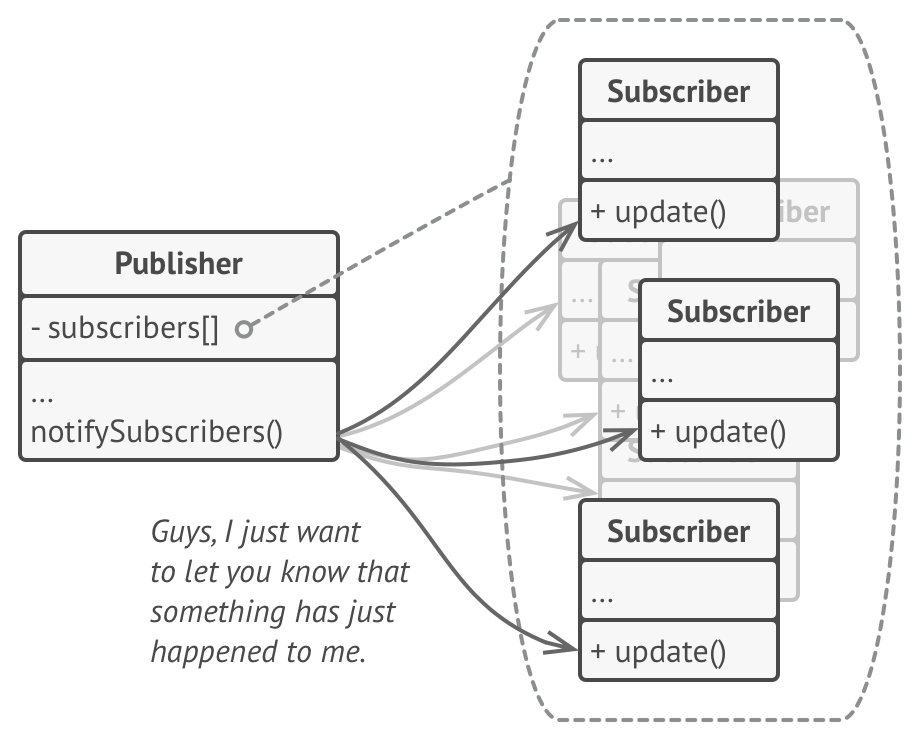
\includegraphics[width=\linewidth]{res/teoria/Observer.png}
    \caption{Struttura}
\end{figure}
\paragraph{Applicabilità}
Lo utilizziamo quando un'astrazione ha due aspetti, uno dipendente dall'altro, ed un cambiamento ad uno degli oggetti richiede cambiamenti all'altro. 

\subsubsection{State}
\textit{Questo non è nelle slide.}
\paragraph{Scopo}
Lo \textbf{State} permette ad un oggetto di alterare il suo comportamento alla modifica del suo stato. All'apparenza, l'oggetto sembra aver cambiato classe.
\paragraph{Problema}
Lo state pattern è molto legato al concetto di macchina a stati finiti. L'idea di fondo è che in ogni momento esiste un numero \textbf{finito} di stati possibili per il programma. Immaginiamo di avere una classe \code{Document}, avente tre stati: \code{Draft}, \code{Moderation} e \code{Published}. Solitamente vengono utilizzati degli \code{switch..case} per modificare il comportamento in base alla proprietà \code{state}.
\paragraph{Soluzione}
L'alternativa è creare un interfaccia \code{State} implementata da tutti i possibili stati dell'oggetto, e dare all'oggetto una proprietà \code{state}. In questo modo, lo state potrà contenere i metodi variabili.  
\begin{figure}[H]
    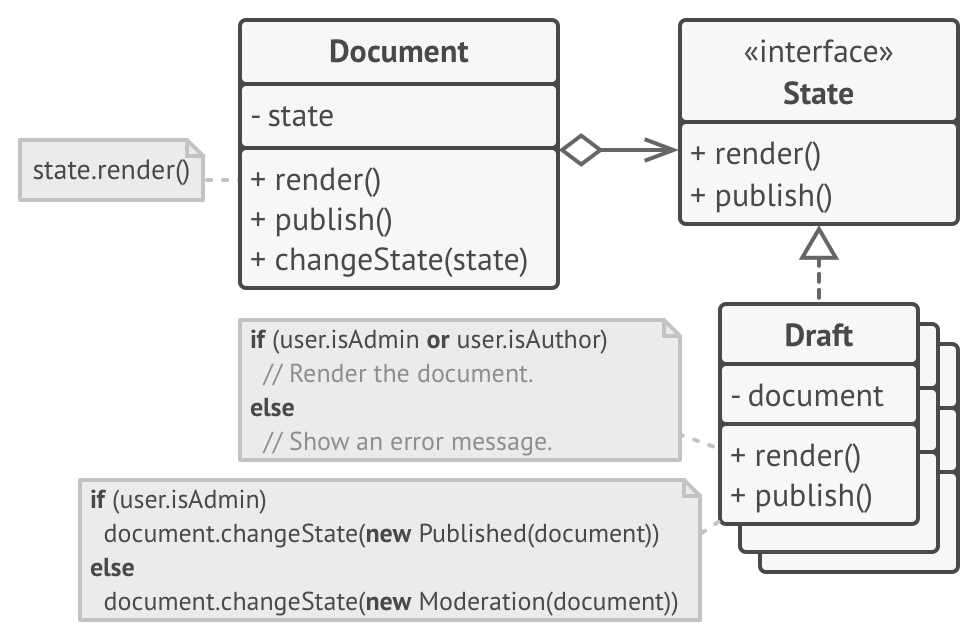
\includegraphics[width=\linewidth]{res/teoria/State.png}
    \caption{Struttura}
\end{figure}
\subsubsection{Strategy}
\paragraph{Scopo}
Lo \textbf{strategy} è un pattern che permette di definire una famiglia di algoritmi, inserirli in classi separate, e renderne gli oggetti intercambiabili. 
\paragraph{Problema}
Stiamo creando un'app di navigazione per viaggiatori. Vogliamo implementare una funzione di calcolo itinerari, in cui l'utente possa trovare l'itinerario più veloce da un punto A ad un punto B. In una prima versione, implementiamo solo il calcolo per auto. Gli amanti della bicicletta, però, si incazzano. Cominciamo ad implementare vari metodi di calcolo di percorsi, ma a breve la nostra classe \code{Navigator} diventa uno schifo. 
\paragraph{Soluzione}
Lo strategy pattern suggerisce di estrarre i vari modi di eseguire un'operazione in una classe separata. In questo modo, il \textbf{context}, ossia la classe originale, avrà un campo che salvi uno di questi oggetti. Nel nostro esempio di prima creeremmo un'interfaccia \code{RouteStrategy}, implementata, ad esempio, da \code{RoadStrategy}, \code{BikeStrategy} ed implementante un metodo \code{BuildRoute}. 
\begin{figure}[H]
    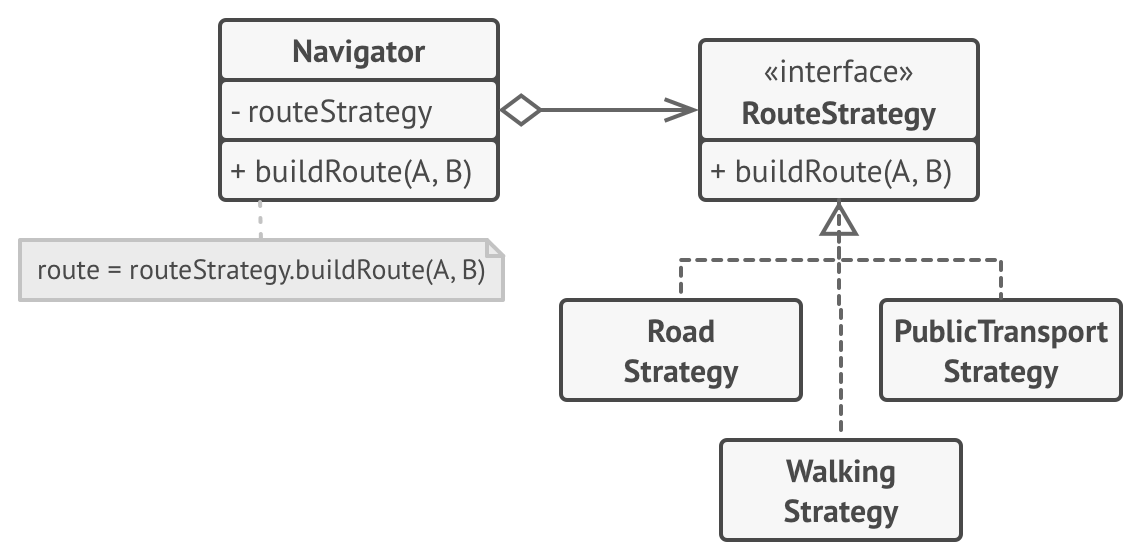
\includegraphics[width=\linewidth]{res/teoria/Strategy.png}
    \caption{Struttura}
\end{figure}
\paragraph{Applicabilità}
Lo utilizziamo quando un oggetto può essere configurato per utilizzare algoritmi multipli incapsulabili e ricopribili da una sola interfaccia.

\subsubsection{Template}
\paragraph{Scopo}
Il \textbf{template} è un pattern che permette di definire lo scheletro di un algoritmo nella sua superclasse, ma permette alle subclasses di overridare passaggi specifici dell'algoritmo senza modificarne la struttura.  
\paragraph{Problema}
Stiamo creando un'app di data mining che analizza documenti di vario tipo: DOC, CSV, PDF. Ad un certo punto notiamo che queste classi hanno molto codice in comune. 
\paragraph{Soluzione}
Il template pattern suggerisce di dividere un metodo in più step, in modo da poter overridare solo il necessario. Gli steps potrebbero essere implementati o abstract. 
\begin{figure}[H]
    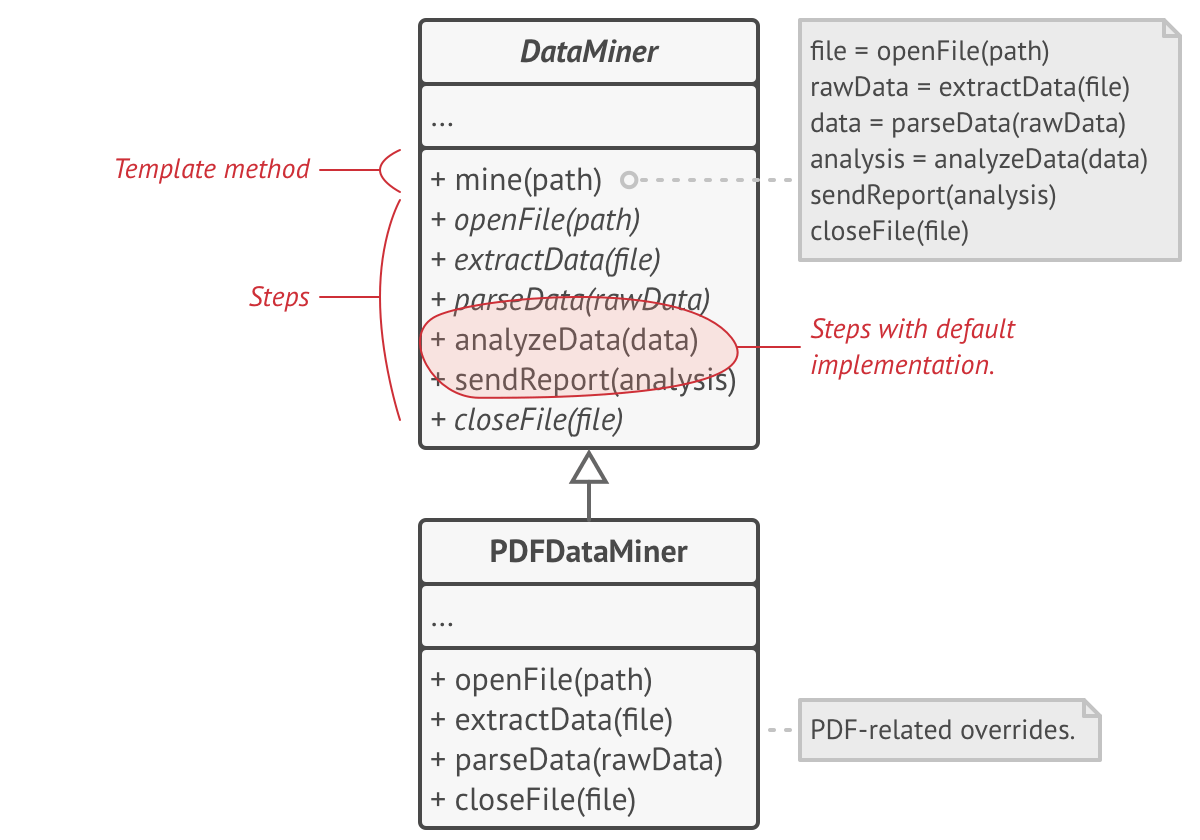
\includegraphics[width=\linewidth]{res/teoria/Template.png}
    \caption{Struttura}
\end{figure}
\paragraph{Applicabilità}
Lo utilizziamo per implementare aspetti invarianti di un algoritmo quando le subclasses ne definiscono solo alcuni passaggi. In questo modo aumentiamo il riutilizzo del codice, e controlliamo le estensioni di subclass.

\subsubsection{Visitor}
\paragraph{Scopo}
Il \textbf{visitor} permette di separare gli algoritmi dagli oggetti su cui operano. 
\paragraph{Problema}
Immaginiamo di dover creare un'app che funziona con informazioni geografiche strutturate in un grande grafo. Ogni nodo può essere rappresentato da un'entità complessa, o atomica. I nodi sono connessi ad altri da strade. Vogliamo però esportare il grafo in XML, fattibile, ad esempio, aggiungendo un metodo \code{export} ai nodi. Il PM non vuole però farci modificare il codice dei nodi. 
\paragraph{Soluzione}
Il pattern \textbf{visitor} suggerisce di inserire il nuovo comportamento in una classe detta \textit{visitor}, che abbia più metodi per ogni classe dei tipi possibili. Questo però crea un problema: come fare a scegliere il metodo giusto? Implementiamo nei nodi un metodo \code{accept}, che prende in input il visitor e ne chiama il metodo adatto. Abbiamo sì modificato la classe nodo, ma in un modo poco distruttivo. 
\begin{figure}[H]
    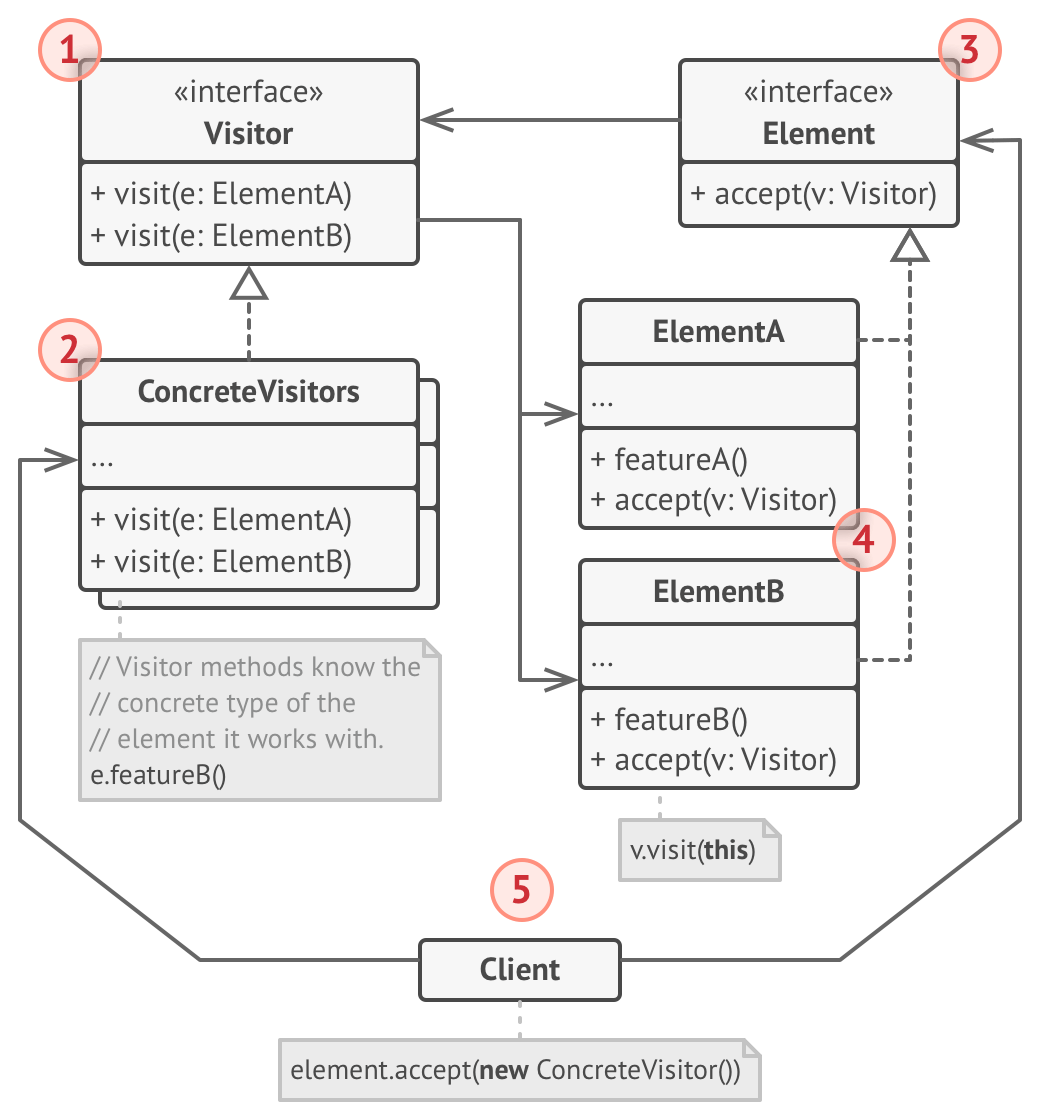
\includegraphics[width=\linewidth]{res/teoria/Visitor.png}
    \caption{Struttura}
\end{figure}
\paragraph{Applicabilità}
Lo utilizziamo quando operazioni simili devono essere eseguite su un gruppo di oggetti di diversi tipi, ma salvati nella stessa struttura. La struttura degli oggetti è difficilmente modificata, ma è probabile avere nuove operazioni. 
\section{T17 - Architectural design}
Il \textbf{design architetturale} permette di comprendere l'organizzazione ed il design della struttura generale di un sistema software. È il collegamento tra design e requirements engineering. Identifica i componenti strutturali e le loro relazioni in un processo creativo, quindi differente da sistema a sistema, ottenendo uno o più \textbf{modelli architetturali}. L'architettura è un modello di alto livello che descrive gli aspetti critici del sistema ed è comprensibile alla maggior parte degli stakeholders, permettendo la valutazione delle proprietà di sistema prima della sua esistenza. fornisce strumenti e tecniche per costruire il sistema. 
\subsection{Software architecture}
I risultati principali della \textbf{software architecture} sono gli aspetti rilevanti dell'architettura, una rappresentazione comprensibile, l'implementazione di strumenti e tecniche. Essa è una traccia che identifica componenti, interazioni, interconnessioni ed è definita in modo formale o informale. È fondamentale avere un vocabolario condiviso e ricco. 
\subsection{Elementi architetturali}
Un subsystem è un sistema unico, le quali operazioni sono indipendenti dai servizi di altri subsystems. Un modulo è un componente di sistema che fornisce servizi ad altri componenti, ma non può essere considerato un subsystem.
\paragraph{Componenti} Essi sono unità di computazione o data stores: clients, servers, databases, filtri, layers. Possono essere semplici o composti(subsystem). Un architettura consistente in più componenti compositi è un sistema di sistemi. 
\paragraph{Connettori} Sono elementi architetturali che modellano le interazioni tra componenti e le regole che le governano. Le interazioni si dividono in semplici (chiamate procedurali, variabili condivise) e complesse/semantically rich (client-server, database access, async, piped data streams)
\paragraph{Configurazioni} Sono grafi connessi di componenti e connettori che descrivono strutture architetturali identificanti connettività, proprietà concorrenti/distribuite, aderenza ad euristiche/stili. I componenti compositi sono configurazioni.
\subsection{Architectural design process}
Tre fasi:
\begin{itemize}
    \item \textbf{System structuring}: il sistema è decomposto in sottosistemi, e viene identificata la comunicazione tra sottosistemi
    \item \textbf{Control modeling}: stabilire un modello delle relazioni di controllo tra le parti 
    \item \textbf{Modular decomposition}: i subsystem identificati sono decomposti in moduli 
\end{itemize}
\subsubsection{Box and line diagrams}
Sono diagrammi semplici ed informali che mostrano i subsystem e le loro relazioni. Mancano di semantica, non mostrando i tipi di relazioni o le proprietà. I requisiti per la semantica dei modelli dipendono da come il modello è usato. 
\subsubsection{Software architecture views}
\begin{itemize}
    \item \textbf{Logical view}: mostra le astrazioni chiave del sistema come oggetti o classi (class/state diagrams)
    \item \textbf{Process view}: mostra come i processi interagiscono a runtime, quindi gli aspetti dinamici e le attività, la concorrenza e sincronizzazione. Usa activity, sequence e communication diagrams.
    \item \textbf{Development view}: mostra come il software verrà decomposto per lo sviluppo, dalla prospettiva del programmatore. Utilizza component e package diagrams.
    \item \textbf{Physical view}: mostra l'hardware di sistema e come il software è distribuito tra processori/nodi. Utilizza deployment diagrams.
\end{itemize}
Gli step per questo design sono \textbf{capire i requirements}, \textbf{definire l'architettura}, \textbf{rappresentare e comunicare l'architettura}, \textbf{valutare l'architettura}. Si utilizzano implementazione, miglioramento e manutenzione. 
\subsubsection{Non functional requirements}
\begin{itemize}
    \item \textbf{Performance}: localizzare operazioni critiche e minimizzare la comunicazione 
    \item \textbf{Security}: utilizzare un'architettura a strati 
    \item \textbf{Safety}: localizzare feature con possibili falle di sicurezza, in un numero ridotto di subsystems
    \item \textbf{Availability}: includere componenti ridondanti e meccanismi di fault tolerance
    \item \textbf{Maintainability}: usare componenti \textit{fine-grain} e sostituibili
\end{itemize}
\subsubsection{Euristica dei subsystem}
Bisogna assegnare oggetti identificati nello stesso use case, allo stesso subsystem. Creare un subsystem dedicato per oggetti atti al movimento di dati tra subsystems. Minimizzare il numero di associazioni tra subsystem boundaries. Tutti gli oggetti nello stesso subsystem devono essere funzionalmente collegati. 
\subsubsection{Layering and partitioning}
Sono tecniche utili ad ottenere un basso coupling, che permettono di suddividere un sistema in subsystems. Il layering divide il sistema in strati che forniscono servizi allo strato più alto. Così, uno strato dipende solo da livelli più bassi e non conosce quelli più alti. Il partitioning divide un sistema in subsystems indipendenti. 
\subsubsection{Architecture reuse}
I sistemi nello stesso dominio spesso hanno architetture simili: nascono quindi dei pattern/stili che catturano l'essenza di un'architettura.
\subsection{Architectural patterns}
Sono descrizioni di una buona pratica di design, testata in diversi ambienti, ed includono informazioni sul loro utilizzo. Sono rappresentati da tabelle e grafici.
\subsubsection{Model-View-Controller}
Utilizziamo l'\textbf{MVC} quando abbiamo più modi di vedere ed interagire coi dati, e non abbiamo conoscenza dei futuri requirements dell'interazione coi dati. I dati e le rappresentazioni possono così cambiare indipendentemente, e abbiamo più views degli stessi dati. Aumenta però la complessità del codice. Abbiamo tre componenti:
\begin{itemize}
    \item \textbf{Model}: mantiene i dati e li gestisce, riceve input dal controller.
    \item \textbf{View}: si occupa della presentazione dei dati all'utente
    \item \textbf{Controller}: risponde all'input dell'utente e interagisce coi modelli.
\end{itemize}
\begin{figure}[H]
    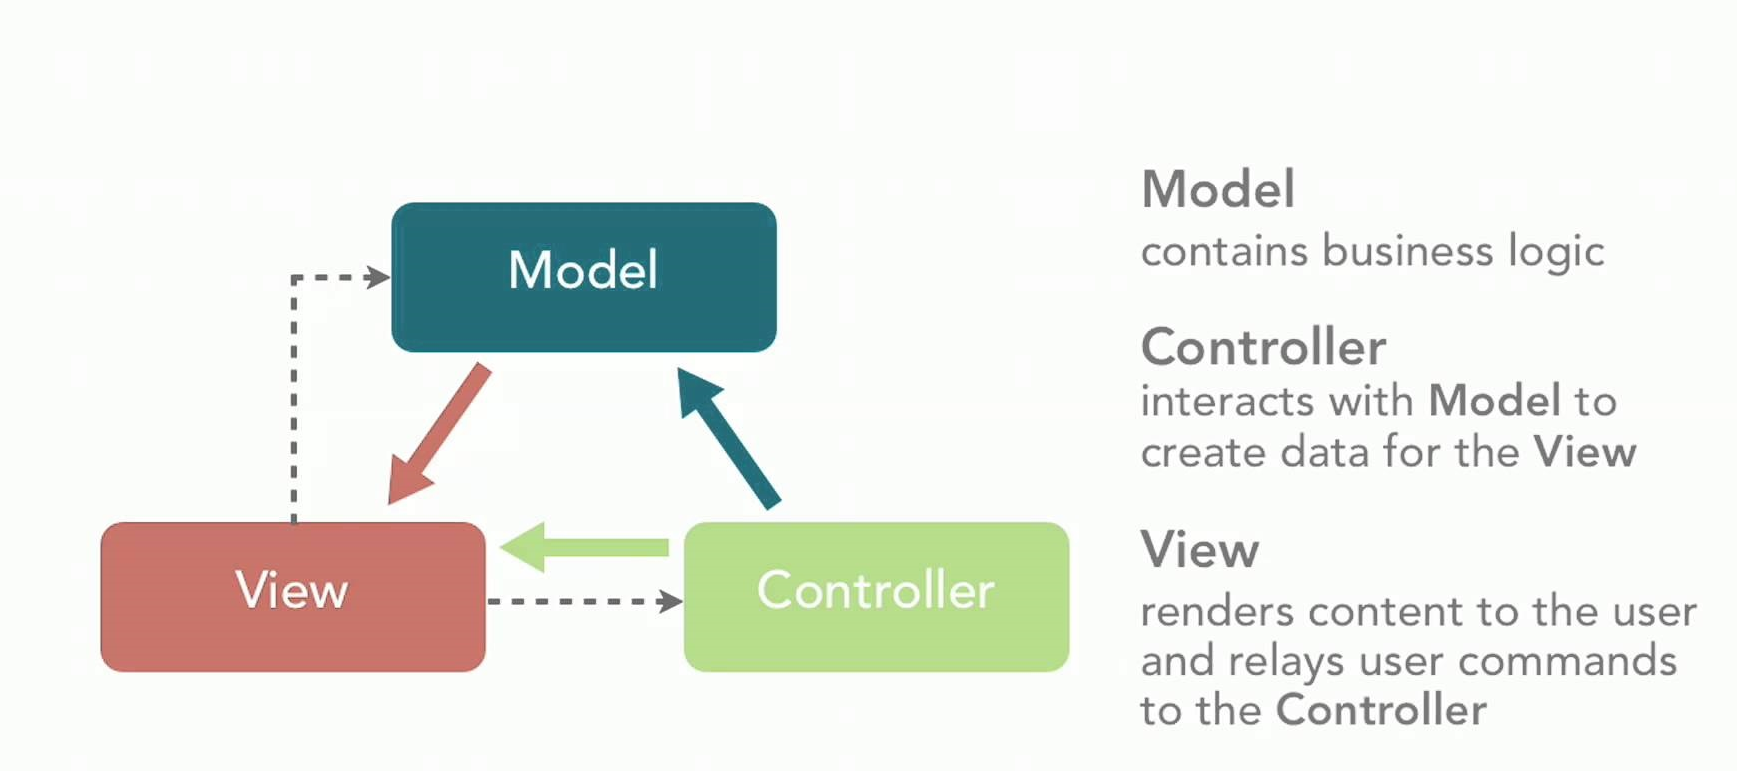
\includegraphics[width=\linewidth]{res/teoria/MVC.png}
    \caption{Struttura dell'MVC}
\end{figure}
\subsubsection{Layered Architecture}
Qui, ogni layer fornisce dei servizi a quello sopra. Il più basso contiene i core services. Si utilizza quando dobbiamo creare nuove parti sopra sistemi esistenti, e lo sviluppo è basato su vari team che lavorano a funzionalità diverse. Risolve anche i requirements di sicurezza multi-level. È un ottimo sostituto dei layer di implementazione, supporta la ridondanza, ma ha problemi di performance e rende difficile separare nettamente i layers.
\begin{figure}[H]
    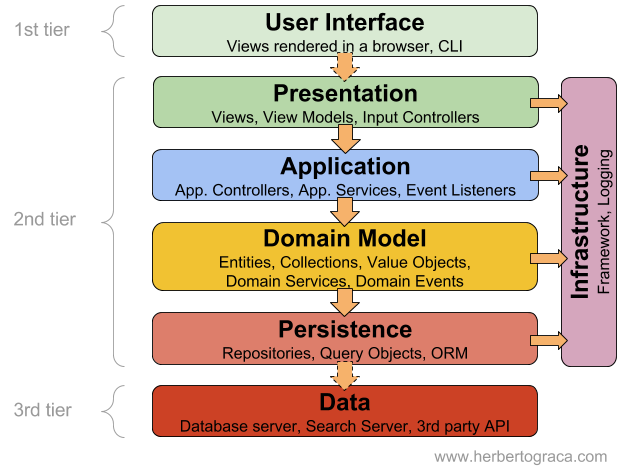
\includegraphics[width=\linewidth]{res/teoria/LayeredArchitecture.png}
\end{figure}
\subsubsection{Repository}
La repository è accessibile a tutti i componenti, che non interagiscono tra loro ma solo con la repository, che gestisce tutti i dati. Viene utilizzato quando abbiamo grandi volumi di informazioni e l'inclusione di dati nella repo triggera un'azione. Ha componenti indipendenti, propagazione dei cambiamenti, data management consistente, ma rischio di failure, comunicazione inefficiente e difficoltà di distribuzione della repo. 
\begin{figure}[H]
    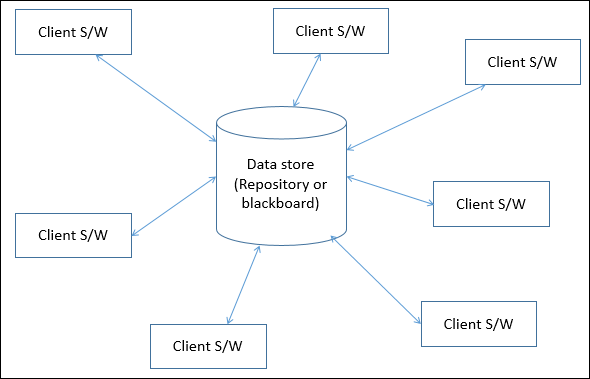
\includegraphics[width=\linewidth]{res/teoria/Repository.jpg}
\end{figure}
\subsubsection{Client-Server}
Utilizziamo client-server quando i dati devono essere accessibili da più posizioni, ed il carico è variabile (distribuzione dei server). Facilita la distribuzione di server e funzionalità, ma ogni server è un punto di failure, abbiamo performance imprevedibili, e problemi di gestione quando i server hanno diversi proprietari.
\paragraph{Thin e Fat client} Un thin client implementa l'interfaccia grafica, delegando al server ed alla rete le operazioni più pesanti. Un fat client, invece, esegue l'applicazione localmente, ed è quindi più complesso e potente. Gli aggiornamenti vanno installati su tutti i clients.
\paragraph{Three tier architecture}Qui, abbiamo due strati di server, ad esempio un web server che si connette ad un database server.
\subsubsection{Pipe and filter}
Il processo dei dati in un sistema è organizzato tramite una sequenza di componenti di processing, ognuno dei quali esegue una tipologia di trasformazione dei dati, i quali scorrono da un componente all'altro. Si utilizza in applicazioni di data processing nelle quali gli input sono processati in stadi separati per generare output. Un esempio sono i compilatori. Si prestano bene al riutilizzo ed ai business processes. Hanno evoluzione semplice e implementazione sequenziale/parallela. Devono però avere un formato di data transfer condiviso, e codificare/decodificare i dati. 
\subsection{Application architectures}
I sistemi di applicazioni possono essere raggruppati per il tipo di business. Siccome i business hanno molto in comune, i loro sistemi applicativi tendono ad avere un'architettura comune che riflette i requirements.
Un'architettura generica può essere configurata e adattata per creare un sistema che ha specifici requirements. Le application architectures sono un punto di partenza per il design, utilizzabili come checklist, come modalità organizzativa, come mezzo di riutilizzo, come vocabolario. 
\subsubsection{Centralized vs Decentralized}
Il design centralizzato rende facili le modifiche nella control structure, penalizzando però le performance del singolo control object. Quello decentralizzato divide le responsabilità, funziona bene con l'Object-Oriented e permette di dividere il carico. Per scegliere, osserviamo i sequence diagrams ed i control objects, verificandone la partecipazione. Se il sequence diagram assomiglia a una forchetta, centralizzato, se assomiglia a una sedia, decentralizzato. \textit{C'è scritto veramente?}
I sequence diagrams sono derivati dagli use case.
\begin{figure}[H]
    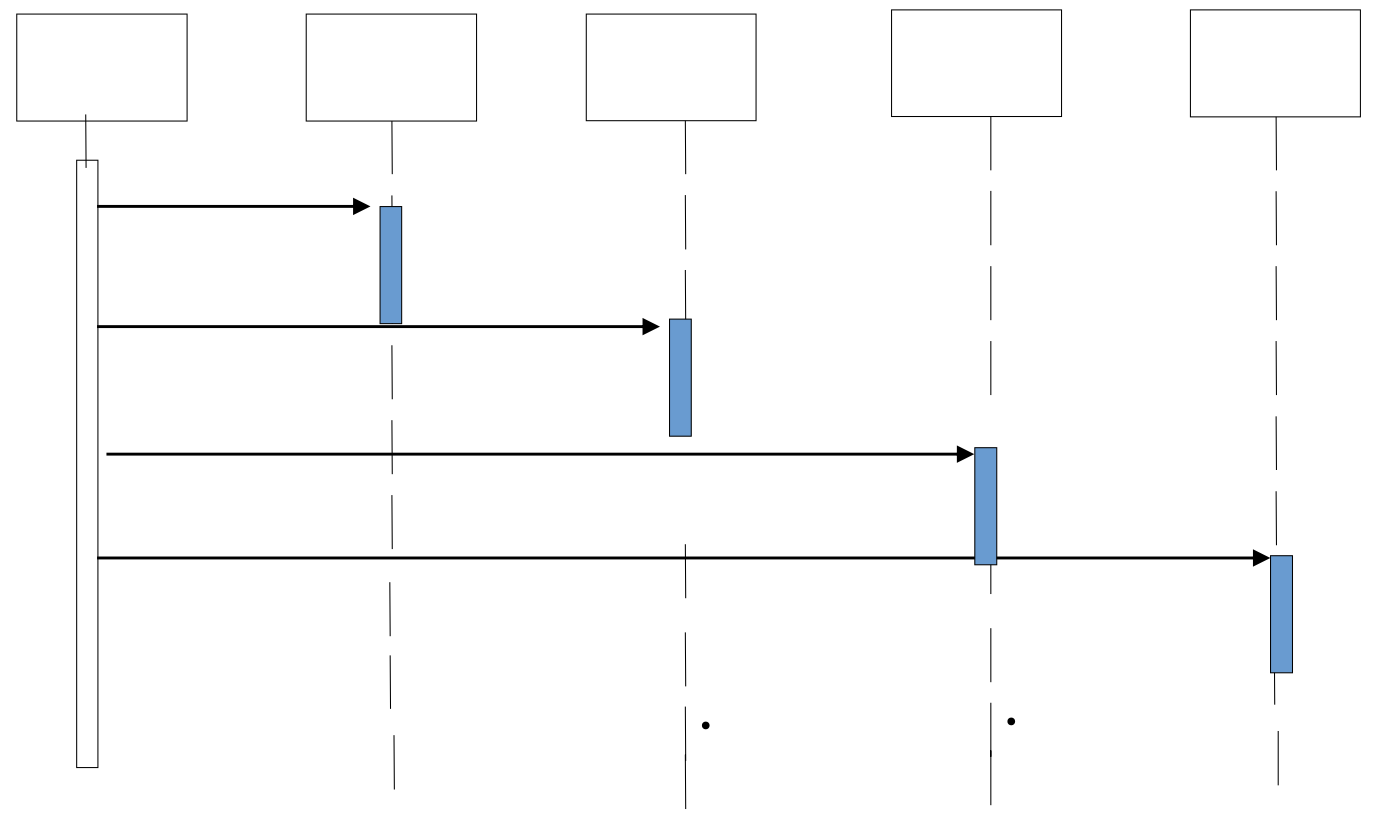
\includegraphics[width=0.5\linewidth]{res/teoria/Fork.png}
    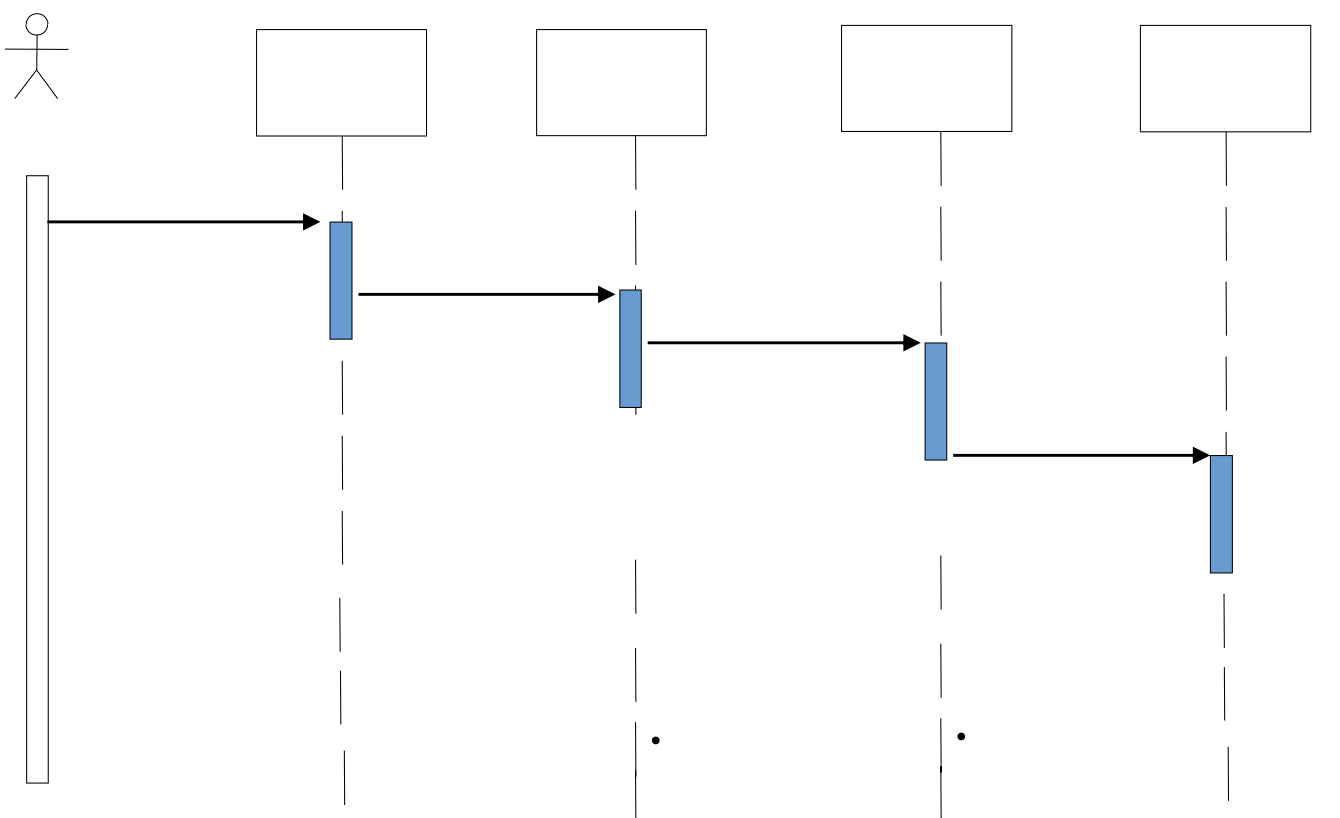
\includegraphics[width=0.5\linewidth]{res/teoria/Stair.png}
    \caption{Fork and Stair}
\end{figure}
Nella decentralizzata, le operazioni hanno forte connessione e sono eseguite sempre nello stesso ordine. Nella centralizzata, le operazioni possono cambiare ordine o quantità.
\subsubsection{Procedure vs Event Driven}
Nel procedure driven, il controllo è nel codice  del programma e l'utente ha poco controllo. Nell'event driven, il controllo risiede in un dispatcher che chiama funzioni via callbacks; l'utente ha qui molto controllo. 
\subsubsection{Vantaggi di una system architecture esplicita}
\begin{itemize}
    \item Comunicazione tra stakeholder: permette di discutere del sistema
    \item Analisi del sistema: permette di verificare i non functional requirements e fornire soluzioni
    \item Riutilizzo in larga scala: l'architettura è riutilizzabile su molti sistemi, la documentazione è di qualità, possiamo sviluppare product-line architectures 
    \item Definisce una struttura di divisione del lavoro e permette le stime
\end{itemize}
Il design dell'architettura è uno dei primi passi della metodologia agile, perché il refactor futuro è molto costoso.

\section{T18 - User Interface Design}
Gli utenti di un sistema spesso giudicano più l'interfaccia delle funzionalità: un'interfaccia realizzata male può causare errori o far disinstallare il software. Nel design, bisogna considerare i fattori umani: memoria a breve termine limitata, errori, capacità differenti, preferenze di interazione diverse. Dobbiamo quindi matchare le skills, esperienze ed aspettative degli utenti, considerandone però anche i limiti e le possibilità di errore. È utile basarsi su un set di design principles:
\begin{itemize}
    \item \textbf{User familiarity}: l'interfaccia dovrebbe essere basata su termini user-oriented e concetti, piuttosto che su concetti informatici.
    \item \textbf{Consistency}: il sistema dovrebbe avere un buon livello di consistenza, ad esempio comandi e menù nello stesso formato
    \item \textbf{Minimal surprise}: se un comando funziona in maniera conosciuta, l'utente dovrebbe poterne prevedere i risultati 
    \item \textbf{Recoverability}: il sistema dovrebbe fornire resilienza agli errori umani
    \item \textbf{User guidance}: bisognerebbe fornire sistemi di aiuto, manuali online\dots
    \item \textbf{User diversity}: bisognerebbe permettere una personalizzazione dell'interfaccia, ad esempio scegliendo la dimensione del font 
    \item \textbf{Real world mapping}: le informazioni dovrebbero essere presentate in un layout familiare
    \item \textbf{Consistency}: feature simili dovrebbero rimanere nello stesso posto e lavorare allo stesso modo 
    \item \textbf{Less is more}: le feature meno importanti non devono essere in mezzo ai coglioni
    \item \textbf{Anticipation}: nascondere feature inaccessibili
    \item \textbf{Customization}: fornire agli utenti esperti feature avanzate
    \item \textbf{Transparency}: l'interfaccia non dovrebbe coprire altri contenuti 
    \item \textbf{Contiguity}: inserire testi esplicativi vicino agli elementi grafici 
    \item \textbf{Memory load}: ricordare all'utente i dettagli 
    \item \textbf{User control}: identificare il responsabile delle azioni
    \item \textbf{Speak user's language}: istruzioni comprensibili, feedback, messaggi di errore 
\end{itemize}
Abbiamo diversi issues: come passare informazioni dall'utente al computer? Come passare informazioni dal computer all'utente? Sfruttiamo metafore per il design: un set di componenti visuali, azioni e procedure che ricordano conoscenze già acquisite dall'utente in altri domini. Alcuni tipi di componenti:
\begin{itemize}
    \item Windows: permettono di mostrare informazioni sullo schermo
    \item Icons: rappresentano diversi tipi di informazioni 
    \item Menus e pulsanti: selezionano comandi 
    \item Pointing: permette di selezionare in un menù 
    \item Graphics elements: mixabili con testo sulla stessa finestra 
\end{itemize}
Abbiamo più tipi di interazione: diretta, menu, form fill-in, comandi, linguaggio naturale. 
\paragraph{Direct manipulation} L'utente si sente in controllo del computer, ci mette poco ad imparare, ottiene feedback immediati. Però, la derivazione di un information space model è difficile, la navigazione può essere complessa e quindi richiedere molte risorse. 
\paragraph{Menu} I comandi sono presentati in una lista, lo sforzo di scrittura è minimale, gli errori improbabili. È possibile fornire aiuto contestuale. Però, le azioni complesse (and/or) sono difficili da rappresentare. I menù sono adatti a poche opzioni ed utenti non esperti, perché gli esperti preferiscono i comandi testuali. 
\paragraph{Form} Il form permette semplice data-entry, facilità di apprendimento, possibilità di verifica. Però richiede molto spazio a schermo e causa problemi quando l'utente non richiede esattamente ciò che è presente a schermo.
\paragraph{Command language} I comandi permettono uno sviluppo rapido, di complessità arbitraria ed interfacce minimali. Però, gli utenti dovranno ricordare il linguaggio: non è adatto ad utenti saltuari. Faranno inoltre errori, e sarà richiesta la possibilità di scrittura.
\paragraph{Linguaggio naturale} Esso è accessibile ad utenti inesperti ed estensibile facilmente. Però, il vocabolario è limitato e confinato a domini specifici. La tecnologia non è del tutto adatta a rendere queste interfacce accessibili ad utenti principianti (\textit{questa slide probabilmente è stata scritta nel 2004, quando Siri e Google Assistant non esistevano. Un aggiornamento non sarebbe male eh}), ma gli utenti esperti odiano dover scrivere molto. È necessario poter scrivere. 
\subsection{Design process}
Per il design è utile sviluppare un prototipo low-fidelity, che sia semplice ed economico anche nella modifica, in modo da far capire le caratteristiche principali senza concentrarsi sulle piccolezze estetiche. Bisogna spiegare le convenzioni agli utenti ed è difficile mostrare i comportamenti. Il processo di design consiste in:
\begin{enumerate}
    \item Analisi e comprensione delle attività dell'utente 
    \item Produzione di un prototipo su carta e valutazione con gli utenti 
    \item Design del prototipo dinamico e valutazione
    \item Design di un prototipo eseguibile, valutazione e implementazione finale 
\end{enumerate}
\subsubsection{Information presentation}
L'information presentation è costituita dallo studio di come presentare le informazioni all'utente, direttamente o trasformandole. L'MVC è una modalità che supporta più presentazioni di dati. 
Dobbiamo così porci più domande: 
\begin{itemize}
    \item L'utente è interessato alle informazioni o alle loro relazioni?
    \item Quando rapidamente variano?
    \item L'utente deve poter rispondere ai cambiamenti?
    \item È necessaria una manipolazione diretta?
    \item L'informazione è testuale o numerica? 
\end{itemize}
Distinguiamo tra presentazione digitale ed analogica: la prima è compatta e precisa, la seconda più instantanea alla vista. 
È utile sfruttare i colori come una dimensione aggiuntiva, ad esempio per evidenziare eventi eccezionali. Bisogna però stare attenti a non usarli troppo, limitandone il numero. Utilizziamo il cambiamento di colore per evidenziare cambiamenti nel sistema. Sfruttiamo i colori per supportare le attività dell'utente in maniera intelligente e consistente, stando attenti anche agli accostamenti. 
\paragraph{Messaggi di errore} Una corretta rappresentazione degli errori è fondamentale. I messaggi devono essere educati, coincisi, consistenti e costruttivi. Bisogna considerare anche altri fattori:
\begin{itemize}
    \item Contesto: il messaggio deve riflettere il contesto attuale
    \item Esperienza: un utente esperto ha bisogno di errori più concisi, un principiante di errori più \textit{verbose}
    \item Skill level: il messaggio deve riflettere le skill dell'utente
    \item Stile: i messaggi dovrebbero essere positivi 
    \item Culture: i messaggi dovrebbero essere familiari con la cultura del paese dove viene utilizzato il software
\end{itemize} 
\paragraph{Sistema di aiuto} Il sistema di aiuto non dev'essere un semplice manuale online: dobbiamo sfruttare le caratteristiche dinamiche dello schermo.
\subsection{Valutazione della user interface}
Dopo il lavoro di design, bisogna valutarlo vs. le specifiche di usability, seguendo parametri come \textit{learnability}, \textit{speed of operation}, \textit{robustness}, \textit{recoverability}, \textit{adaptability}. Utilizziamo più tecniche di valutazione:
\begin{itemize}
    \item Expert reviews 
    \item Questionari 
    \item Registrazioni video dell'utilizzo 
    \item Strumentazione di raccolta informazioni 
    \item Feedback online dagli utenti 
    \item Competitive usability testing
\end{itemize}
\section{T19 - UML Diagrams for system design}
\subsection{Component Diagram}
Il \textbf{component diagram} mostra gli elementi concettuali del business process (in UML1 erano componenti fisici), che forniscono o utilizzano interfacce per l'interazione con altri costrutti del sistema.
\paragraph{Component} Unità logica del sistema, ha interfacce definite ed è rappresentato da un rettangolo.
\paragraph{Interface} Descrive un gruppo di operazioni usate o create dai componenti. Un cerchio intero rappresenta un'interfaccia creata, mezzo ne rappresenta una required.
\paragraph{Dependencies} Le dipendenze sono indicate da frecce tratteggiate.
\paragraph{Ports} Le porte sono rappresentate da quadrati sul bordo. Sono usate per supportare l'esposizione di un'interfaccia required/created.
\subsubsection{Internal View}
Possiamo anche decidere di rappresentare l'interno di un componente come sottodiagramma

\subsection{Package Diagram}
Il \textbf{package diagram} rappresenta l'organizzazione degli elementi del modello in progetti di grandi dimensioni. I packages sono utilizzati per suddividere il sistema in entità logiche contenenti classi relazionate. Mostriamo i pacchetti come dei rettangoli con una sezione aggiunta in alto, e le dipendenze con frecce tratteggiate. Il nome viene inserito nella \textit{tab} in alto. Tramite le frecce, definiamo anche \textit{Merge}, \textit{Import}, \textit{Access}, \textit{Use}.

\subsection{Deployment Diagram}
Il \textbf{deployment diagram} mostra l'architettura di esecuzione del software, quindi processori, nodi, devices, le loro connessioni e la distribuzione dei file. Utilizziamo questi diagrammi per mostrare l'hardware e software di esecuzione. 
\paragraph{Node} Il nodo rappresenta l'entità principale, che esegue componenti. Può essere hardware o software.
\paragraph{Artifact} Gli artifacts sono elementi concreti che vengono causati dal processo di sviluppo. Possono essere librerie, configurazioni, archivi\dots
\paragraph{Communication Path} Mostra la connessione tra due nodi.
\paragraph{Manifest and deployment specification} Sono file che contengono configurazioni, ad esempio in XML.

\section{T20 - Object Oriented Design}
L'\textbf{Object Oriented Design} ha lo scopo di aggiungere dettagli alla requirements analysis e all'architecture model, prendendo decisioni riguardanti l'implementazione. Prepara l'implementazione attraverso decisioni sul design, ottimizza il system model, investiga alternative implementative. Gli obiettivi sono soprattutto non-functional. Esiste un gap tra il requirements gap ed il system gap, ed è proprio l'\textbf{object design gap}. Vogliamo costruire un Object Design Model che realizzi il modello Use Case, come base per l'implementazione. Vi sono però dei rischi di \textbf{incompletezza} e la presenza di attività \textbf{soggette ad errori.}
Gli obiettivi sono:
\begin{itemize}
    \item Riutilizzare le conoscenze del passato
    \item Riutilizzare funzionalità disponibili
    \item Supportare la definizione di robustezza e adattabilità
    \item Sviluppare nuove funzionalità
    \item Adattare un sistema esistente ad un nuovo ambiente/cliente
\end{itemize}
Notiamo \textbf{4 step fondamentali:}
\begin{enumerate}
    \item \textbf{Identificazione di soluzioni esistenti}: utilizzando l'ereditarietà, sfruttiamo componenti, soluzioni, design patterns.
    \item \textbf{Interface specification}: descriviamo precisamente ogni class interface.
    \item \textbf{Object Model Restructuring}: miglioriamo la comprensibilità ed estensibilità.
    \item \textbf{Object Model Optimization}: miglioriamo le performance
\end{enumerate}
\begin{figure}[H]
    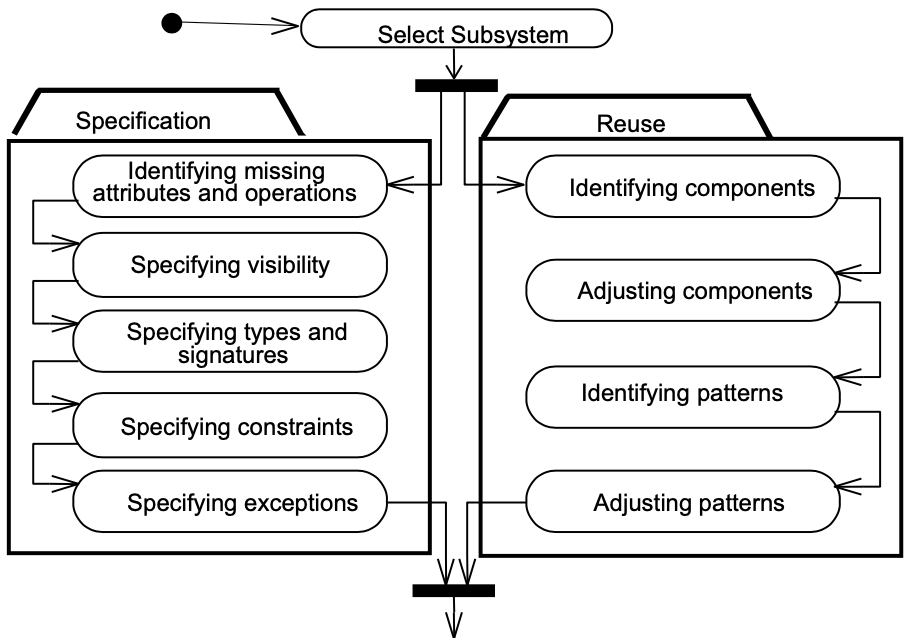
\includegraphics[width=0.5\linewidth]{res/teoria/OOD1.png}
    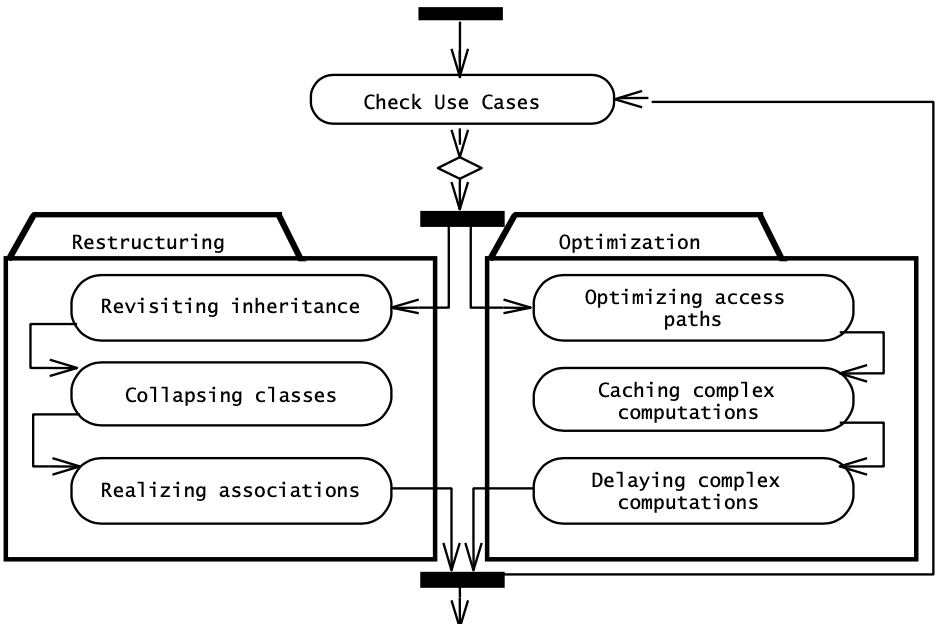
\includegraphics[width=0.5\linewidth]{res/teoria/OOD2.png}
\end{figure}
\subsection{Refactoring}
Il \textbf{refactoring} è un processo che cambia la struttura interna di un software senza cambiarne il comportamento. L'obiettivo è quello di rendere il software più facile da capire, più economico da modificare, e migliorarne l'aderenza ai requirements. Si può applicare sia ai design models che al codice. Viene spesso detto \textbf{remodeling}, quando applicato ai design models. Perché lo facciamo? \textbf{Migliora il design del software}, velocizzandolo, \textbf{rende il design più comprensibile}, \textbf{rende il debugging più facile}, \textbf{permette di programmare più velocemente}. Teniamo in conto tre principi:
\begin{itemize}
    \item Bisogna \textbf{evitare di aggiungere funzionalità durante il refactoring}
    \item Bisogna \textbf{verificare l'esistenza di test ottimali prima del refactoring}
    \item Procedere a \textbf{piccoli passi} localizzati
\end{itemize}
\subsection{Tecniche di riutilizzo}
\subsubsection{Ereditarietà}
Distinguiamo due utilizzi:
\begin{enumerate}
    \item Descrizione delle tassonomie: utilizzata durante la requirements analysis, identifica oggetti del dominio che hanno una relazione, allo scopo di rendere l'analysis model più comprensibile. 
    \item Specifica delle interfacce: usata durante l'object design, identifica le signatures degli oggetti identificati, allo scopo di aumentare il riutilizzo, la modificabilità, l'estensione.
\end{enumerate}
Distinguiamo, inoltre, tra \textbf{inheritance} (white-box reuse), e \textbf{composition} (black-box reuse). Nella prima i prodotti dello sviluppo (modelli, system/object design, codice) devono essere disponibili, e sfruttiamo implementation e specification. La seconda necessita solo di alcuni prodotti, al minimo gli eseguibili, e crea gli oggetti come aggregazione di quelli esistenti. Abbiamo più ragioni per le quali può essere necessaria la creazione di oggetti:
\begin{itemize}
    \item I boundary objects necessitano di componenti della GUI 
    \item Gli entity objects necessitano di componenti di data management specifici 
    \item L'implementazione di algoritmi potrebbe necessitare di oggetti per salvare valori 
    \item Le operazioni di alto livello potrebbero essere decomposte in operazioni di basso livello 
    \item Gli use case actors dovrebbero essere definiti da interfacce 
    \item Alcune classi di data collection potrebbero essere definite per salvare dati sugli attori 
    \item Almeno una classe di avvio deve esistere per far partire il software
    \item Potrebbero essere necessarie classi controller e coordinator per regolare l'esecuzione 
\end{itemize}
Vi è anche la possibilità di unire oggetti, per scelte di design: implementare un'entità come attributo, o come classe separata con associazioni ad altre classi. Le associazioni sono più flessibili degli attributi, ma spesso introducono indirection (mancanza di chiarezza) non necessaria. Troviamo ereditarietà per generalizzazione (ossia partendo dalle subclasses) o per specializzazione (partendo dalle superclasses). Per aumentare l'ereditarietà, riarrangiamo le classi per prepararle, cerchiamo di trasformare le superclasses in interfacce astratte (bridge pattern), verifichiamo se è possibile mappare le classi di un subsystem in una gerarchia di ereditarietà. Possiamo trovare dei problemi durante questo processo: non dobbiamo infatti esagerare implementando interfacce con metodi inutilizzati.
\subsubsection{Delegation}
La \textbf{delegation} è un modo di rendere la composizione potente quanto l'ereditarietà. Nella delegation, due oggetti sono coinvolti nella gestione di una richiesta del client: il \textbf{receiver} delega le operazioni al \textbf{delegate}, assicurandosi che il client non utilizzi il delegate in modo errato. I due metodi diversi hanno pro e contro: la delegation è più flessibile ma inefficiente, l'inheritance è facile da usare, supportata da più linguaggi, ma espone una subclass ai dettagli della classe parent, ed ogni modifica nel parent costringe le subclasses a cambiare.
\paragraph{Contraction}
Il goal della contraction è rendere le operazioni della superclass invisibili, implementando metodi nella superclasse ed overridandoli con metodi vuoti nella subclass. Questo processo andrebbe evitato, perché la superclass contiene operazioni che non hanno senso nella subclass, non \textit{fitta} nella tassonomia della superclasse, e viola il principio di sostituzione di Liskov. 
\paragraph{Raffinare le associazioni con l'aggregazione}
Aggiungiamo molteplicità e ruoli, decidendo \textit{whole} e \textit{part}, poi guardiamo alla molteplicità del whole: se è 1, usiamo la composizione, altrimenti aggregazione. Aggiungiamo infine la navigabilità dal whole alla part.
\paragraph{Raffinare le associazioni con la reification} 
La \textbf{reification} riguarda il trattamento di una cosa astratta come se fosse concreta; nei termini object-oriented, intendiamo la caratterizzazione di qualcosa nei termini di \textbf{oggetto}. Nel contesto del design, il concetto è applicato alle relazioni tra oggetti o stati di un oggetto. 
\subsection{Packaging design}
Il \textbf{packaging design} impacchetta il design in unità discrete che possono essere modificate, compilate, collegate, riutilizzate. Costruiscono moduli fisici, idealmente un pacchetto per subsystem. La system decomposition potrebbe non essere buona per l'implementazione. Due principi base: minimizzare il coupling, massimizzare la cohesion. Come fare?
\begin{enumerate}
    \item Partire con un'interfaccia per ogni subsystem 
    \item Limitare il numero di operazioni dell'interfaccia ($7 \mp 2$)
    \item Se l'interfaccia ha troppe operazioni, riconsideriamo il numero di interfacce 
    \item Se abbiamo troppe poche interfacce, riconsideriamo il numero di subsystems
\end{enumerate}
Per definire le classi, aggiungiamo prima gli attributi, poi i metodi, e li inseriamo nell'object model. Infine aggiungiamo gli invariants. Per i metodi, invece, decidiamo le pre-conditions, le post-conditions, e lavoriamo su pseudocode, flowcharts, UML per specificare l'algoritmo.
\subsection{Information hiding}
Per ottenere un buon \textbf{information hiding}, definiamo interfacce pubbliche, applicando il "need to know" principle: meno dettagli una classe deve sapere, più facile è cambiarla/non rovinarla con cambiamenti. Il tradeoff qui è information hiding vs efficiency. Elenchiamo alcuni principi:
\begin{itemize}
    \item Solo le operazioni di una classe ne possono manipolare gli attributi 
    \item Nascondere gli oggetti esterni al subsystem boundary: definire le interfacce astratte che mediano tra il mondo esterno ed il sistema
    \item Non applicare ad un'operazione i risultati di un'altra operazione
\end{itemize}
\section{T22 - Testing}
Distinguiamo in 4 componenti:
\begin{itemize}
    \item Test plan
    \item Test specification 
    \item Test oracle
    \item Test cases
\end{itemize}
\subsection{Componenti del testing}
\subsubsection{Test Plan}
Il \textbf{test plan} è utilizzato per dimostrare che il software è privo di falle e si comporta come richiesto dai requirements. Decompone il processo in test specifici, utilizzando specifici data items e valori. 
\subsubsection{Test Specification}
Documenta lo scopo di un test; in caso di test compositi, documenta la relazione tra le parti ed il whole test. Descrive le condizioni che indicano quando il test è completo. In generale, è un modo per valutare i risultati. 
\subsubsection{Test Oracle}
È un set di risultati predetti per un set di test, e si usa per determinare il successo del testing. È estremamente difficile da creare, attraverso la requirements specification. 
\subsubsection{Test Cases}
È un set di input al sistema. Un testing di successo è basato sulla scelta dei giusti test cases.

\subsection{Test suite}
Ovviamente bisogna testare il codice per farlo funzionare la prima volta, facendo \textit{ad hoc testing} o costruendo una test suite. La seconda riduce il numero totale di bug, rende il codice più mantenibile e refactorabile, ma richiede più programmazione e tempo. Distinguiamo tra due tecniche di testing: \textbf{glass box testing}, in cui esaminiamo il codice, e \textbf{black box testing}, basato sulla conoscenza del risultato atteso. 
\subsection{Tipologie di testing}
\begin{figure}[H]
    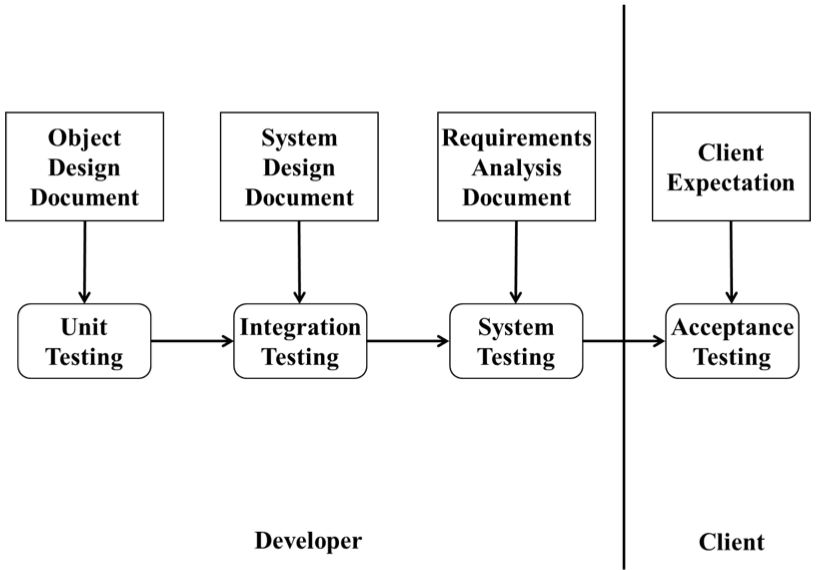
\includegraphics[width=0.7\linewidth]{res/teoria/TestingTypes.png}
\end{figure}
\subsubsection{Unit testing}
Lo \textbf{unit testing} testa le singole unità che compongono il sistema, allo scopo di trovare falle in algoritmi, dati, sintassi. Definiamo un set di test cases e ne valutiamo i risultati. Questo test è fatto dagli sviluppatori per assicurarsi che l'unità sia codificata correttamente e funzioni come ci si aspetta.
Distinguiamo, anzitutto, tra \textbf{static testing}(analisi, code review) e \textbf{dynamic testing} (black-box, white-box).
\paragraph{Black-box testing} Questo tipo di testing si concentra sul comportamento I/O, e richiede un test oracle. L'obiettivo è ridurre il numero di test cases  tramite equivalence partitioning. Dividiamo input validi ed invalidi in classi di equivalenza, scegliamo i test cases per ogni classe di equivalenza. Per scegliere i test case, notiamo che l'input è valido in un range di valori, e scegliamo i test case da quelli sotto il range, nel range, oltre il range. L'input è valido solo se facente parte di un set discreto: prendiamo un test case valido, uno invalido. 
\paragraph{White-box testing} Non è possibile testare tutti i percorsi, cerchiamo di assicurarci che ogni linea di codice sia testata. Il glass-box testing ha dei limiti: un pezzo di codice definisce più execution paths, ed un buon test case deve provarli tutti, arrivando a quantità di test case enormi. 
\paragraph{Euristiche} Per ottenere gli unit tests:
\begin{enumerate}
    \item Definiamo gli unit tests
    \item Creiamo i test cases 
    \item Eliminiamo duplicati tra i test cases 
    \item Controlliamo staticamente il codice 
    \item Creiamo un test harness, i.e. una collezione di test cases 
    \item Descriviamo il test oracle 
    \item Eseguiamo i test cases 
    \item Compariamo i risultati con il test oracle
\end{enumerate}
Per la selezione dei test cases, utilizziamo la conoscenza dei functional requirements, il design knowledge del sistema, delle data structures, degli algoritmi. Utilizziamo anche la conoscenza dell'implementazione di algoritmi e strutture dati. 
\subsubsection{Integration testing}
L'integration testing testa un gruppo di subsystems, ed eventualmente l'intero sistema. È fatto dagli sviluppatori per testare le interfacce tra subsystems. L'intero sistema è visto come una collezione di subsystems, determinati durante il system e object design. L'obiettivo è testare tutte le interfacce tra subsystems e la loro interazione, strategizzando l'ordine con cui i subsystems sono testati. Perché lo facciamo? Gli unit tests funzionano solo in isolazione, ma spesso le falle sono nell'interazione. Spesso molti componenti riutilizzati non possono essere unit tested. Le falle non trovate durante l'integration testing verranno scovate in produzione, il che non va mai bene.
Definiamo alcune componenti:
\paragraph{Driver} È un componente che chiama l'unità testata e controlla i test cases 
\paragraph{Stub/Double} è un componente che simula la presenza di un altro, rispondendo alle chiamate con dati falsi. Non deve comportarsi esattamente come chi sostituisce, ma deve fornire circa la stessa API. Ne distinguiamo 4 tipi: 
\begin{itemize}
    \item \textbf{Dummy}: è utilizzato come segnaposto, passato come parametro ma mai utilizzato 
    \item \textbf{Stub}: è un oggetto che forza il sistema verso il path che vogliamo testare
    \item \textbf{Mock}: ritorna valori hardcoded o precaricati 
    \item \textbf{Fake}: rimpiazza l'originale con un'implementazione alternativa 
\end{itemize}
\paragraph{Integration testing strategies}
Distinguiamo inoltre varie strategie di integration testing:
\begin{itemize}
    \item \textbf{Big Bang Integration}: porta difficoltà nella fault isolation, ma non necessita di drivers o stubs, è una pratica comune dell'agile
    \item \textbf{Bottom-Up Integration}: testa i sistemi più importanti per ultimi, necessita di driver ma non stubs, è utile per i sistemi object-oriented e real time 
    \item \textbf{Top-Down Integration}: i test cases possono essere definiti sulla base di funzionalità di sistema, non c'è bisogno di drivers ma gli stub sono difficoltosi e in grande quantità. In secundis, le utilità di basso livello sono testate tardi.
    \item \textbf{Sandwich Testing}: top e bottom sono fatti insieme, senza testare i subsystem singoli e le loro interfacce prima dell'integrazione. È meno sistematico degli altri due e rende più complicata la failure isolation
    \item \textbf{Modified Sandwich}: Testa in parallelo il middle layer con driver e stubs, il top layer con stubs, il bottom layer con drivers. Testa in parallelo il top layer che accede al middle, ed il middle che accede al bottom. 
\end{itemize}

\subsubsection{System Testing}
Il system testing testa l'intero sistema, ed è fatto dagli sviluppatori allo scopo di determinare se il sistema rispetta i requirements funzionali e di performance. I test cases sono creati partendo dal requirements analysis document o dallo user manual. I test cases sono centrati attorno ai requirements e alle funzioni chiave, ed il sistema è trattato come una black box. Gli unit test cases sono riutilizzati, ed i nuovi test cases vanno sviluppati. 
\paragraph{Performance testing} Il goal è tentare di violare i non-functional requirements, testando come il sistema si comporta quando è sovraccaricato, o in ordini non usuali di esecuzione, o con grandi volumi di dati. Citiamo, ad esempio: stress testing, security testing, volume testing, configuration testing, quality testing, recovery testing\dots
\paragraph{Acceptance Testing} Il goal è dimostrare che il sistema è pronto per l'utilizzo, con test e svolti scelti dal cliente. Distinguiamo tra \textbf{alpha test}, in cui si testa nell'ambiente di sviluppo, e \textbf{beta test}, in cui si testa nell'ambiente del cliente.
\subsection{Object-Oriented testing}
I componenti testati sono classi, istanziate come oggetti. Meno granulare di test su funzioni individuali, quindi gli approcci al white-box testing vanno estesi. Non c'è inoltre un "top" ovvio per il top-down. Distinguiamo 4 livelli: test delle operazioni associate alle classi, test delle classi, test di cluster di oggetti cooperanti, test del sistema completo. 
\paragraph{Object Class Testing} Un test completo di una classe testa tutte le operazioni associate, gli attributi, tutti gli stati. L'ereditarietà rende questo test più complesso.
\paragraph{Object Integration}
I livelli di integrazione sono meno distinti nei sistemi object-oriented. Il cluster testing si occupa di integrare e testare cluster di oggetti, identificati tramite la conoscenza delle operazioni e le feature implementate nel cluster. Distinguiamo tre approcci: \textbf{use-case or scenario testing}, basato sulle interazioni utente, \textbf{thread testing}, basato sulle risposte del sistema, \textbf{object interaction testing}, testante le interazioni che si fermano quando un'istanza non chiama servizi di un altro oggetto. 
\paragraph{Ereditarietà, polimorfismo, dynamic binding}
\begin{itemize}
    \item Ereditarietà: i metodi ereditati devono essere ritestati nelle subclasses: il contesto delle superclasses potrebbe essere incompleto 
    \item Polimorfismo: i parametri devono avere più di un set di valori e un'operazione deve essere implementata da più di un metodo 
    \item Dynamic binding: i metodi che implementano un'operazione sono sconosciuti fino al runtime 
\end{itemize}
\paragraph{Continuous testing}
Il continuous testing consiste in build e relativo testing ogni giorno, in modo che il sistema sia sempre eseguibile. Richiede dei tool di supporto, come un continuous build server, test automatizzati, tool supported refactoring, issue tracking\dots
\printglossary
\end{document}